% Options for packages loaded elsewhere
\PassOptionsToPackage{unicode}{hyperref}
\PassOptionsToPackage{hyphens}{url}
%
\documentclass[
]{article}
\usepackage{amsmath,amssymb}
\usepackage{iftex}
\ifPDFTeX
  \usepackage[T1]{fontenc}
  \usepackage[utf8]{inputenc}
  \usepackage{textcomp} % provide euro and other symbols
\else % if luatex or xetex
  \usepackage{unicode-math} % this also loads fontspec
  \defaultfontfeatures{Scale=MatchLowercase}
  \defaultfontfeatures[\rmfamily]{Ligatures=TeX,Scale=1}
\fi
\usepackage{lmodern}
\ifPDFTeX\else
  % xetex/luatex font selection
\fi
% Use upquote if available, for straight quotes in verbatim environments
\IfFileExists{upquote.sty}{\usepackage{upquote}}{}
\IfFileExists{microtype.sty}{% use microtype if available
  \usepackage[]{microtype}
  \UseMicrotypeSet[protrusion]{basicmath} % disable protrusion for tt fonts
}{}
\makeatletter
\@ifundefined{KOMAClassName}{% if non-KOMA class
  \IfFileExists{parskip.sty}{%
    \usepackage{parskip}
  }{% else
    \setlength{\parindent}{0pt}
    \setlength{\parskip}{6pt plus 2pt minus 1pt}}
}{% if KOMA class
  \KOMAoptions{parskip=half}}
\makeatother
\usepackage{xcolor}
\usepackage[margin=1in]{geometry}
\usepackage{graphicx}
\makeatletter
\newsavebox\pandoc@box
\newcommand*\pandocbounded[1]{% scales image to fit in text height/width
  \sbox\pandoc@box{#1}%
  \Gscale@div\@tempa{\textheight}{\dimexpr\ht\pandoc@box+\dp\pandoc@box\relax}%
  \Gscale@div\@tempb{\linewidth}{\wd\pandoc@box}%
  \ifdim\@tempb\p@<\@tempa\p@\let\@tempa\@tempb\fi% select the smaller of both
  \ifdim\@tempa\p@<\p@\scalebox{\@tempa}{\usebox\pandoc@box}%
  \else\usebox{\pandoc@box}%
  \fi%
}
% Set default figure placement to htbp
\def\fps@figure{htbp}
\makeatother
\setlength{\emergencystretch}{3em} % prevent overfull lines
\providecommand{\tightlist}{%
  \setlength{\itemsep}{0pt}\setlength{\parskip}{0pt}}
\setcounter{secnumdepth}{-\maxdimen} % remove section numbering
\usepackage{bookmark}
\IfFileExists{xurl.sty}{\usepackage{xurl}}{} % add URL line breaks if available
\urlstyle{same}
\hypersetup{
  pdftitle={Dissecting lentil crop growth in contrasting environments using digital imaging and and genome-wide association studies},
  pdfauthor={Derek Michael Wright derek.wright@usask.ca},
  hidelinks,
  pdfcreator={LaTeX via pandoc}}

\title{Dissecting lentil crop growth in contrasting environments using
digital imaging and and genome-wide association studies}
\usepackage{etoolbox}
\makeatletter
\providecommand{\subtitle}[1]{% add subtitle to \maketitle
  \apptocmd{\@title}{\par {\large #1 \par}}{}{}
}
\makeatother
\subtitle{\emph{The Plant Phenome Journal}. (\textbf{2025}) 8(1):
e70040.}
\author{Derek Michael Wright
\href{mailto:derek.wright@usask.ca}{\nolinkurl{derek.wright@usask.ca}}}
\date{01-08-2025}

\begin{document}
\maketitle

{
\setcounter{tocdepth}{2}
\tableofcontents
}
\begin{center}\rule{0.5\linewidth}{0.5pt}\end{center}

\begin{quote}
\href{https://doi.org/10.1002/ppj2.70040}{Derek Wright, Sandesh Neupane,
Karsten Neilson, Tania Gioia \& Kirstin E Bett. \textbf{Dissecting
lentil crop growth in contrasting environments using digital imaging and
and genome-wide association studies}. \emph{The Plant Phenome Journal}.
(\textbf{2025}) 8(1): e70040. doi.org/10.1002/ppj2.70040}
\end{quote}

which is follow-up to:

\begin{quote}
\begin{itemize}
\tightlist
\item
  \href{https://doi.org/10.1002/tpg2.20269}{Sandesh Neupane, Derek
  Wright, Raul Martinez, Jakob Butler, Jim Weller, Kirstin
  Bett.\textbf{Focusing the GWAS \emph{Lens} on days to flower using
  latent variable phenotypes derived from global multi-environment
  trials}. \emph{The Plant Genome}. (\textbf{2022}) 16(1): e20269.
  doi.org/10.1002/tpg2.20269}
\item
  \url{https://github.com/derekmichaelwright/AGILE_LDP_GWAS_Phenology}
\end{itemize}
\end{quote}

\begin{quote}
\begin{itemize}
\tightlist
\item
  \href{https://doi.org/10.1002/ppp3.10158}{Derek M Wright, Sandesh
  Neupane, Taryn Heidecker, Teketel A Haile, Clarice J Coyne, Rebecca J
  McGee, Sripada Udupa, Fatima Henkrar, Eleonora Barilli, Diego
  Rubiales, Tania Gioia, Giuseppina Logozzo, Stefania Marzario, Reena
  Mehra, Ashutosh Sarker, Rajeev Dhakal, Babul Anwar, Debashish Sarker,
  Albert Vandenberg, and Kirstin E. Bett. \textbf{Understanding
  photothermal interactions can help expand production range and
  increase genetic diversity of lentil (\emph{Lens culinaris} Medik.)}.
  \emph{Plants, People, Planet}. (\textbf{2021}) 3(2): 171-181.}
\item
  \url{https://github.com/derekmichaelwright/AGILE_LDP_Phenology}
\end{itemize}
\end{quote}

\begin{center}\rule{0.5\linewidth}{0.5pt}\end{center}

Contents

\begin{quote}
\begin{itemize}
\tightlist
\item
  \url{https://github.com/derekmichaelwright/AGILE_LDP_GWAS_Phenology}
\item
  \href{https://github.com/derekmichaelwright/AGILE_LDP_UAV/raw/master/README.pdf}{View
  as pdf}
\item
  \href{https://derekmichaelwright.github.io/AGILE_LDP_UAV/README.html}{View
  as HTML}
\item
  \href{https://derekmichaelwright.github.io/AGILE_LDP_UAV/Growth_Rates_Vignette.html}{Source
  Code Vignette (Growth\_Rates\_Vignette.html)}
\end{itemize}
\end{quote}

\begin{itemize}
\tightlist
\item
  \hyperref[raw-data-ux26-growth-curve-modeling]{Raw Data \& Growth
  Curve Modeling}
\item
  \hyperref[figures]{Figures}
\item
  \hyperref[supplemental-tables]{Supplemental Tables}
\item
  \hyperref[supplemental-figures]{Supplemental Figures}
\item
  \hyperref[additional-figures]{Additional Figures}
\end{itemize}


\includegraphics[width=0.5\linewidth,height=\textheight,keepaspectratio]{Additional/img_Agile.png}


\includegraphics[width=0.5\linewidth,height=\textheight,keepaspectratio]{Additional/img_P2IRC.png}

\subsection{Collaborators}\label{collaborators}

\begin{itemize}
\tightlist
\item
  Department of Plant Sciences and Crop Development Centre, University
  of Saskatchewan, Saskatoon, Saskatchewan, Canada
\item
  School of Agriculture, Forestry, Food and Environmental Sciences,
  University of Basilicata, Potenza, Italy
\end{itemize}

\begin{center}\rule{0.5\linewidth}{0.5pt}\end{center}

\section{Raw Data \& Growth Curve
Modeling}\label{raw-data-growth-curve-modeling}

\begin{quote}
\begin{itemize}
\tightlist
\item
  \href{https://github.com/derekmichaelwright/AGILE_LDP_UAV/Additional/ggDroneCheck_It17.pdf}{Additional/ggDroneCheck\_It17.pdf}
\item
  \href{https://github.com/derekmichaelwright/AGILE_LDP_UAV/Additional/ggDroneCheck_Ro17.pdf}{Additional/ggDroneCheck\_Ro17.pdf}
\item
  \href{https://github.com/derekmichaelwright/AGILE_LDP_UAV/Additional/ggDroneCheck_Su17.pdf}{Additional/ggDroneCheck\_Su17.pdf}
\item
  \href{https://github.com/derekmichaelwright/AGILE_LDP_UAV/Additional/ggDroneCheck_Su18.pdf}{Additional/ggDroneCheck\_Su18.pdf}
\end{itemize}
\end{quote}

\begin{center}\rule{0.5\linewidth}{0.5pt}\end{center}

\subsection{Metaponto, Italy 2017}\label{metaponto-italy-2017}

\begin{quote}
\begin{itemize}
\tightlist
\item
  \href{https://derekmichaelwright.github.io/AGILE_LDP_UAV/Additional/ggpGrowthCurves_It17_volume.html}{Additional/ggpGrowthCurves\_It17\_volume.html}
\end{itemize}
\end{quote}

\pandocbounded{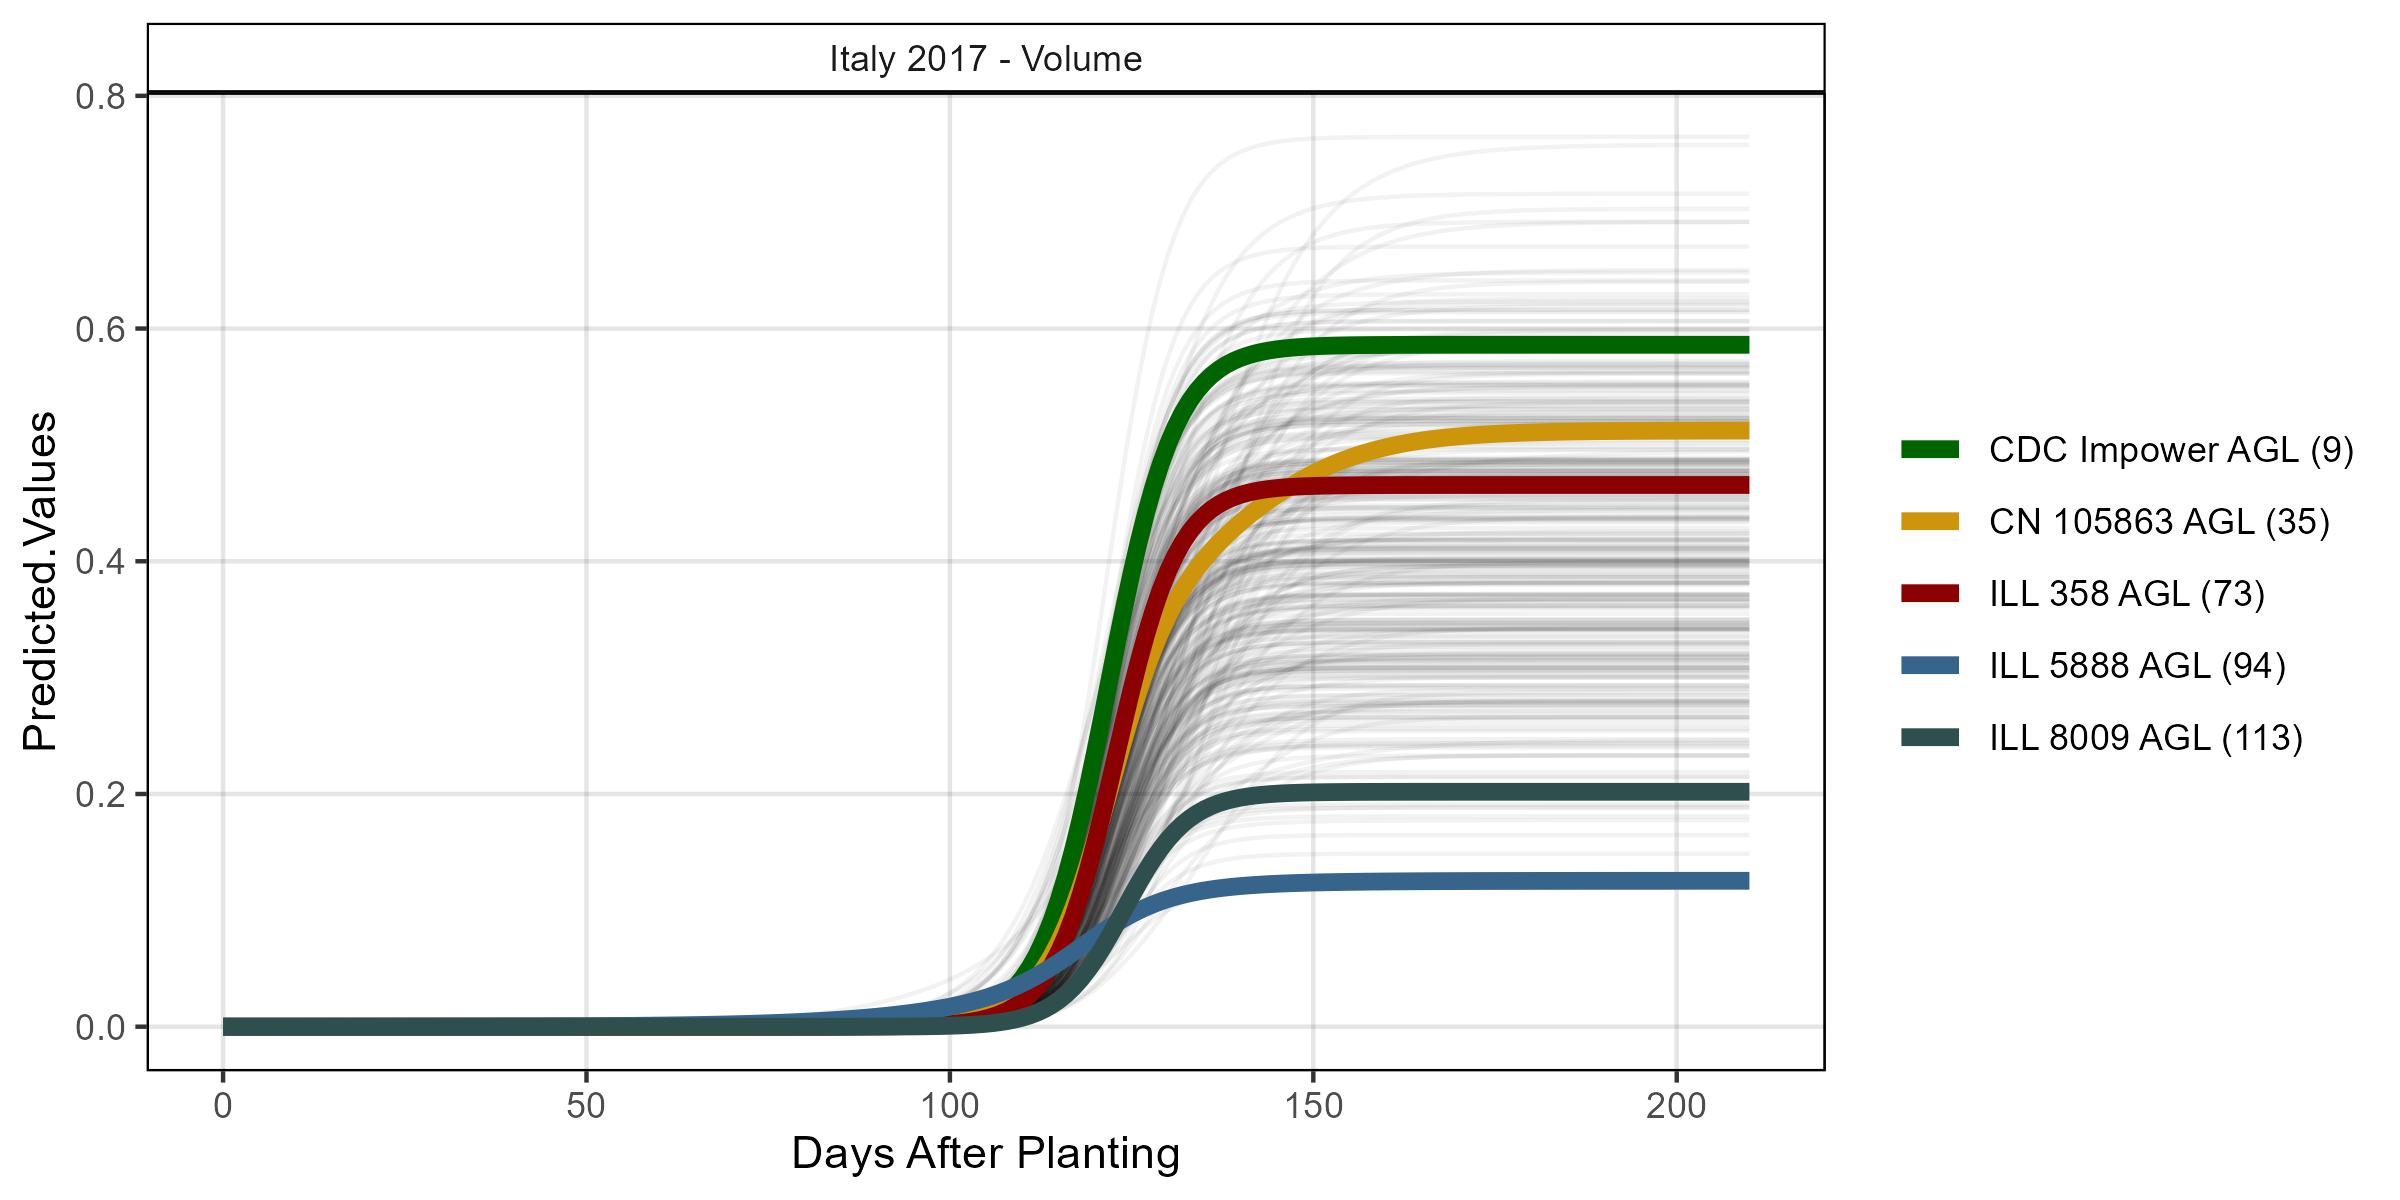
\includegraphics[keepaspectratio]{Additional/ggGrowthCurves_It17_volume.png}}

\begin{quote}
\begin{itemize}
\tightlist
\item
  \href{https://derekmichaelwright.github.io/AGILE_LDP_UAV/Additional/ggpGrowthCurves_It17_area.html}{Additional/ggpGrowthCurves\_It17\_area.html}
\end{itemize}
\end{quote}

\pandocbounded{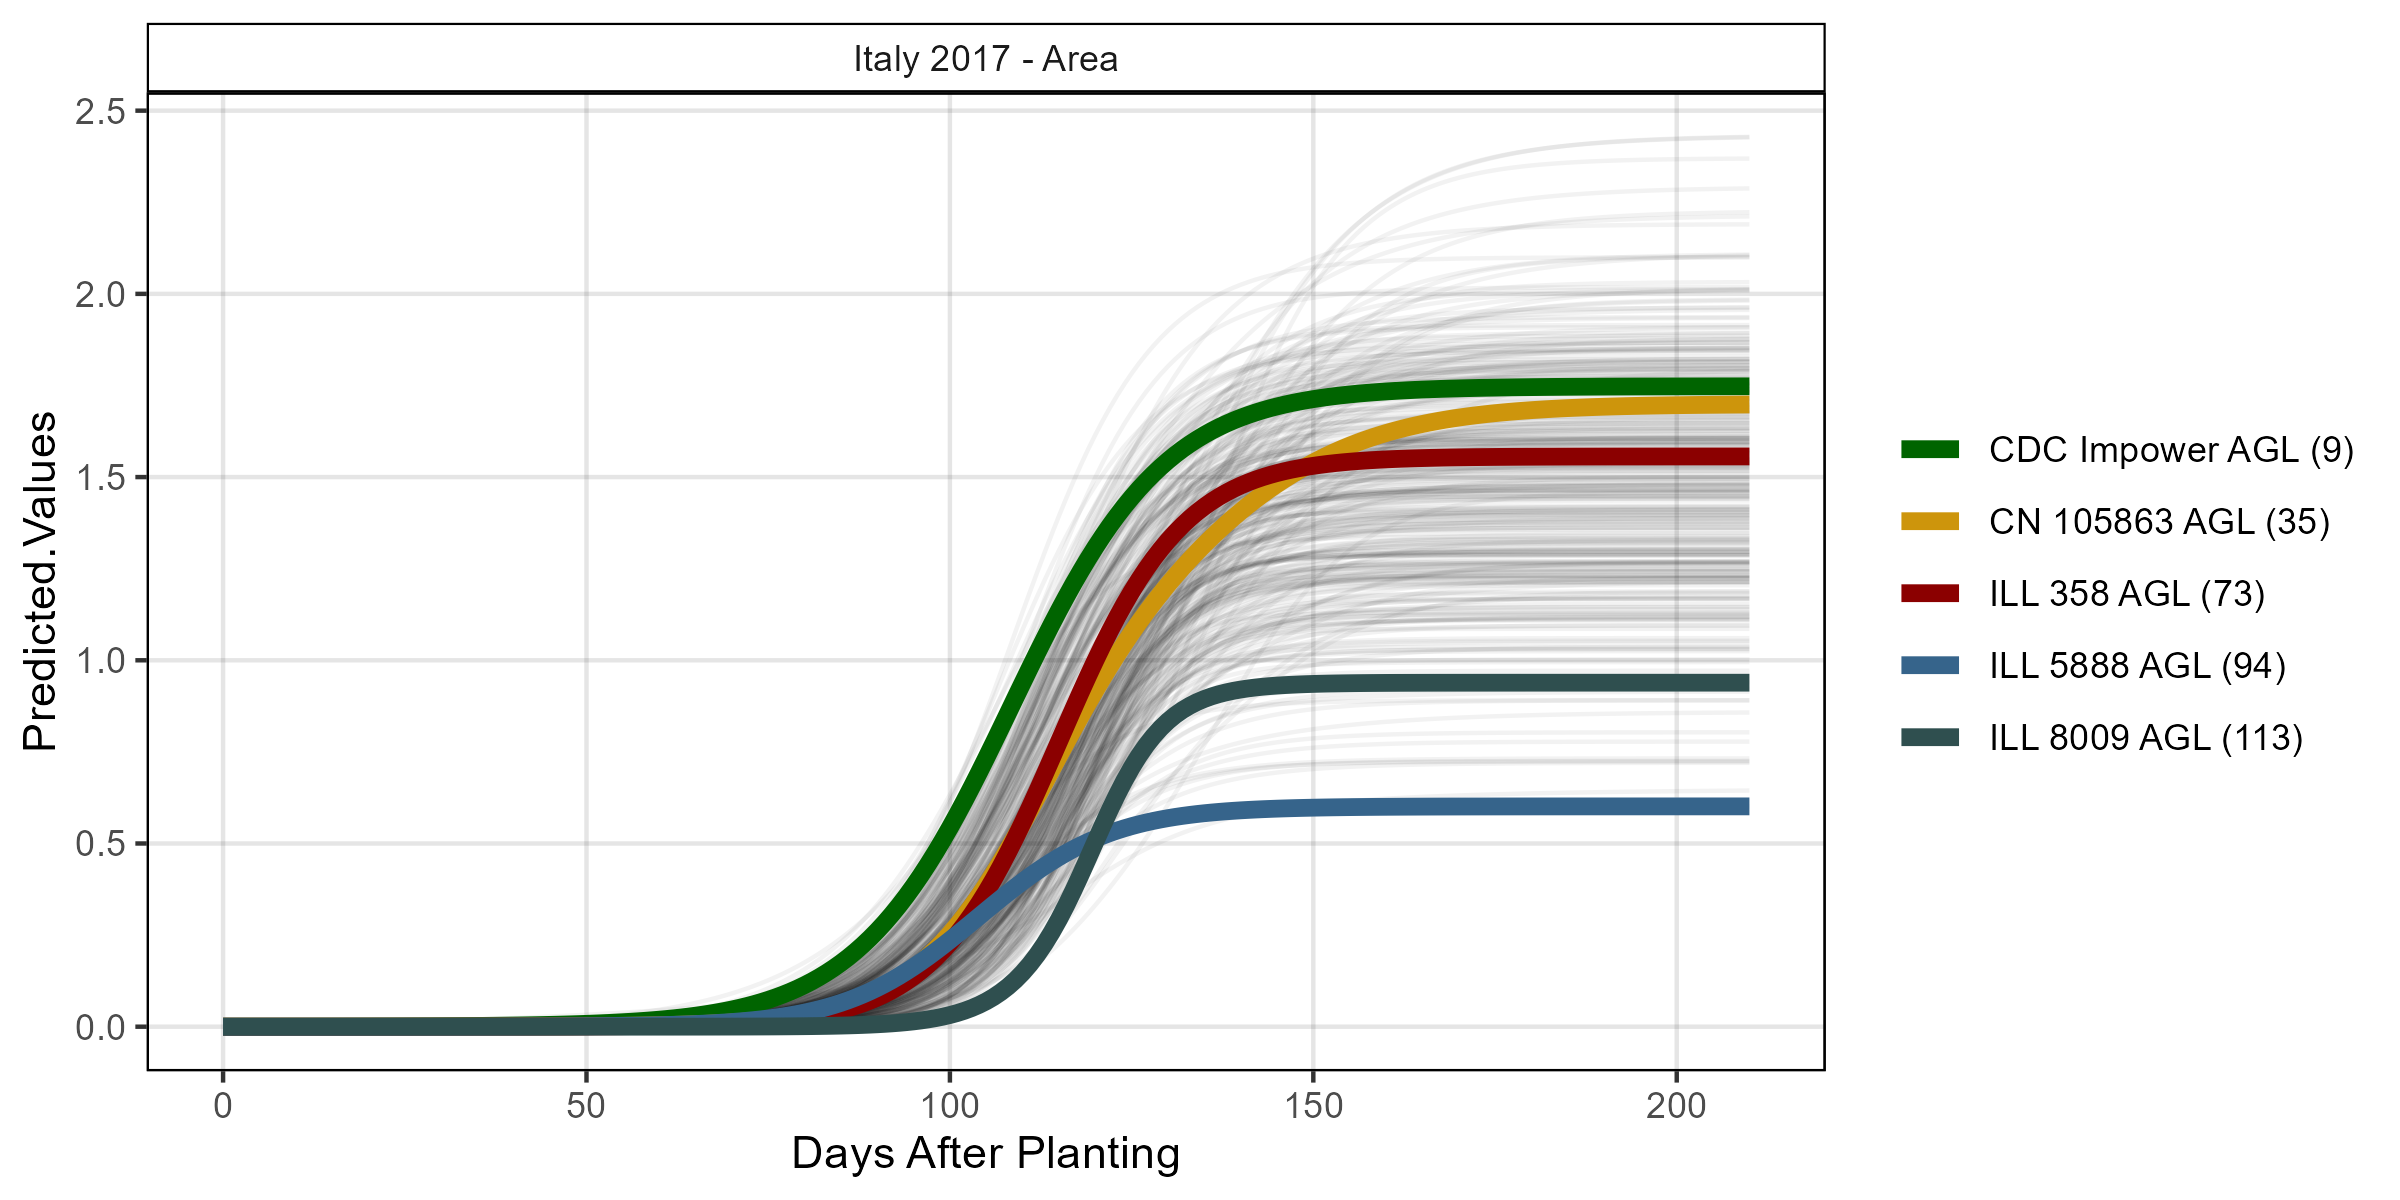
\includegraphics[keepaspectratio]{Additional/ggGrowthCurves_It17_area.png}}

\begin{quote}
\begin{itemize}
\tightlist
\item
  \href{https://derekmichaelwright.github.io/AGILE_LDP_UAV/Additional/ggpGrowthCurves_It17_height.html}{Additional/ggpGrowthCurves\_It17\_height.html}
\end{itemize}
\end{quote}

\pandocbounded{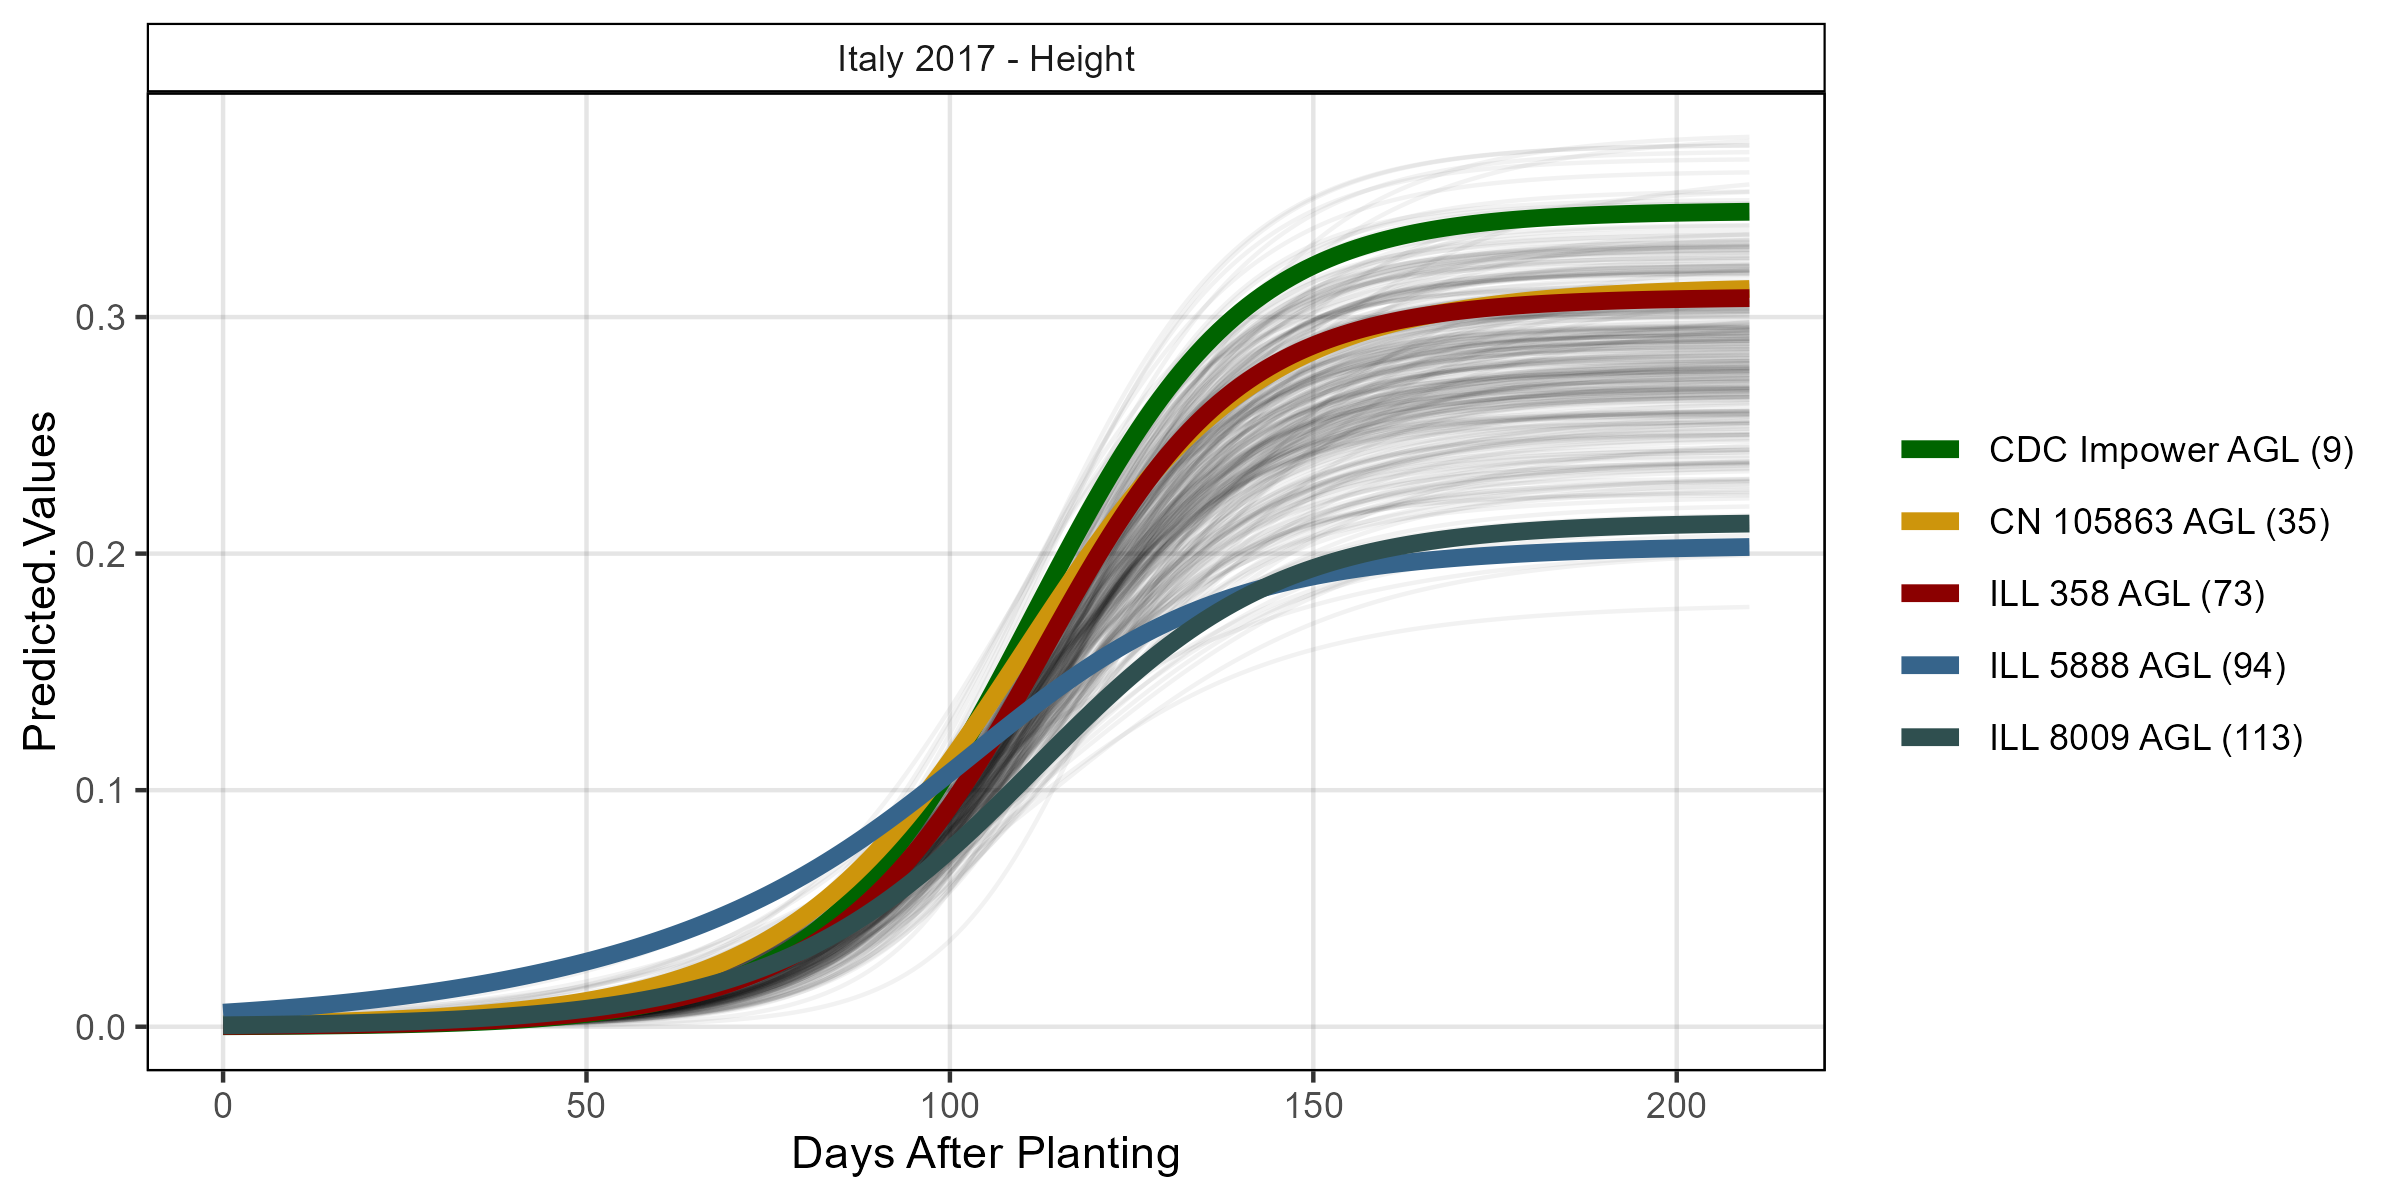
\includegraphics[keepaspectratio]{Additional/ggGrowthCurves_It17_height.png}}

\begin{center}\rule{0.5\linewidth}{0.5pt}\end{center}

\subsection{Rosthern, Canada 2017}\label{rosthern-canada-2017}

\begin{quote}
\begin{itemize}
\tightlist
\item
  \href{https://derekmichaelwright.github.io/AGILE_LDP_UAV/Additional/ggpGrowthCurves_Ro17_volume.html}{Additional/ggpGrowthCurves\_Ro17\_volume.html}
\end{itemize}
\end{quote}

\pandocbounded{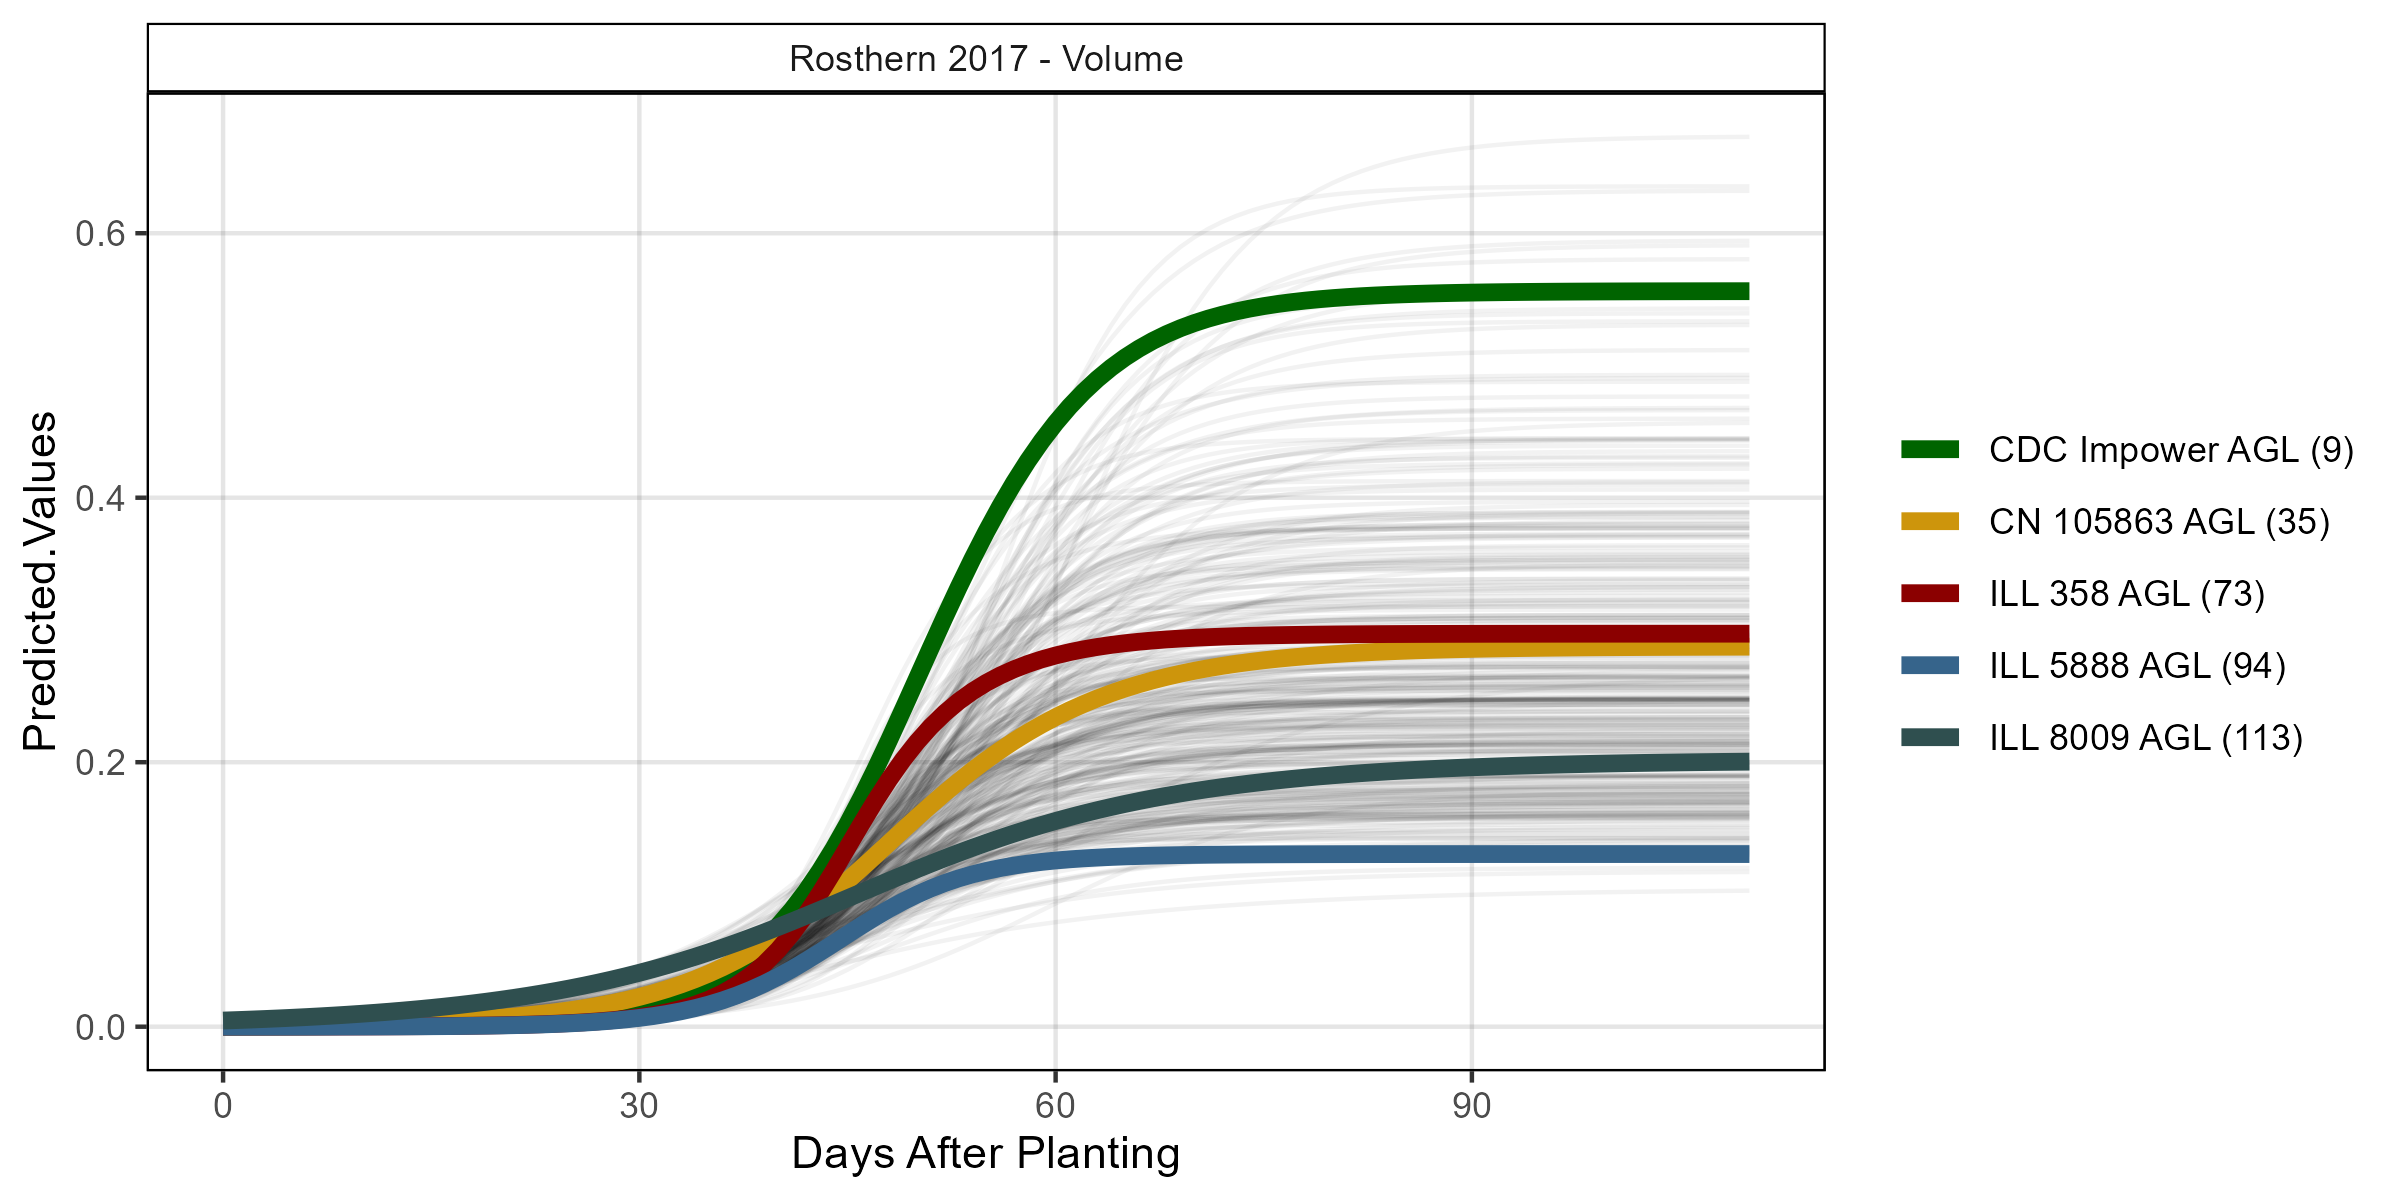
\includegraphics[keepaspectratio]{Additional/ggGrowthCurves_Ro17_volume.png}}

\begin{quote}
\begin{itemize}
\tightlist
\item
  \href{https://derekmichaelwright.github.io/AGILE_LDP_UAV/Additional/ggpGrowthCurves_Ro17_area.html}{Additional/ggpGrowthCurves\_Ro17\_area.html}
\end{itemize}
\end{quote}

\pandocbounded{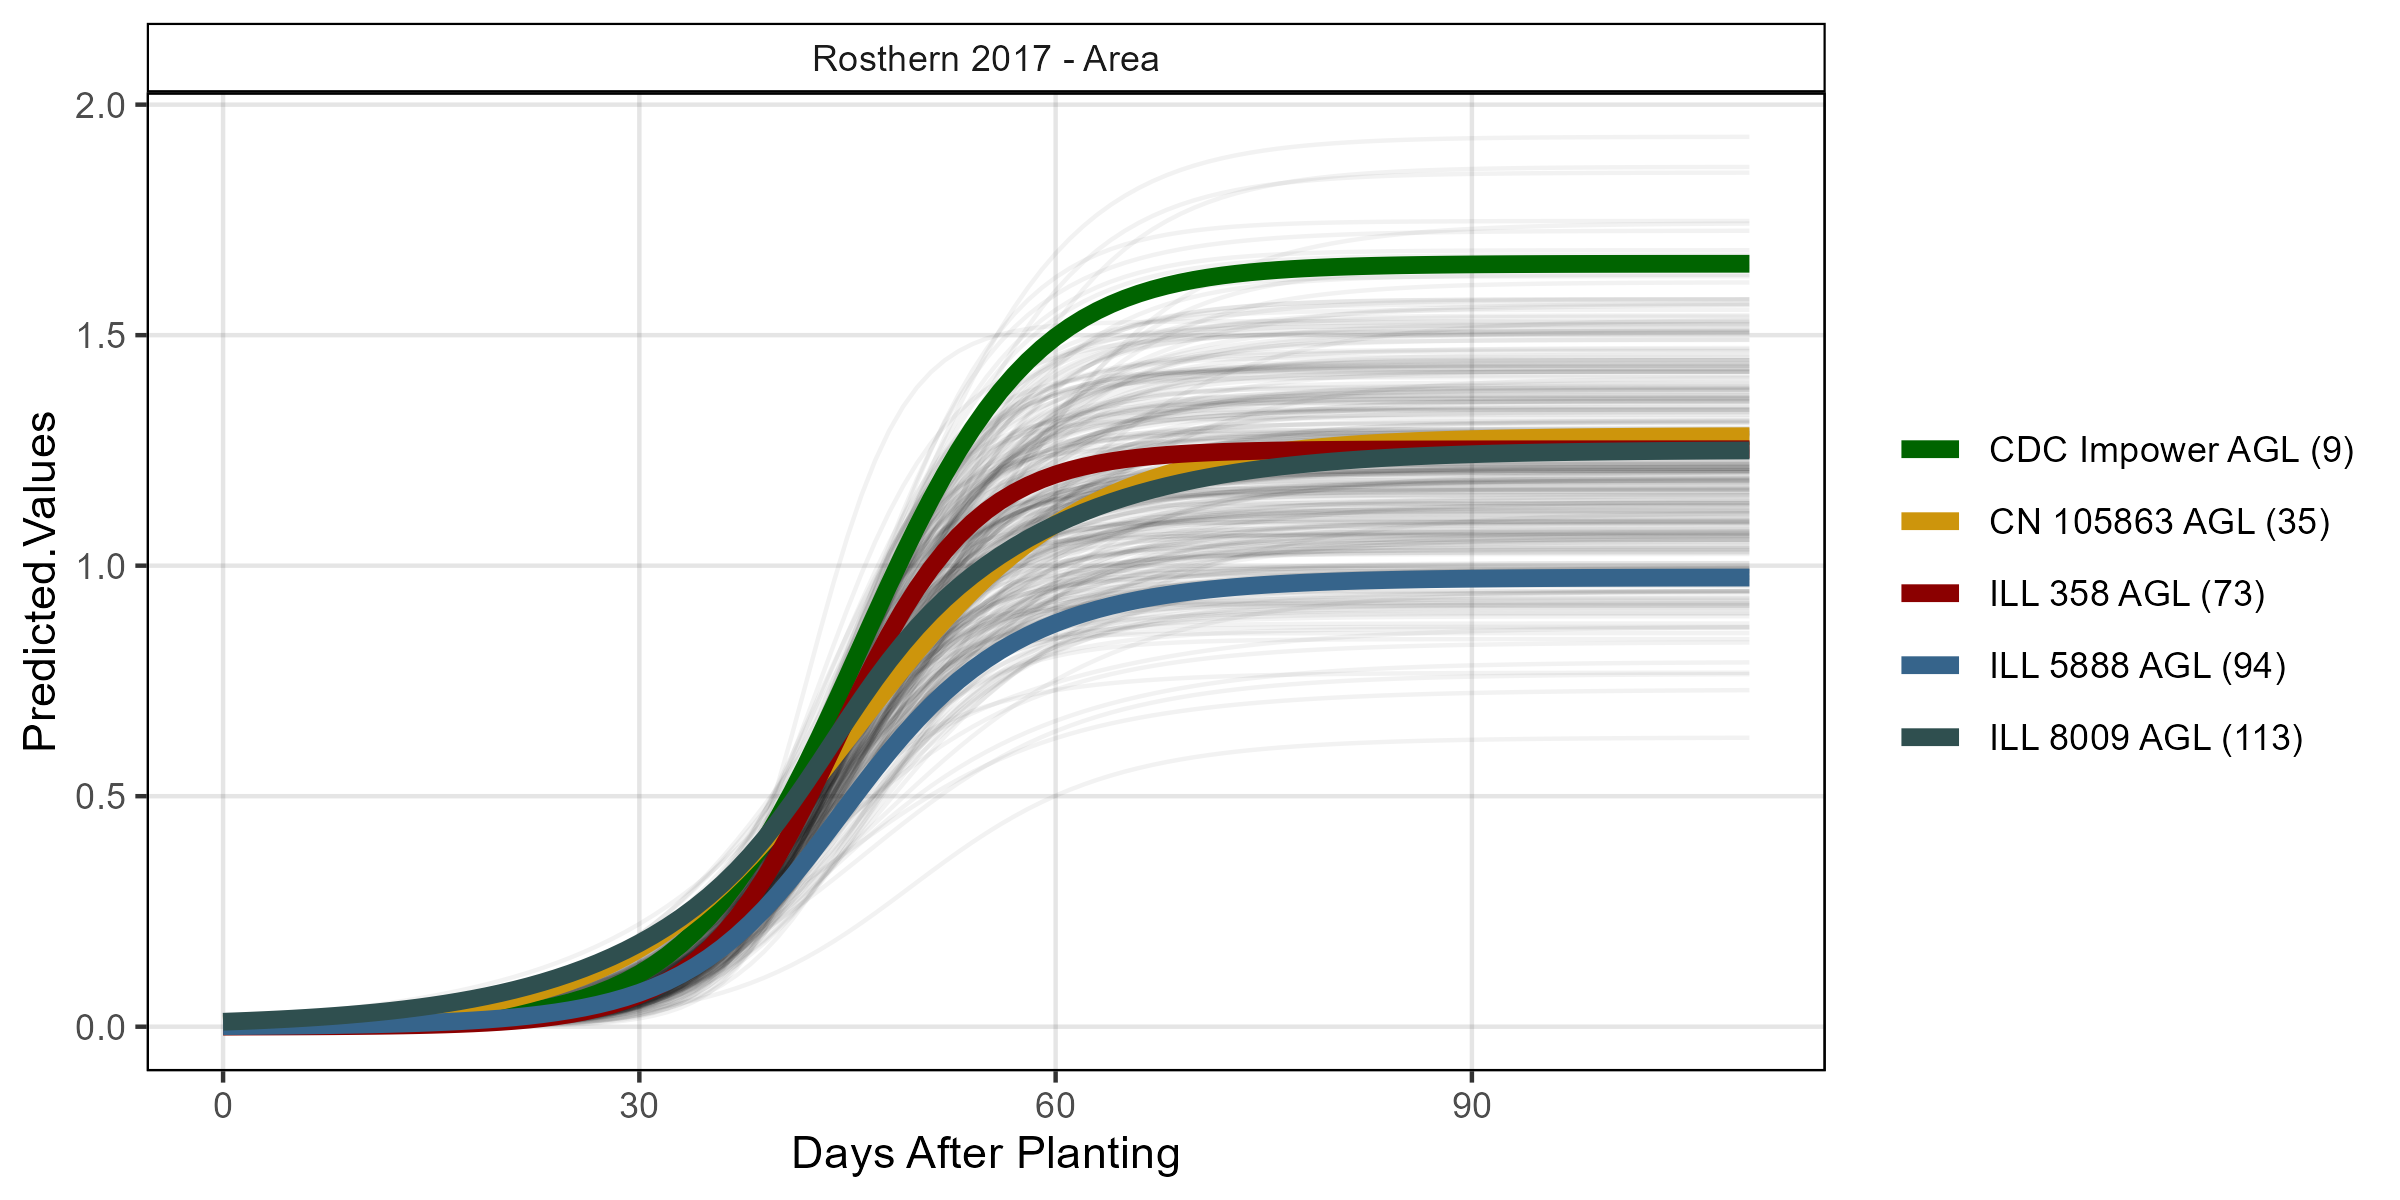
\includegraphics[keepaspectratio]{Additional/ggGrowthCurves_Ro17_area.png}}

\begin{quote}
\begin{itemize}
\tightlist
\item
  \href{https://derekmichaelwright.github.io/AGILE_LDP_UAV/Additional/ggpGrowthCurves_Ro17_height.html}{Additional/ggpGrowthCurves\_Ro17\_height.html}
\end{itemize}
\end{quote}

\pandocbounded{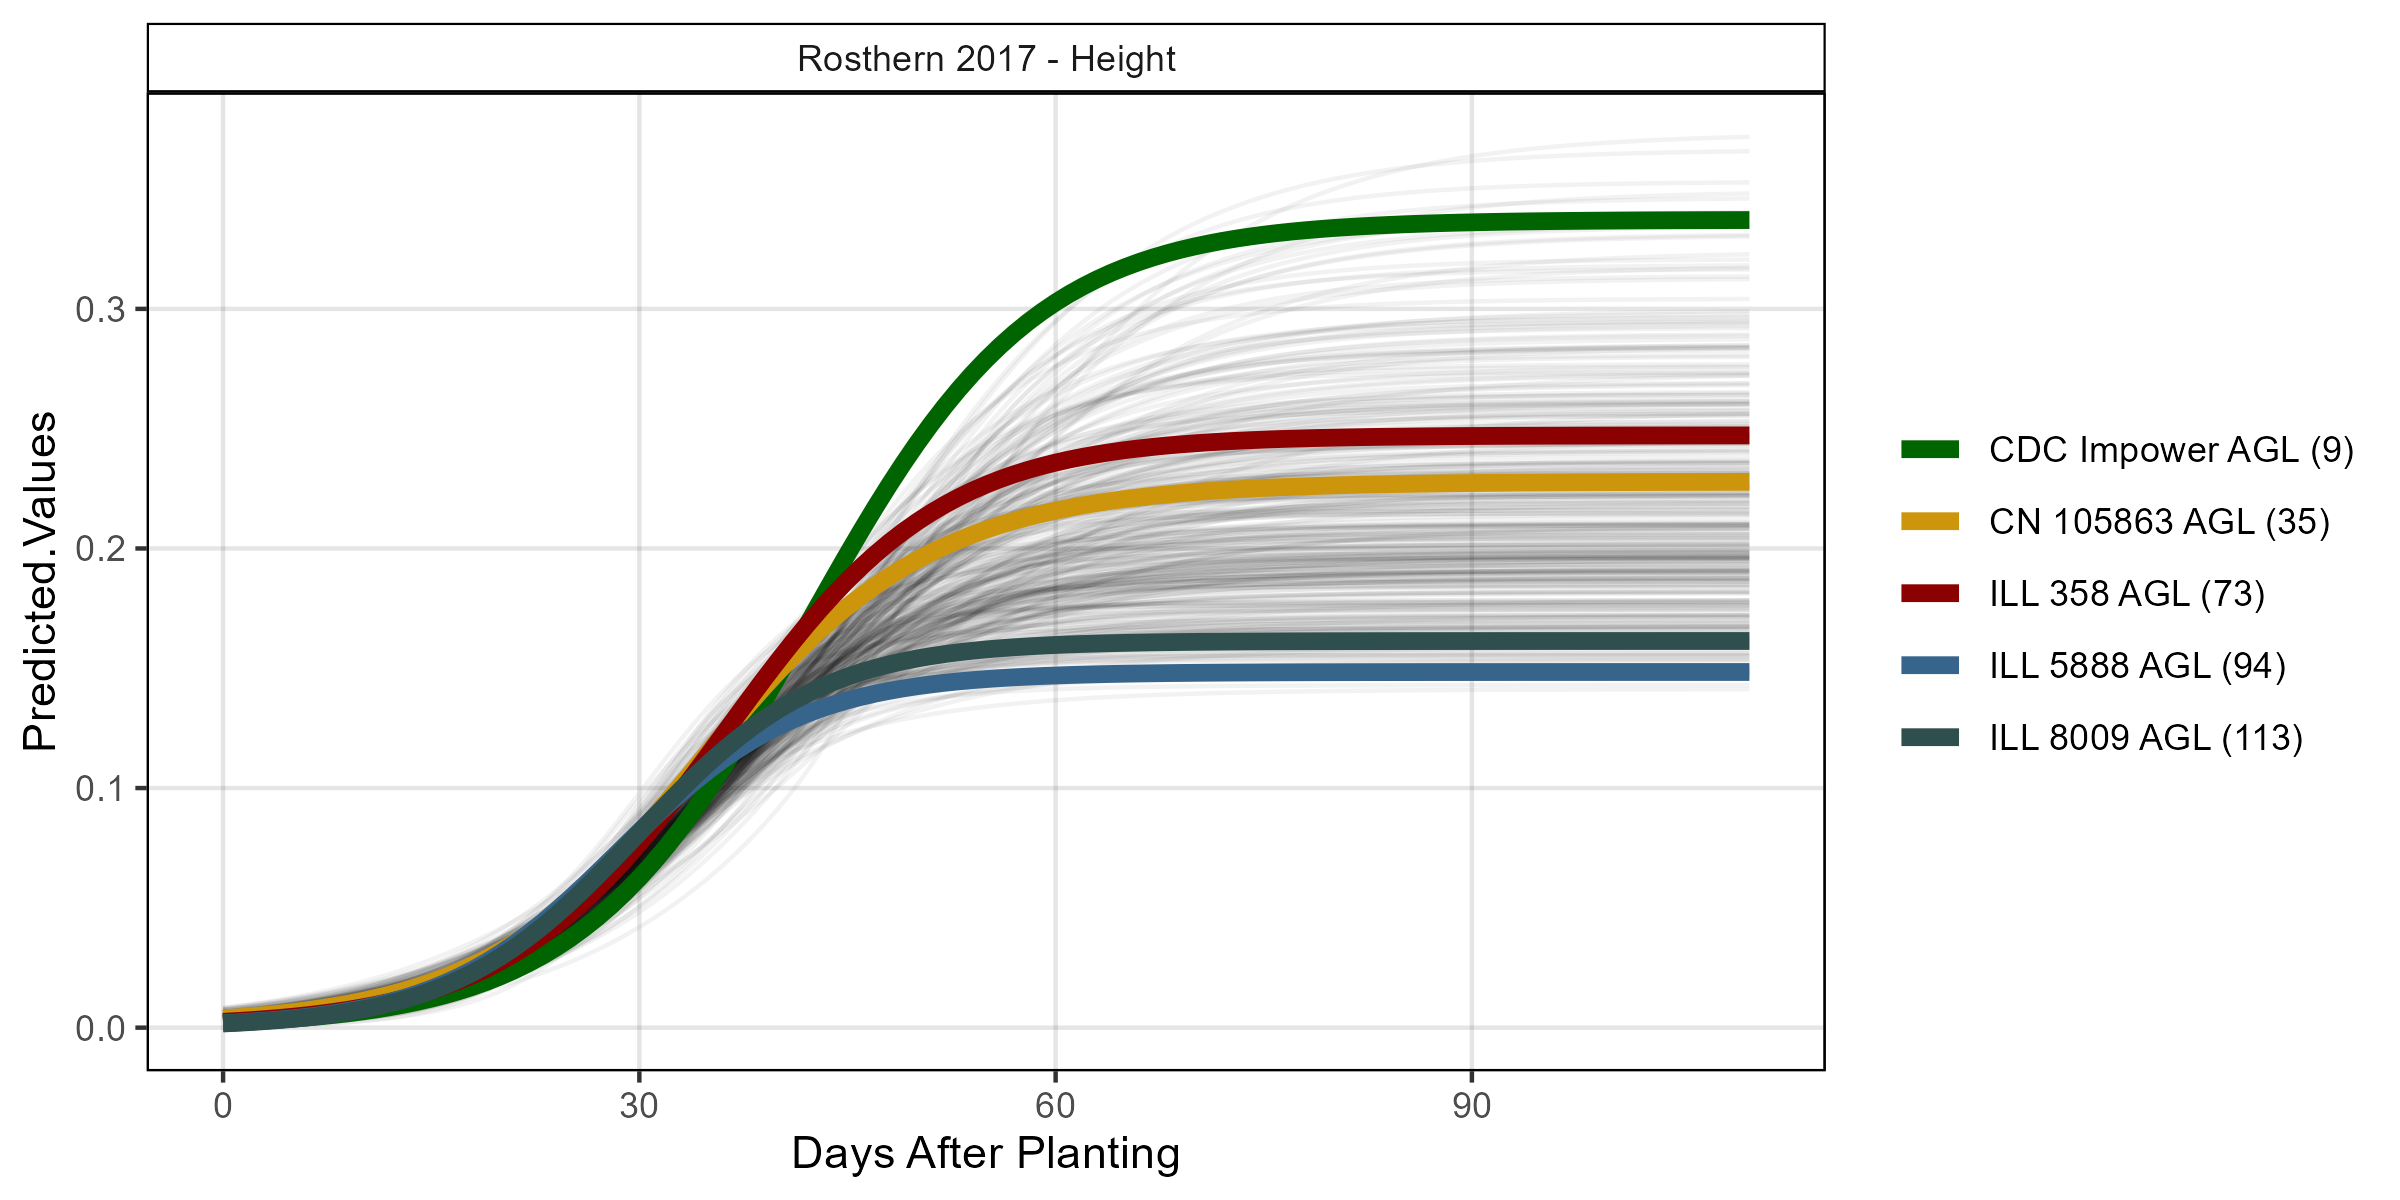
\includegraphics[keepaspectratio]{Additional/ggGrowthCurves_Ro17_height.png}}

\begin{center}\rule{0.5\linewidth}{0.5pt}\end{center}

\subsection{Sutherland, Canada 2017}\label{sutherland-canada-2017}

\href{https://derekmichaelwright.github.io/AGILE_LDP_UAV/Additional/ggpGrowthCurves_Su17_volume.html}{Additional/ggpGrowthCurves\_Su17\_volume.html}

\pandocbounded{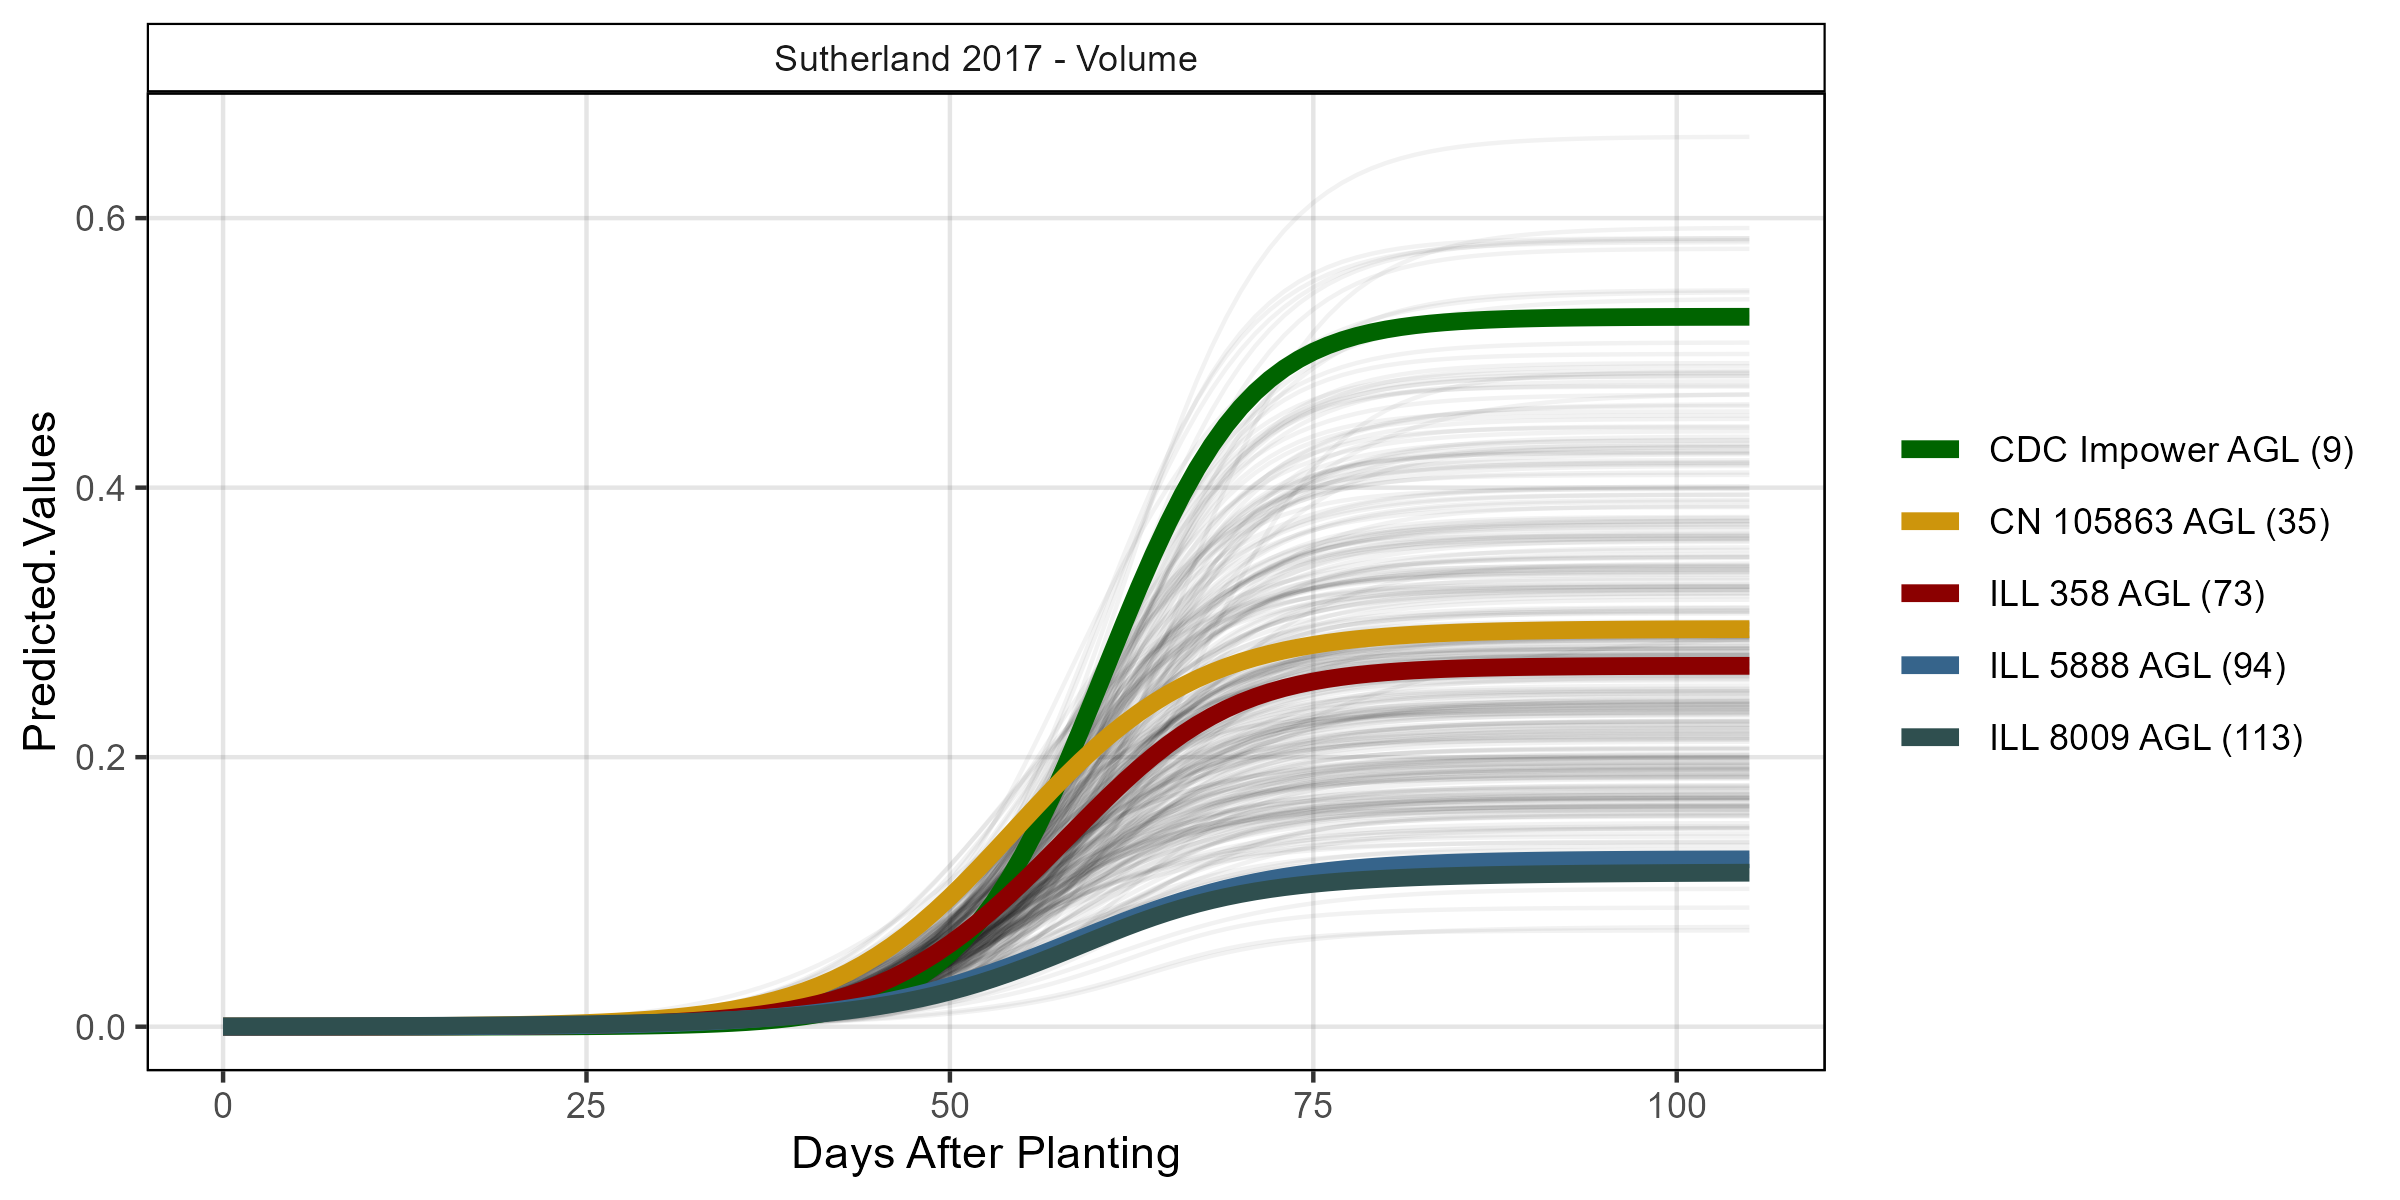
\includegraphics[keepaspectratio]{Additional/ggGrowthCurves_Su17_volume.png}}

\href{https://derekmichaelwright.github.io/AGILE_LDP_UAV/Additional/ggpGrowthCurves_Su17_area.html}{Additional/ggpGrowthCurves\_Su17\_area.html}

\pandocbounded{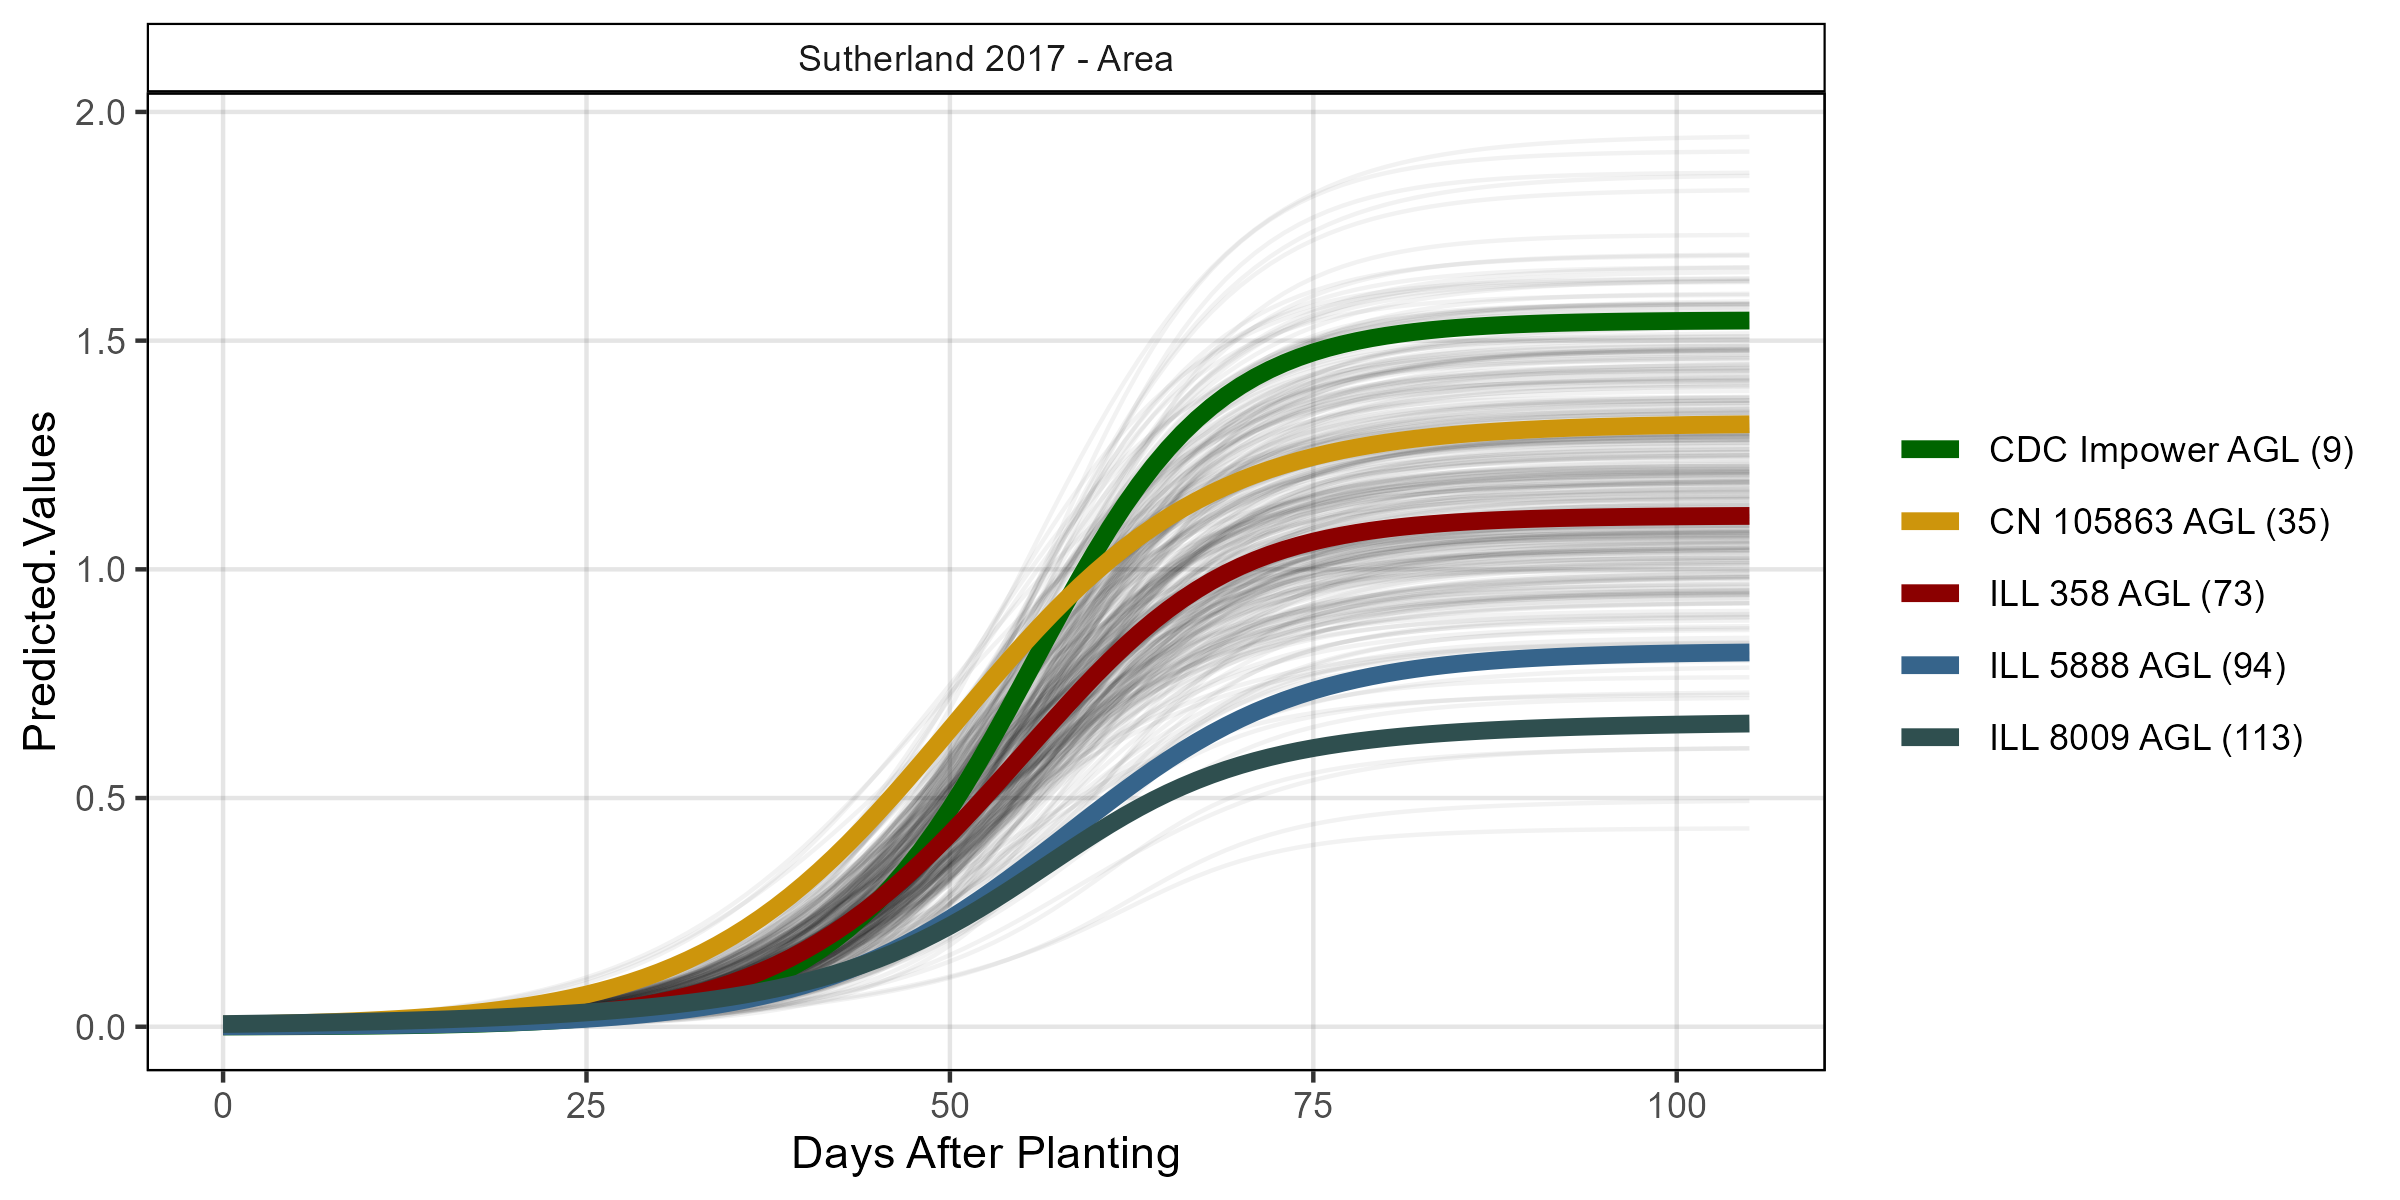
\includegraphics[keepaspectratio]{Additional/ggGrowthCurves_Su17_area.png}}

\href{https://derekmichaelwright.github.io/AGILE_LDP_UAV/Additional/ggpGrowthCurves_Su17_height.html}{Additional/ggpGrowthCurves\_Su17\_height.html}

\pandocbounded{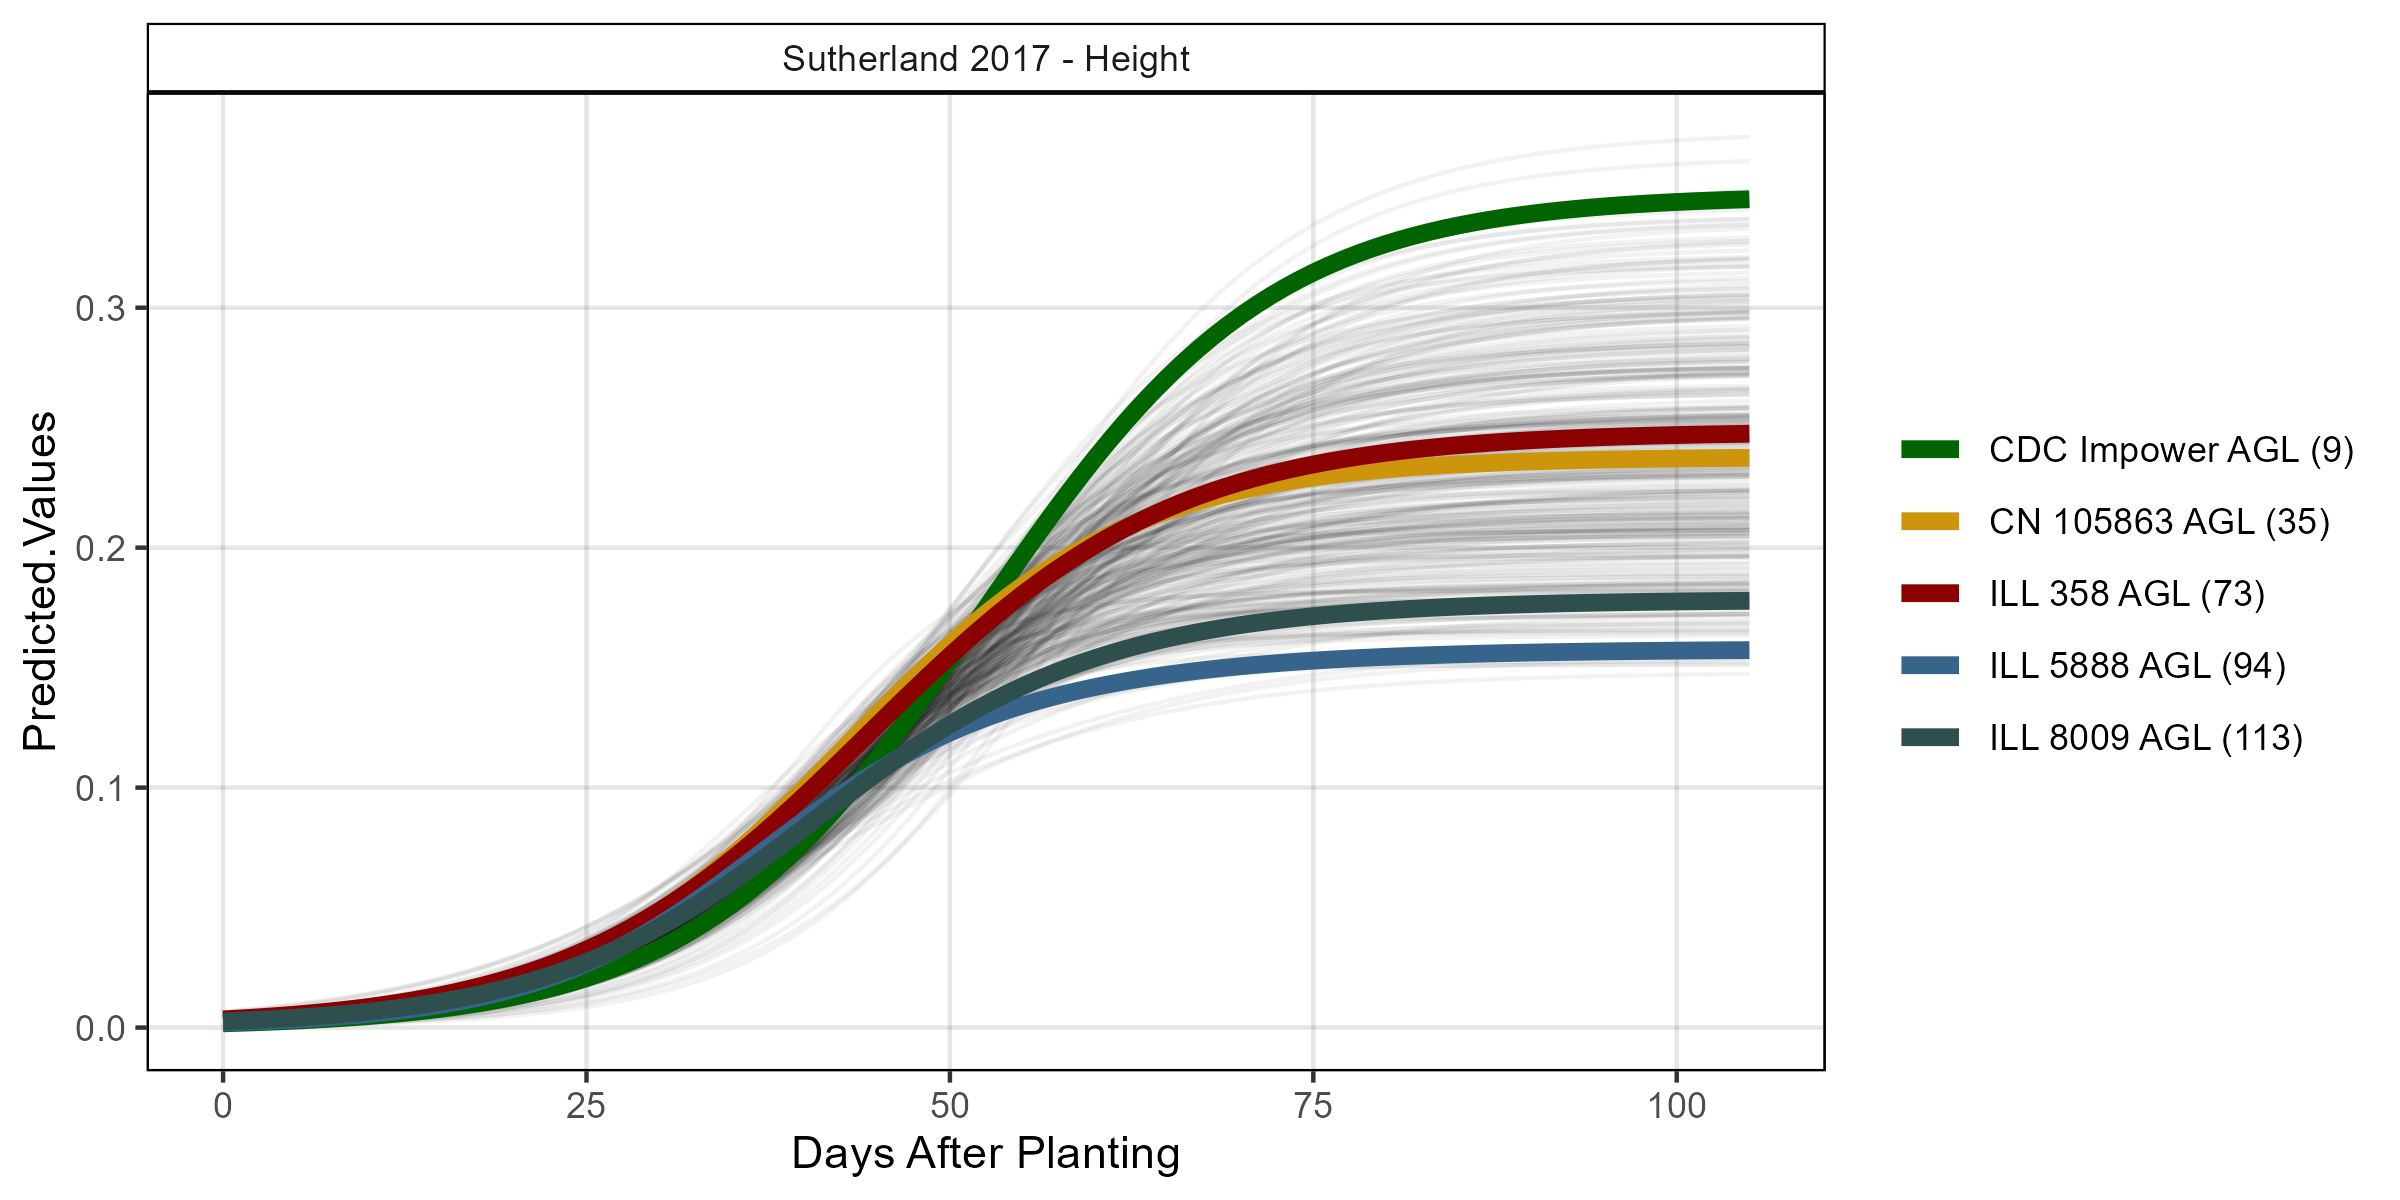
\includegraphics[keepaspectratio]{Additional/ggGrowthCurves_Su17_height.png}}

\begin{center}\rule{0.5\linewidth}{0.5pt}\end{center}

\subsection{Sutherland, Canada 2018}\label{sutherland-canada-2018}

\begin{center}\rule{0.5\linewidth}{0.5pt}\end{center}

\section{Figures}\label{figures}

\subsection{Figure 1}\label{figure-1}

\pandocbounded{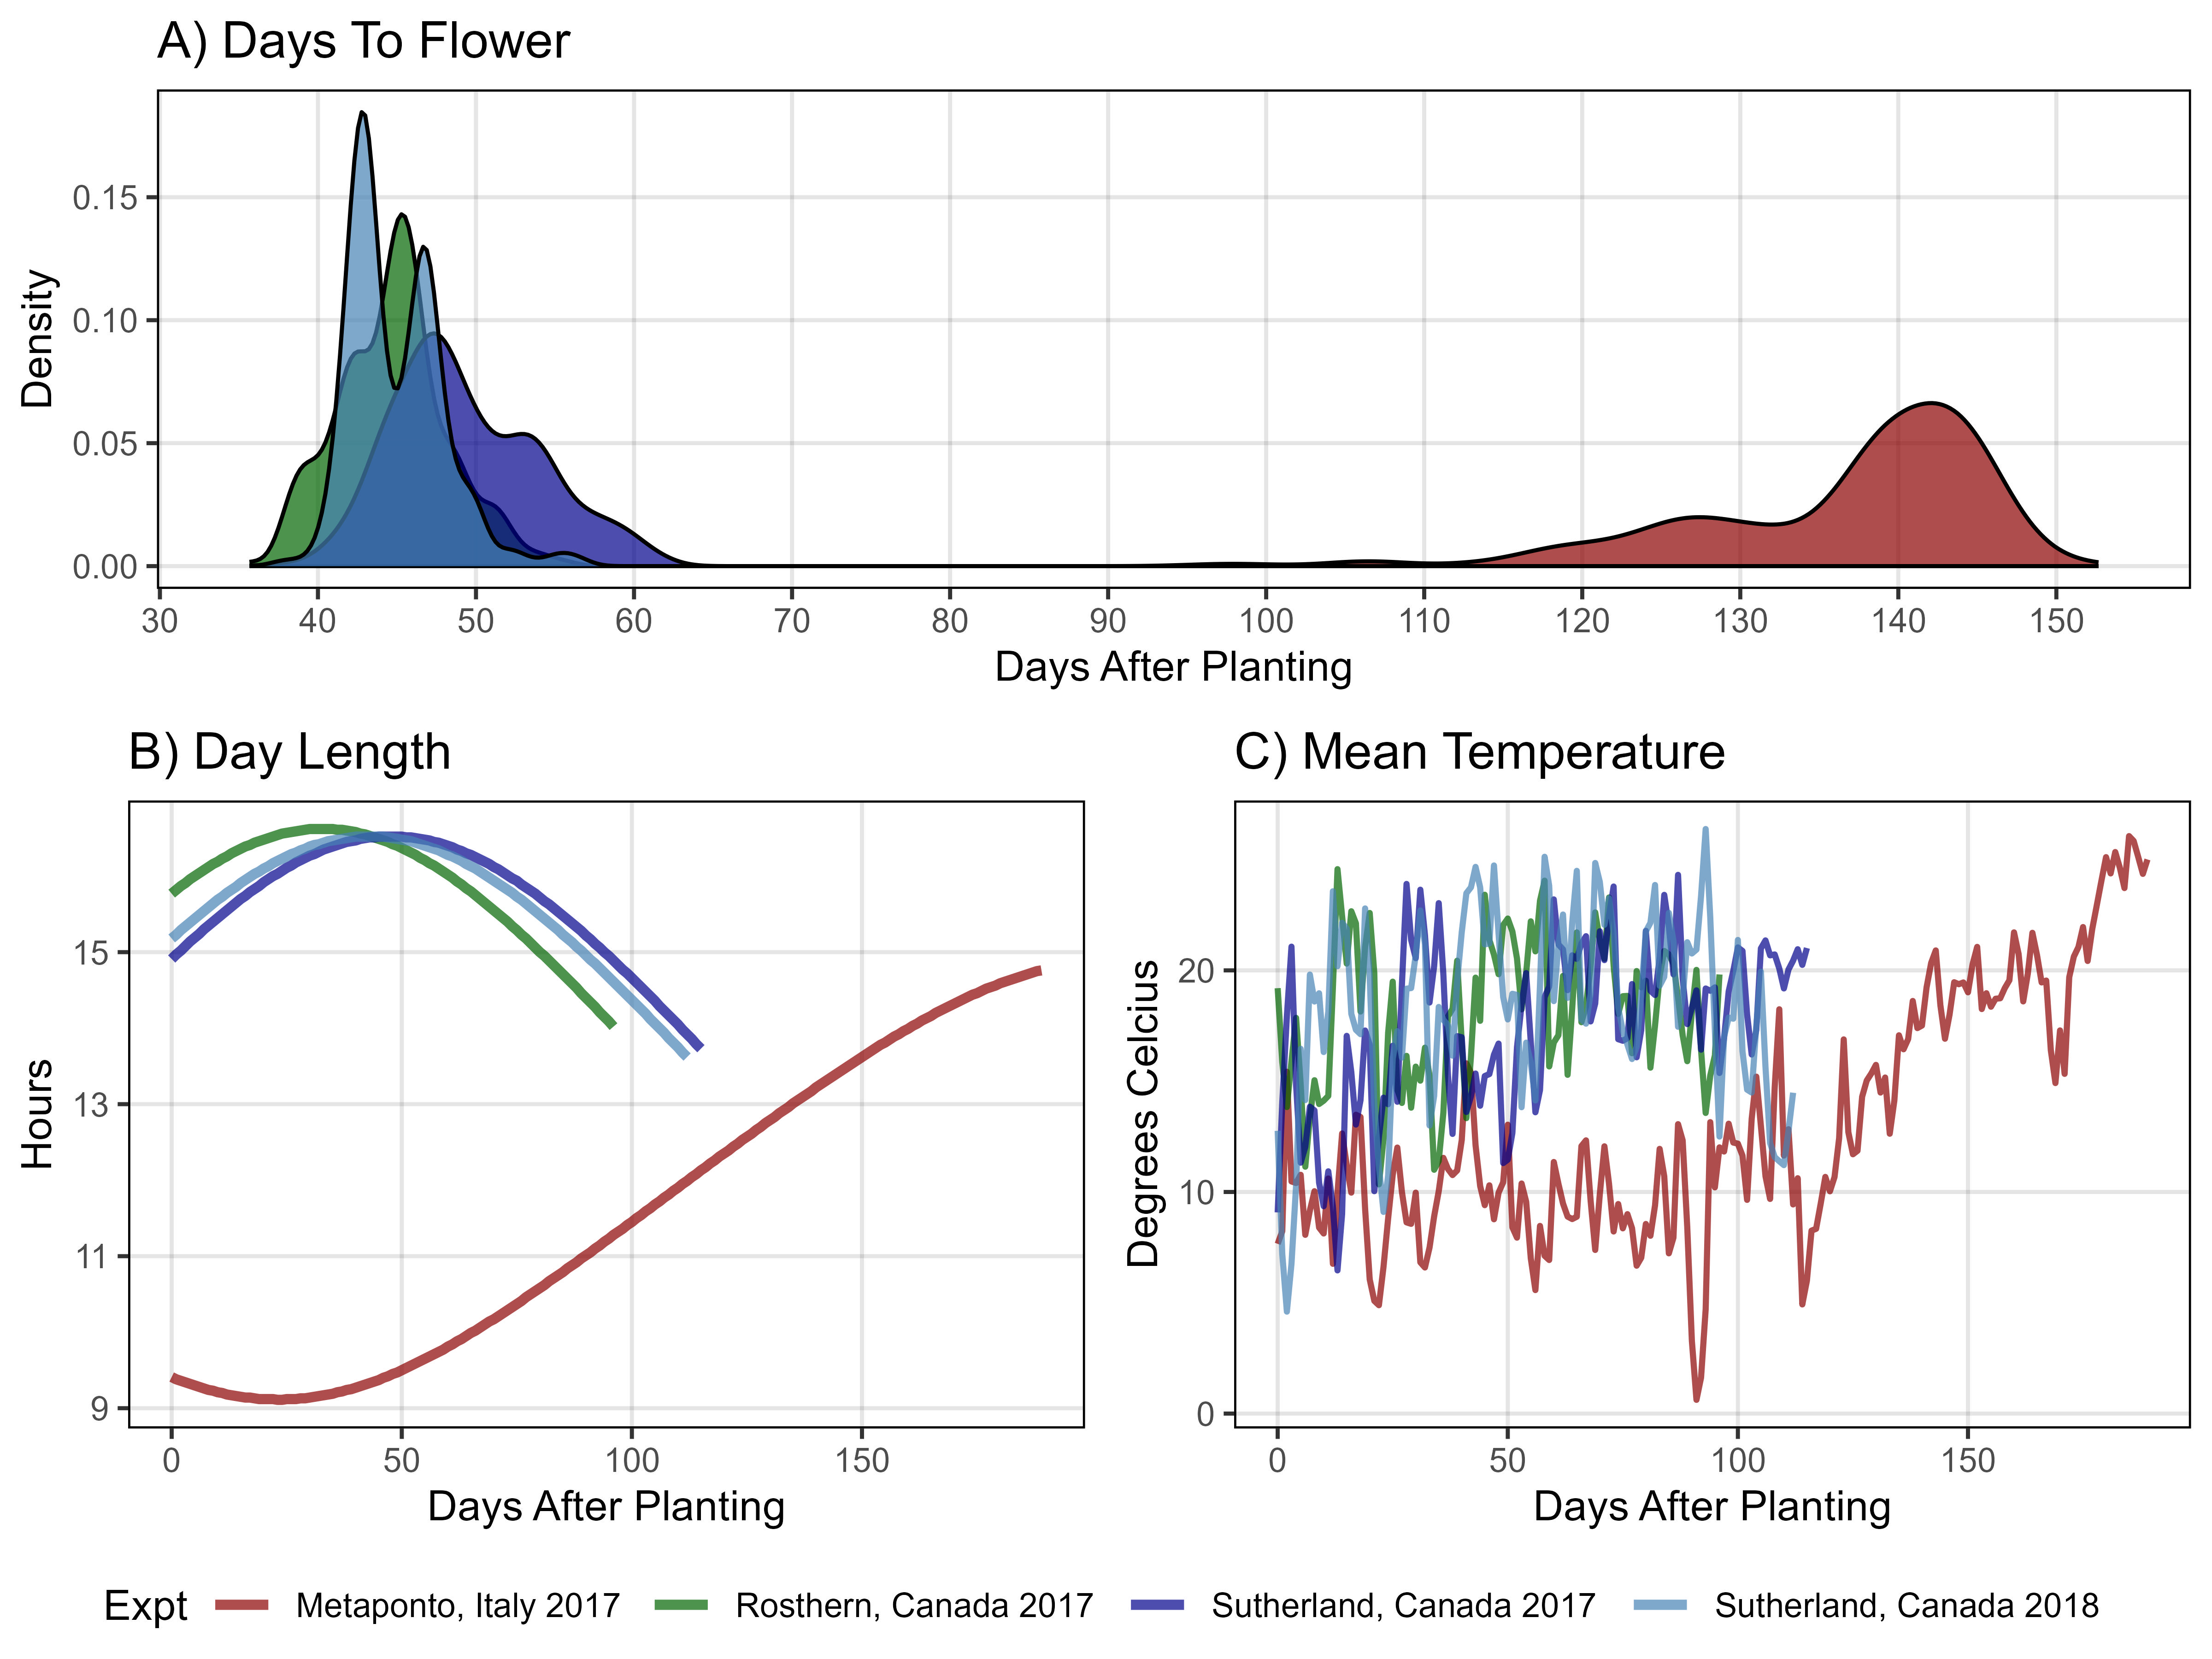
\includegraphics[keepaspectratio]{Figure_01.jpg}}

\begin{center}\rule{0.5\linewidth}{0.5pt}\end{center}

\subsection{Figure 2}\label{figure-2}

\pandocbounded{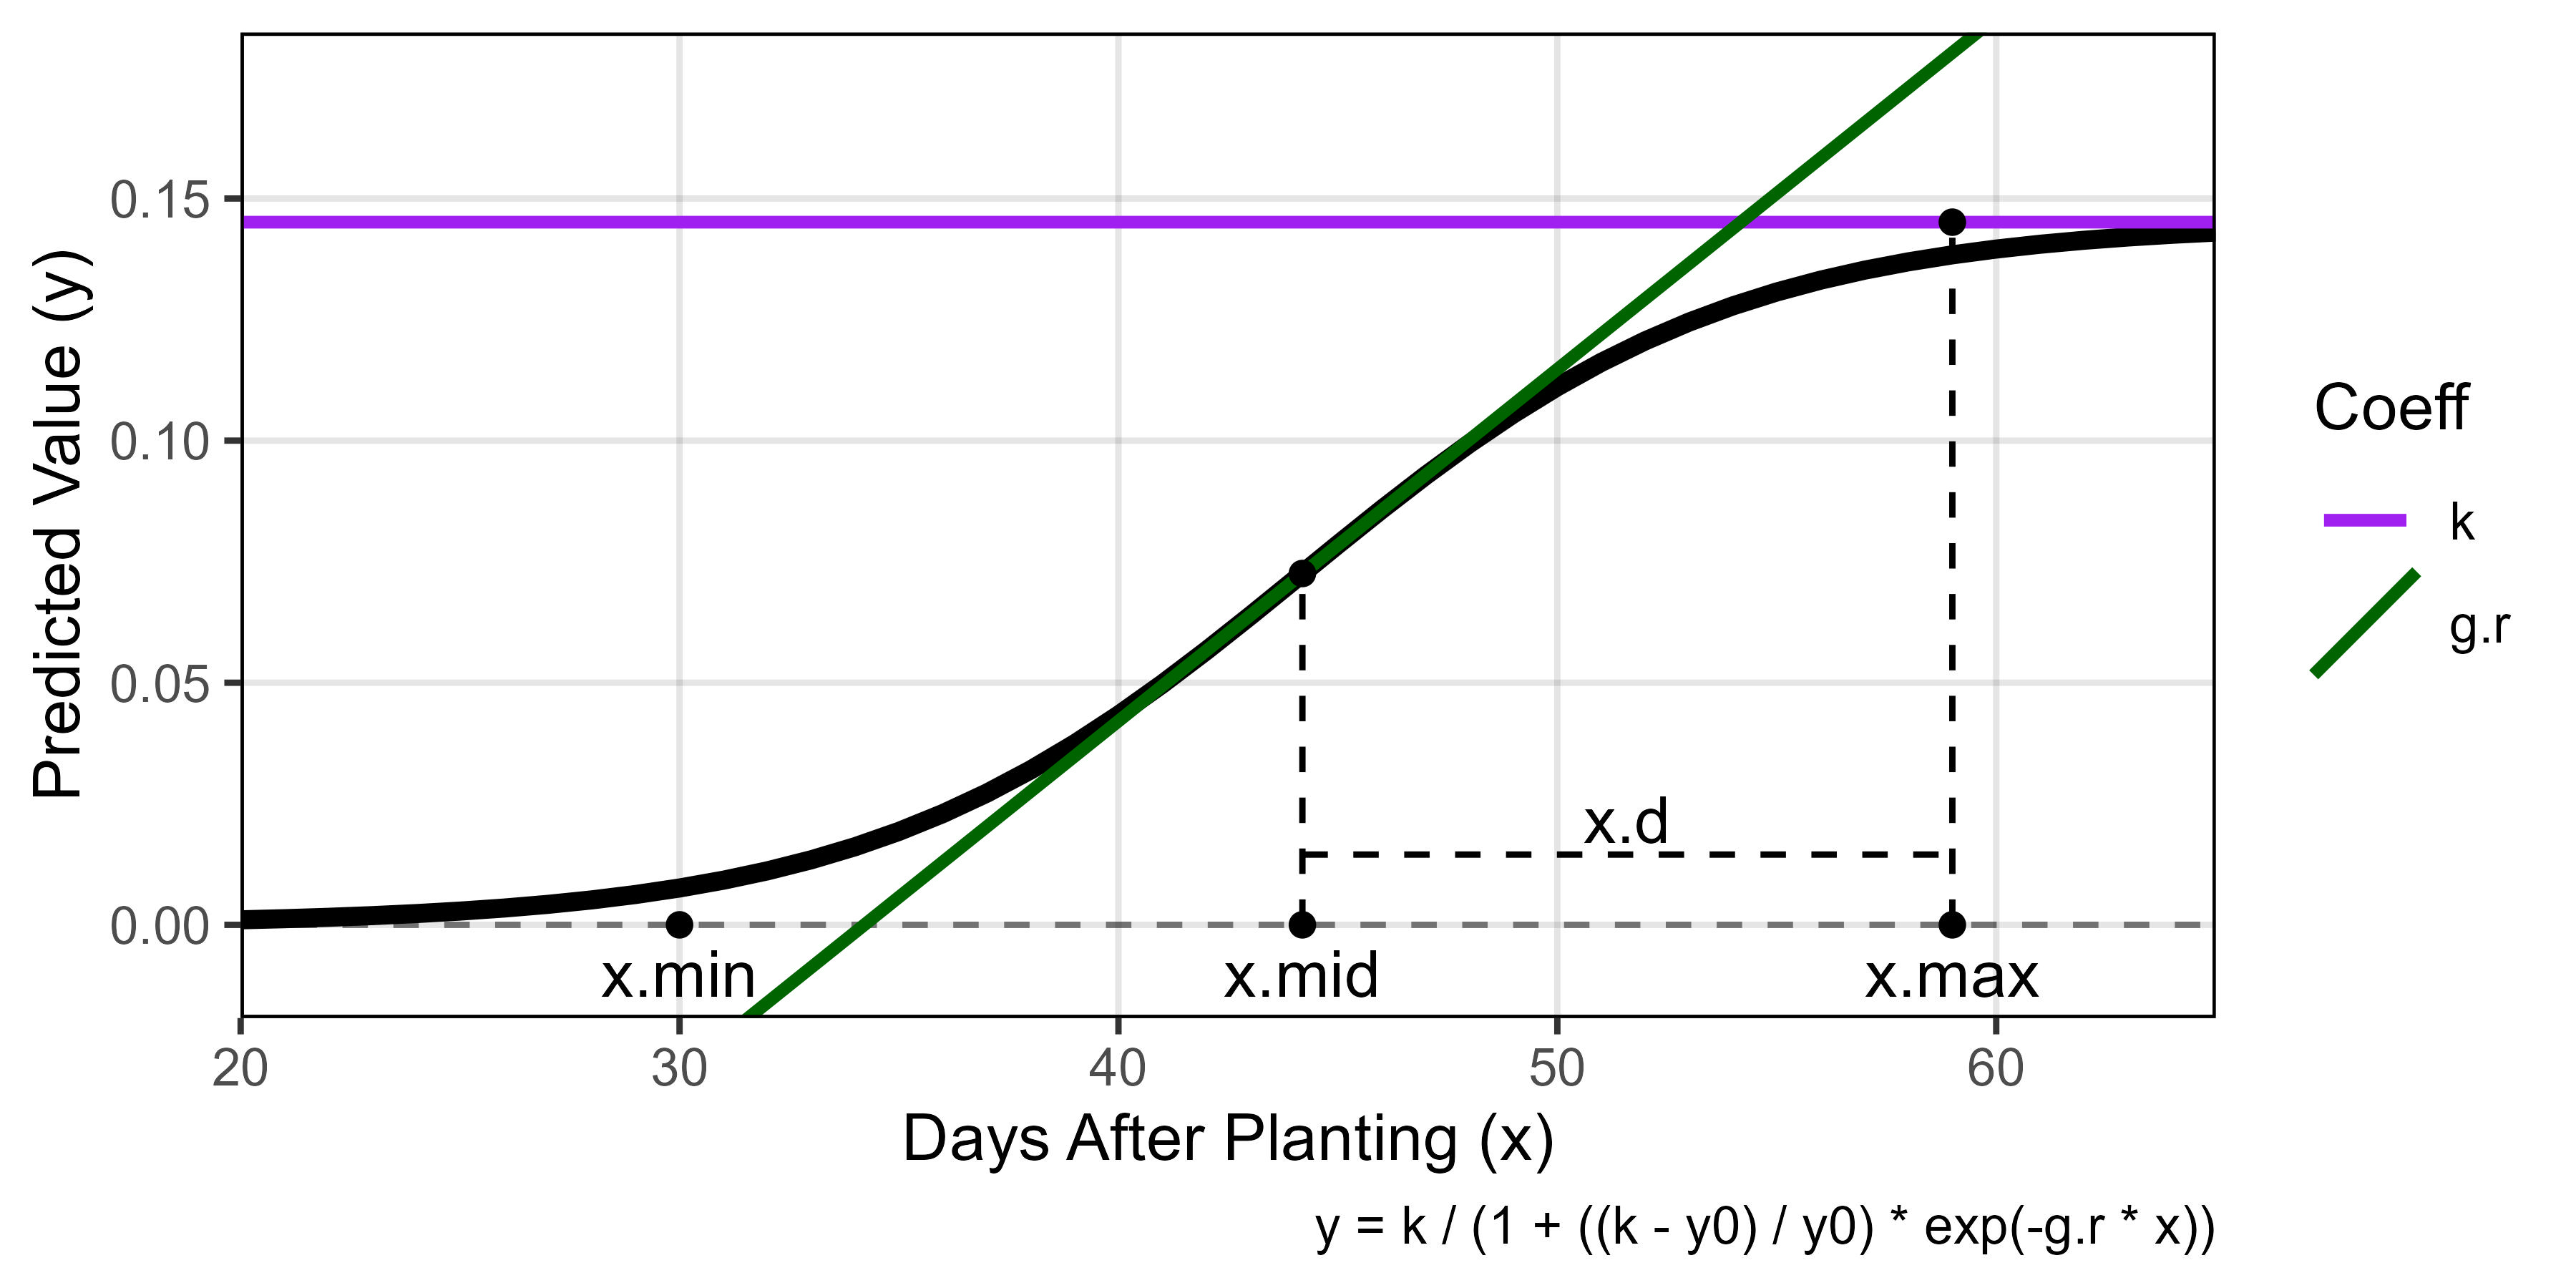
\includegraphics[keepaspectratio]{Figure_02.jpg}}

\begin{center}\rule{0.5\linewidth}{0.5pt}\end{center}

\subsection{Figure 3}\label{figure-3}

\pandocbounded{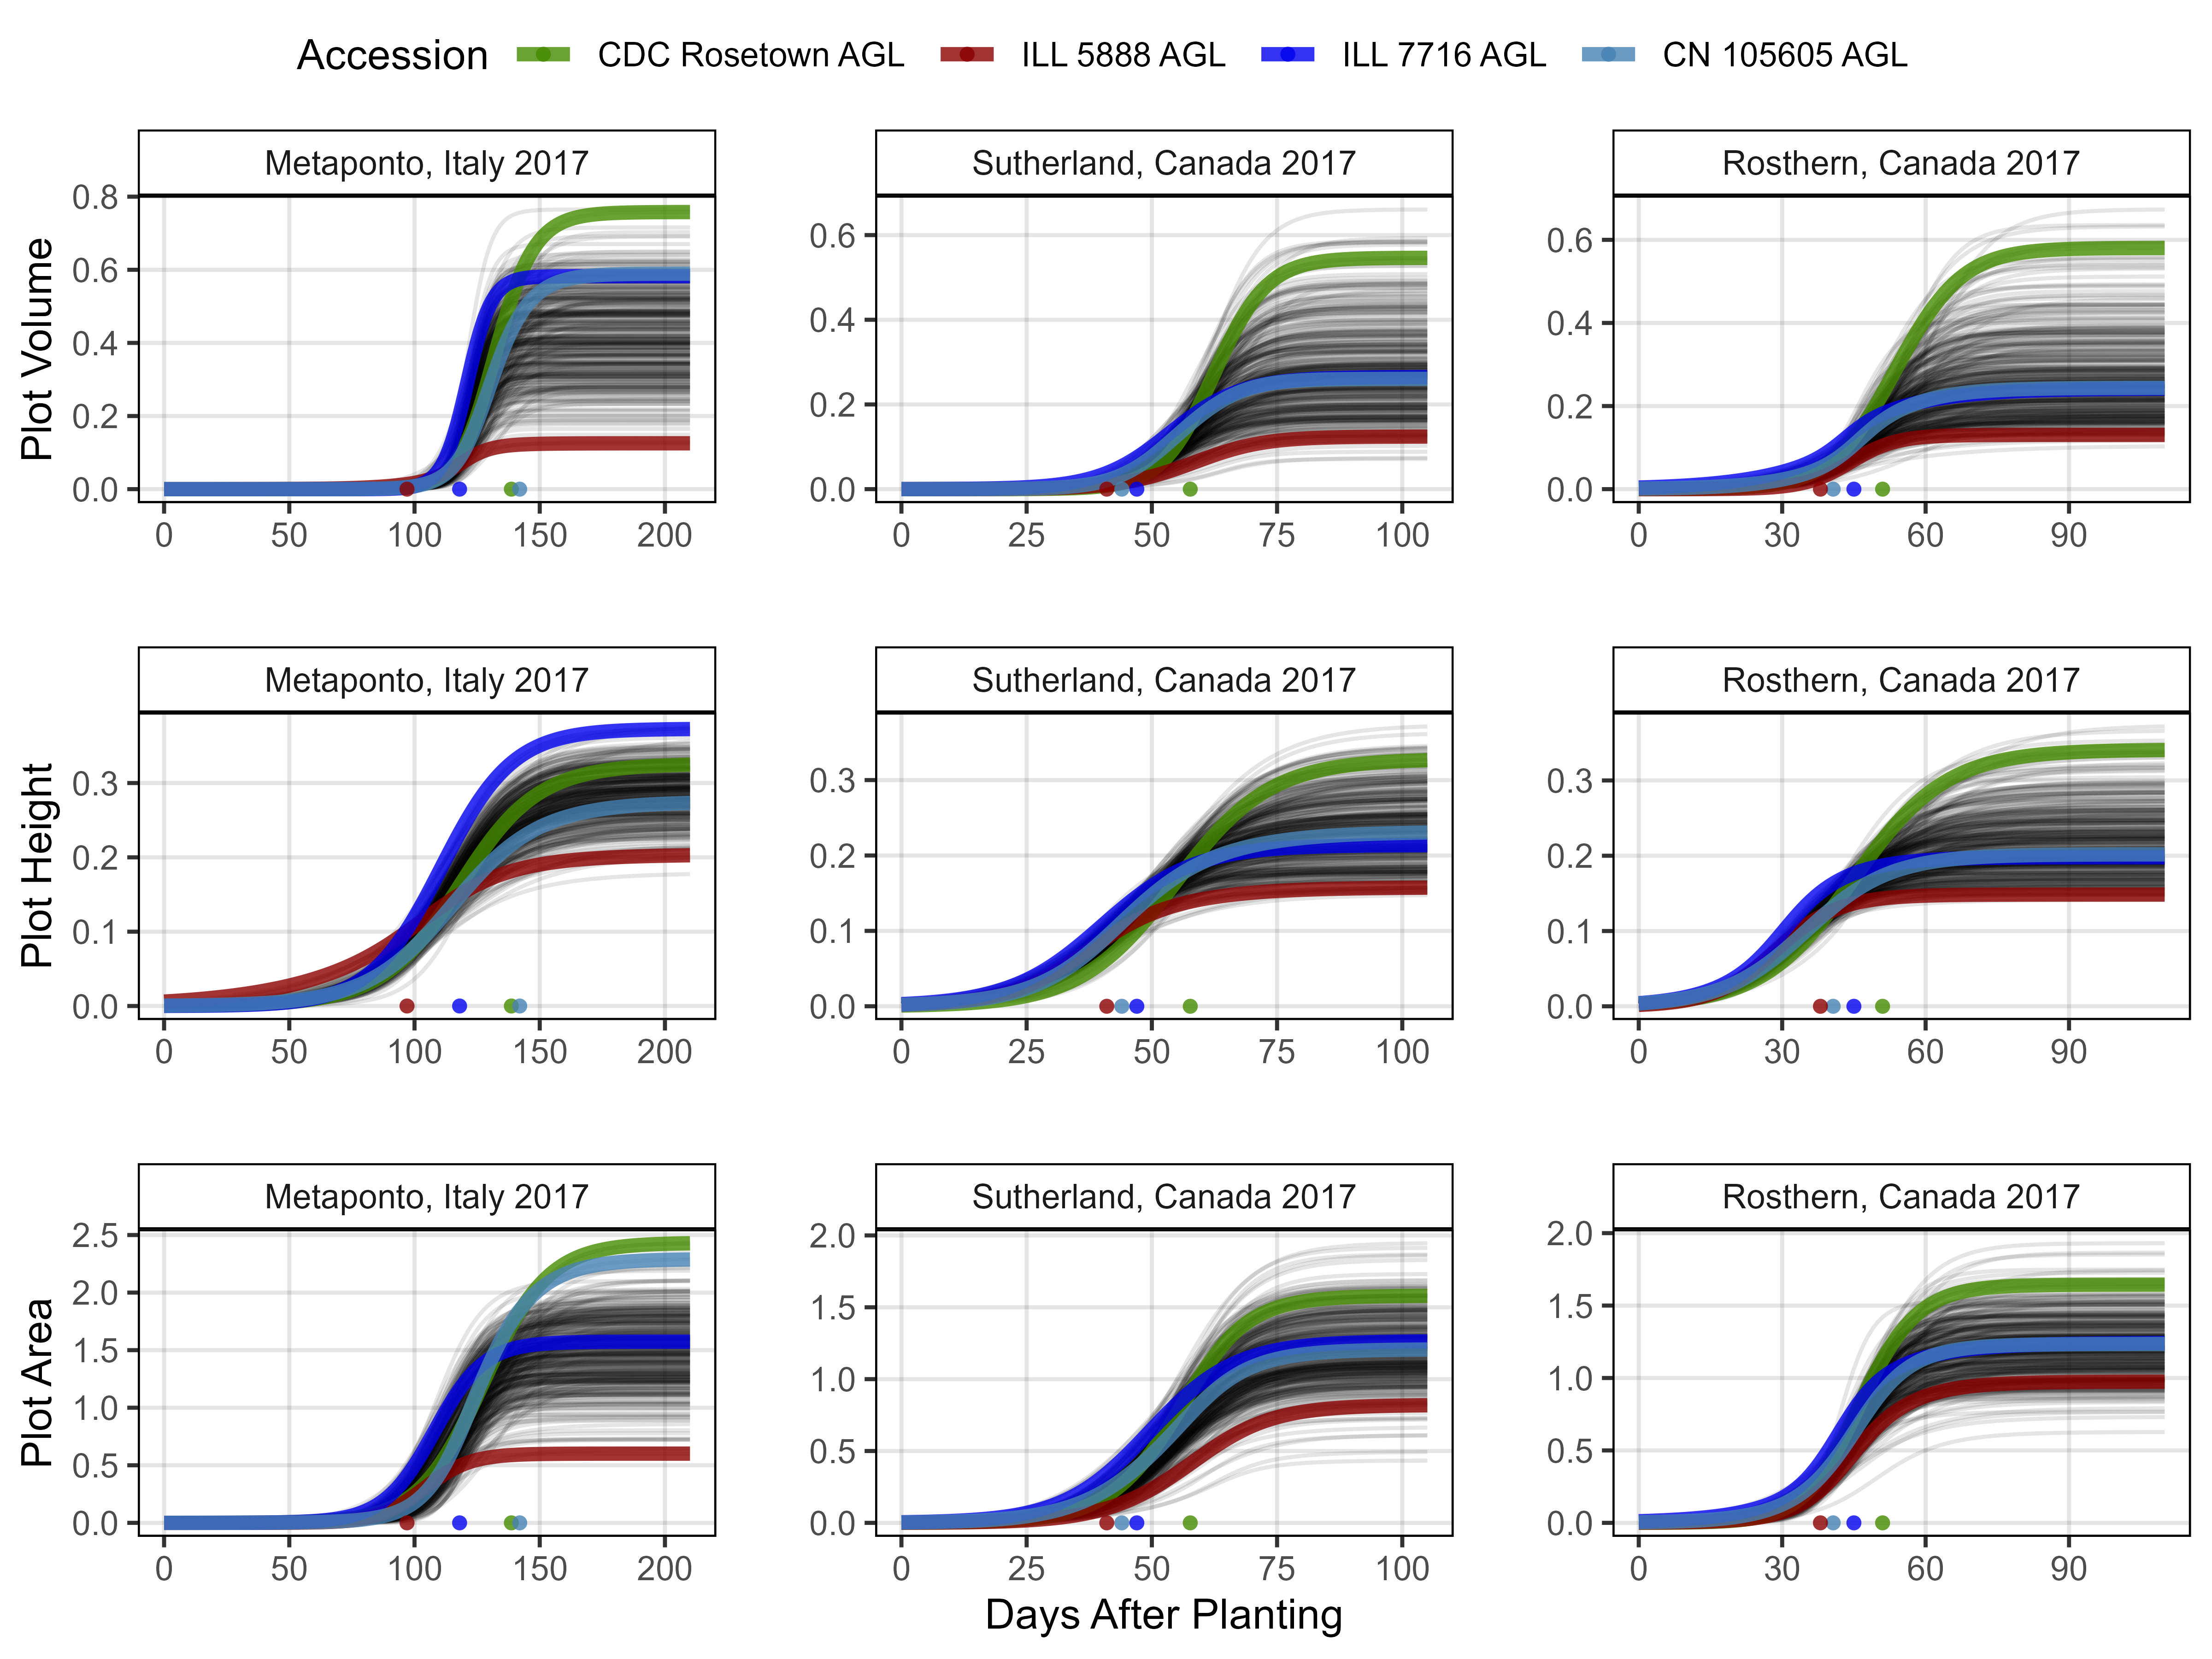
\includegraphics[keepaspectratio]{Figure_03.jpg}}

\begin{center}\rule{0.5\linewidth}{0.5pt}\end{center}

\pagebreak

\subsection{Figure 4}\label{figure-4}

\begin{quote}
\begin{itemize}
\tightlist
\item
  \href{https://derekmichaelwright.github.io/AGILE_LDP_UAV/Additional/Figure_04_A.html}{Additional/Figure\_04\_A.html}
\item
  \href{https://derekmichaelwright.github.io/AGILE_LDP_UAV/Additional/Figure_04_B.html}{Additional/Figure\_04\_B.html}
\item
  \href{https://derekmichaelwright.github.io/AGILE_LDP_UAV/Additional/Figure_04_C.html}{Additional/Figure\_04\_C.html}
\end{itemize}
\end{quote}

\pandocbounded{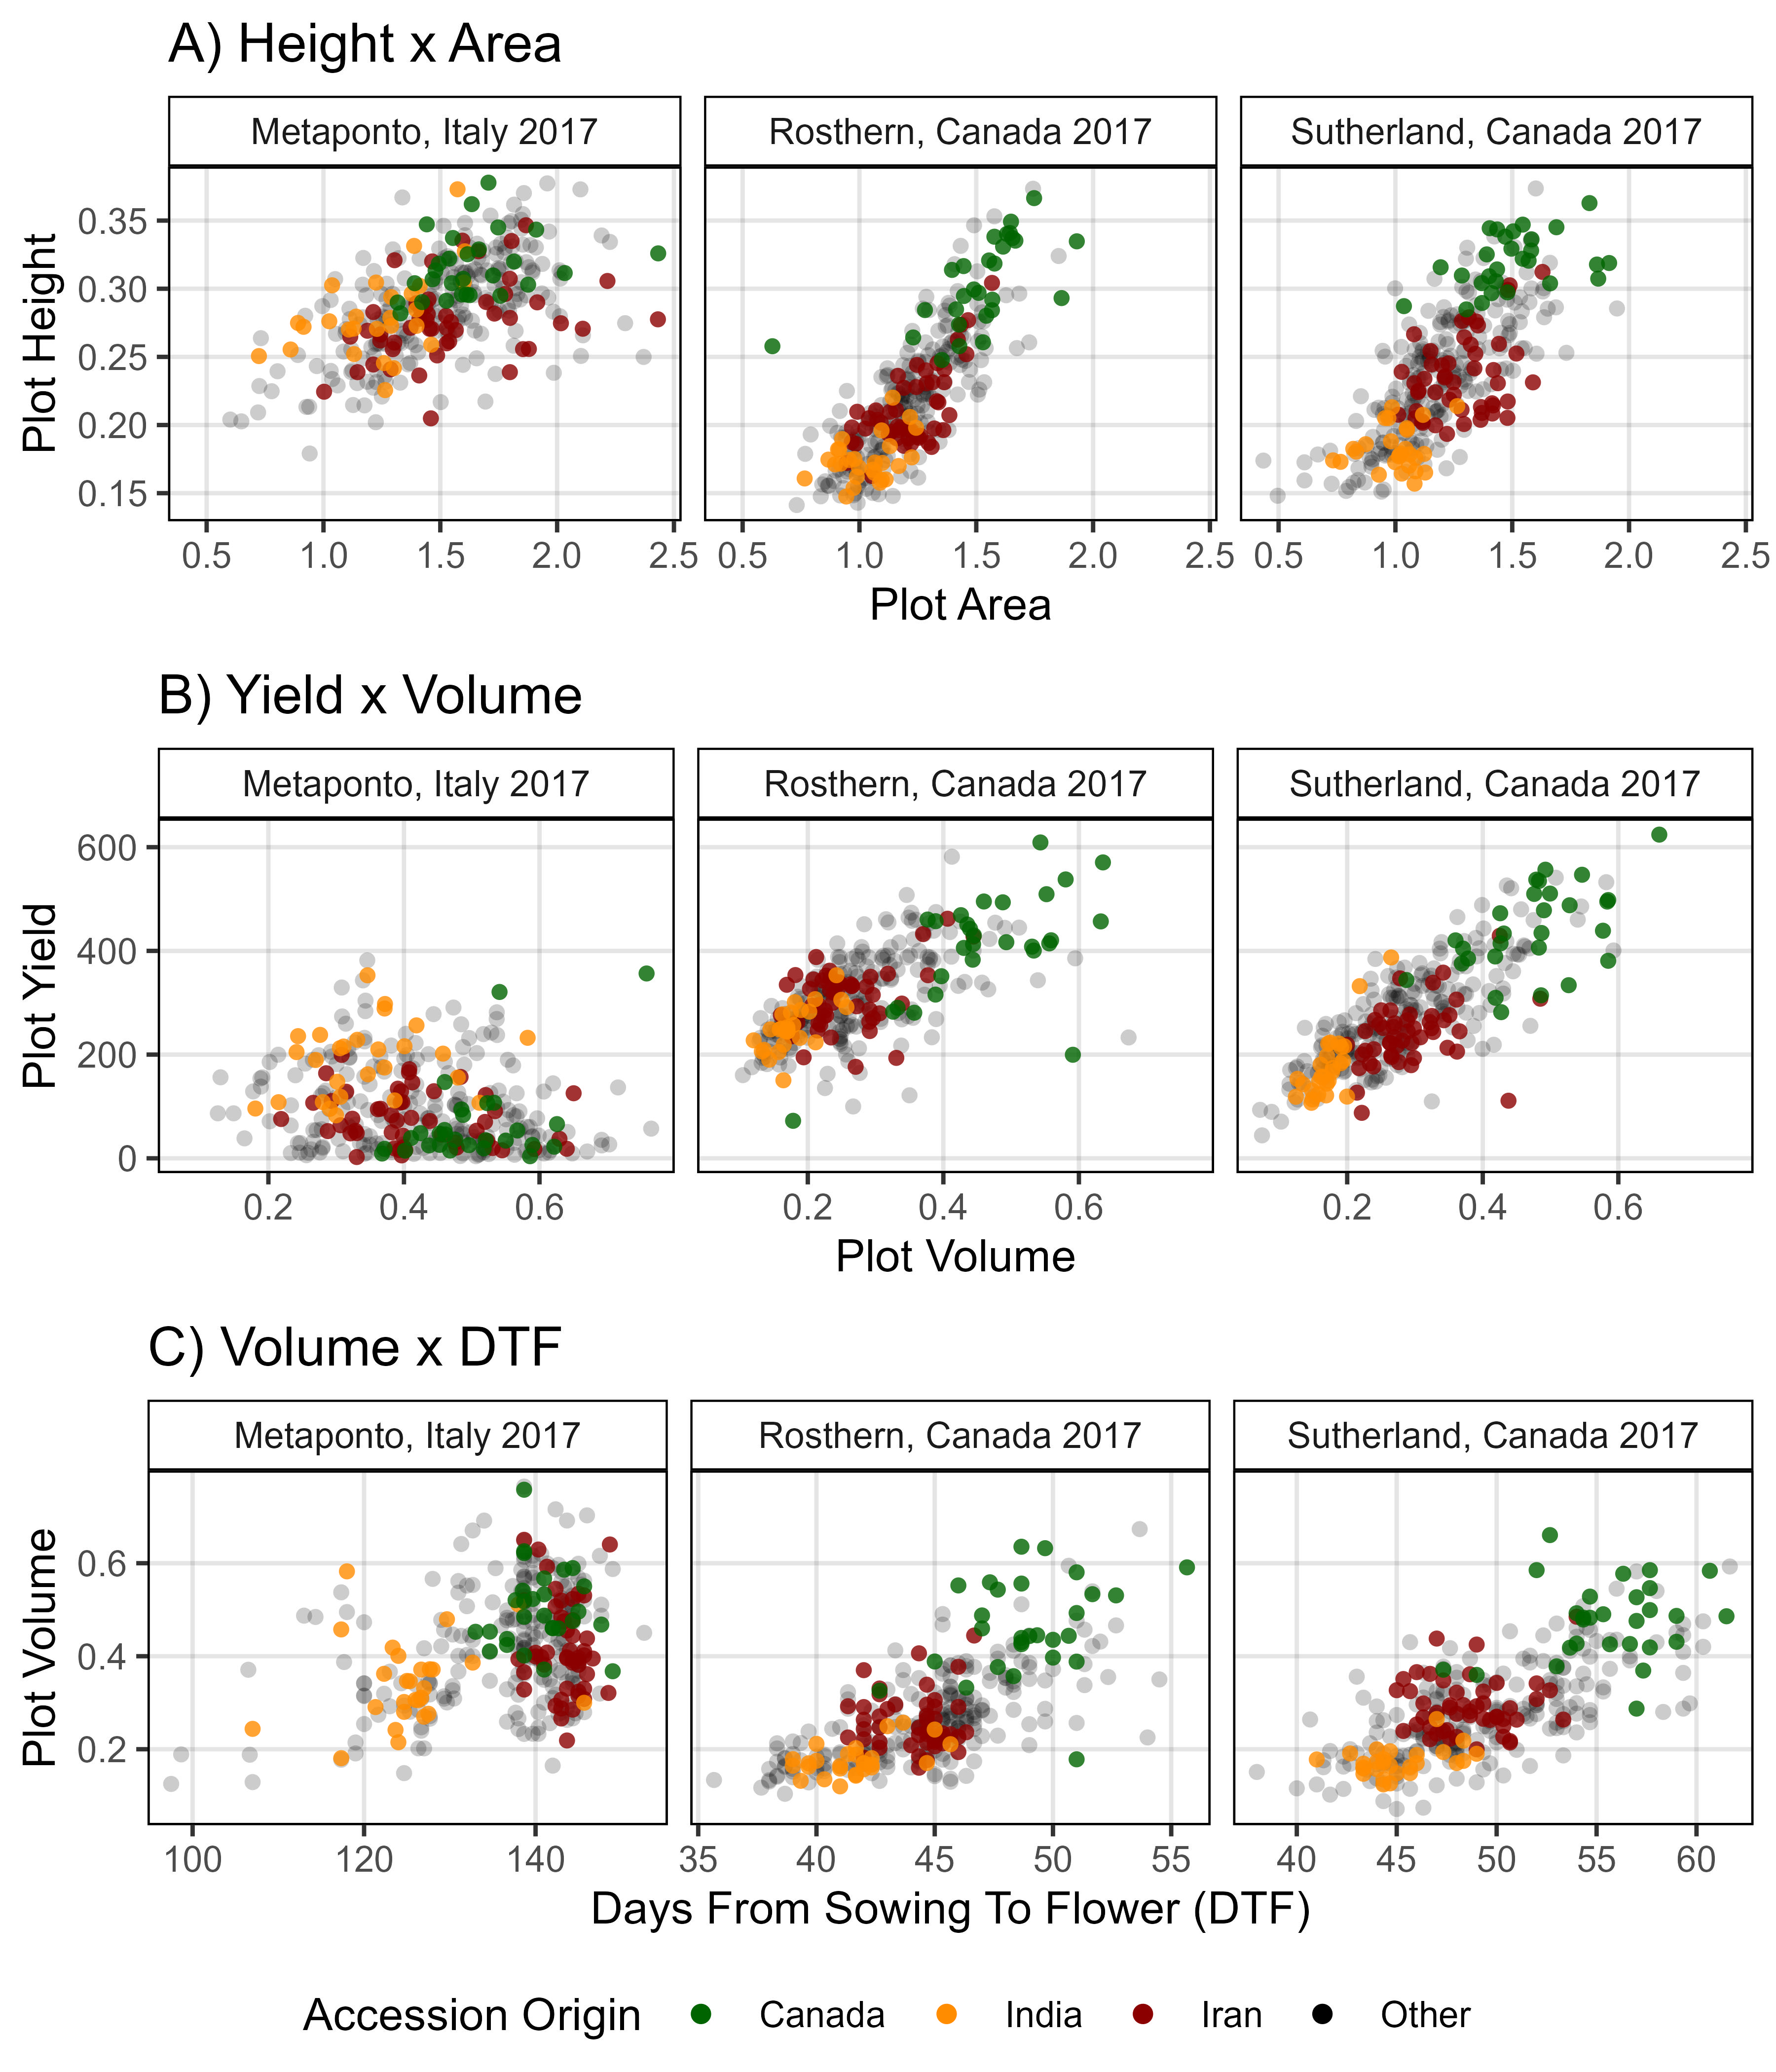
\includegraphics[keepaspectratio]{Figure_04.jpg}}

\begin{center}\rule{0.5\linewidth}{0.5pt}\end{center}

\subsection{Figure 5}\label{figure-5}

\pandocbounded{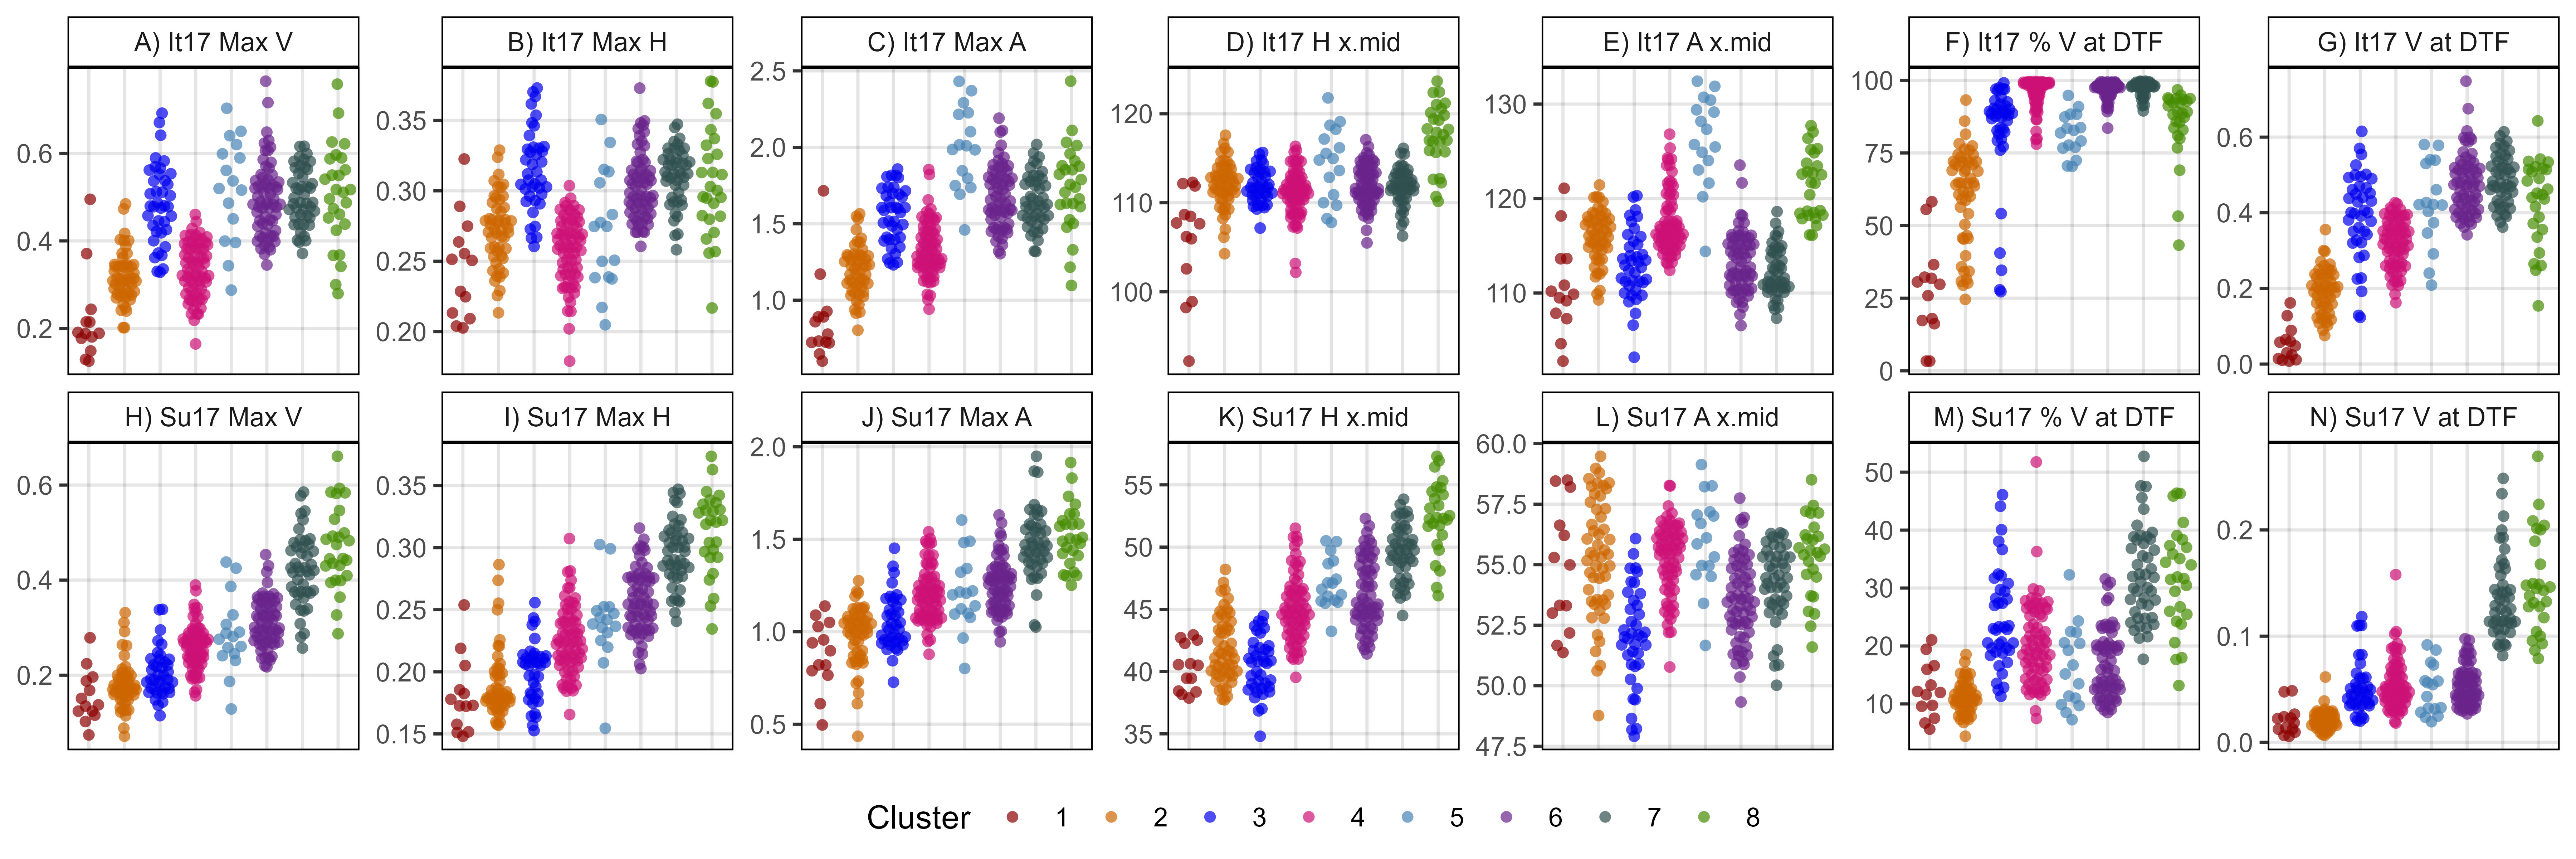
\includegraphics[keepaspectratio]{Figure_05.jpg}}

\begin{center}\rule{0.5\linewidth}{0.5pt}\end{center}

\subsection{Figure 6}\label{figure-6}

\pandocbounded{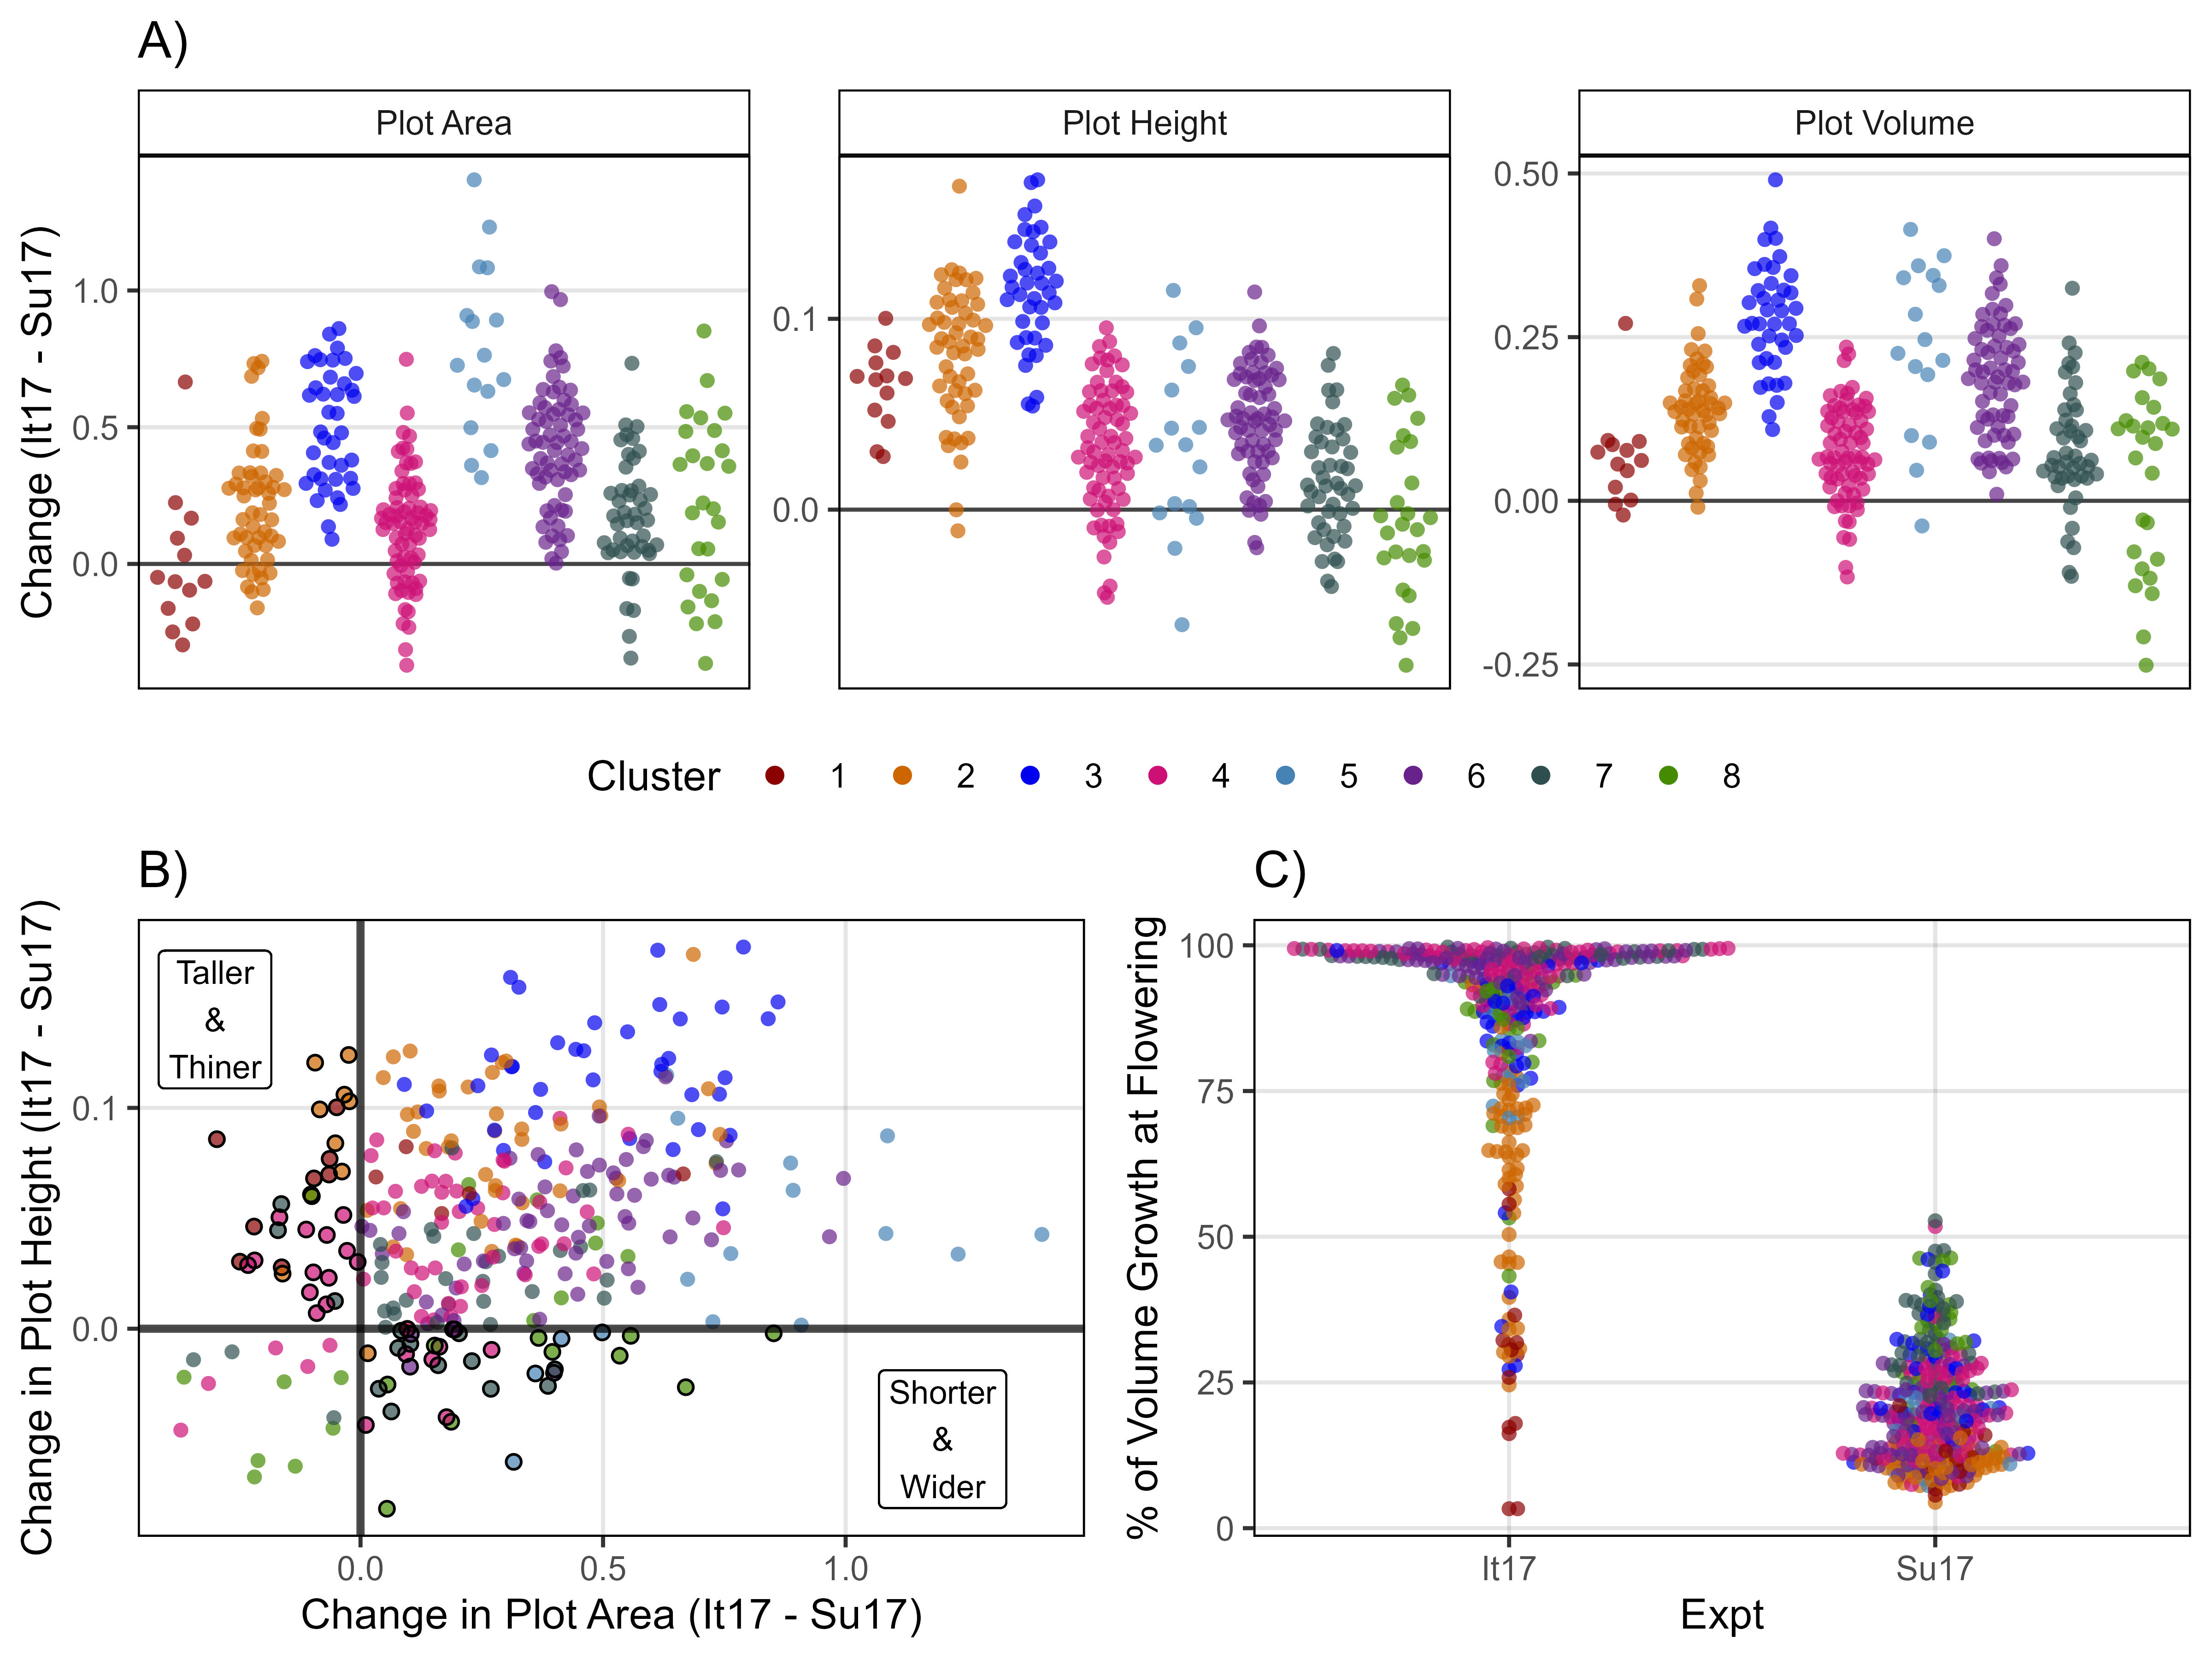
\includegraphics[keepaspectratio]{Figure_06.jpg}}

\begin{center}\rule{0.5\linewidth}{0.5pt}\end{center}

\subsection{Figure 7}\label{figure-7}

\pandocbounded{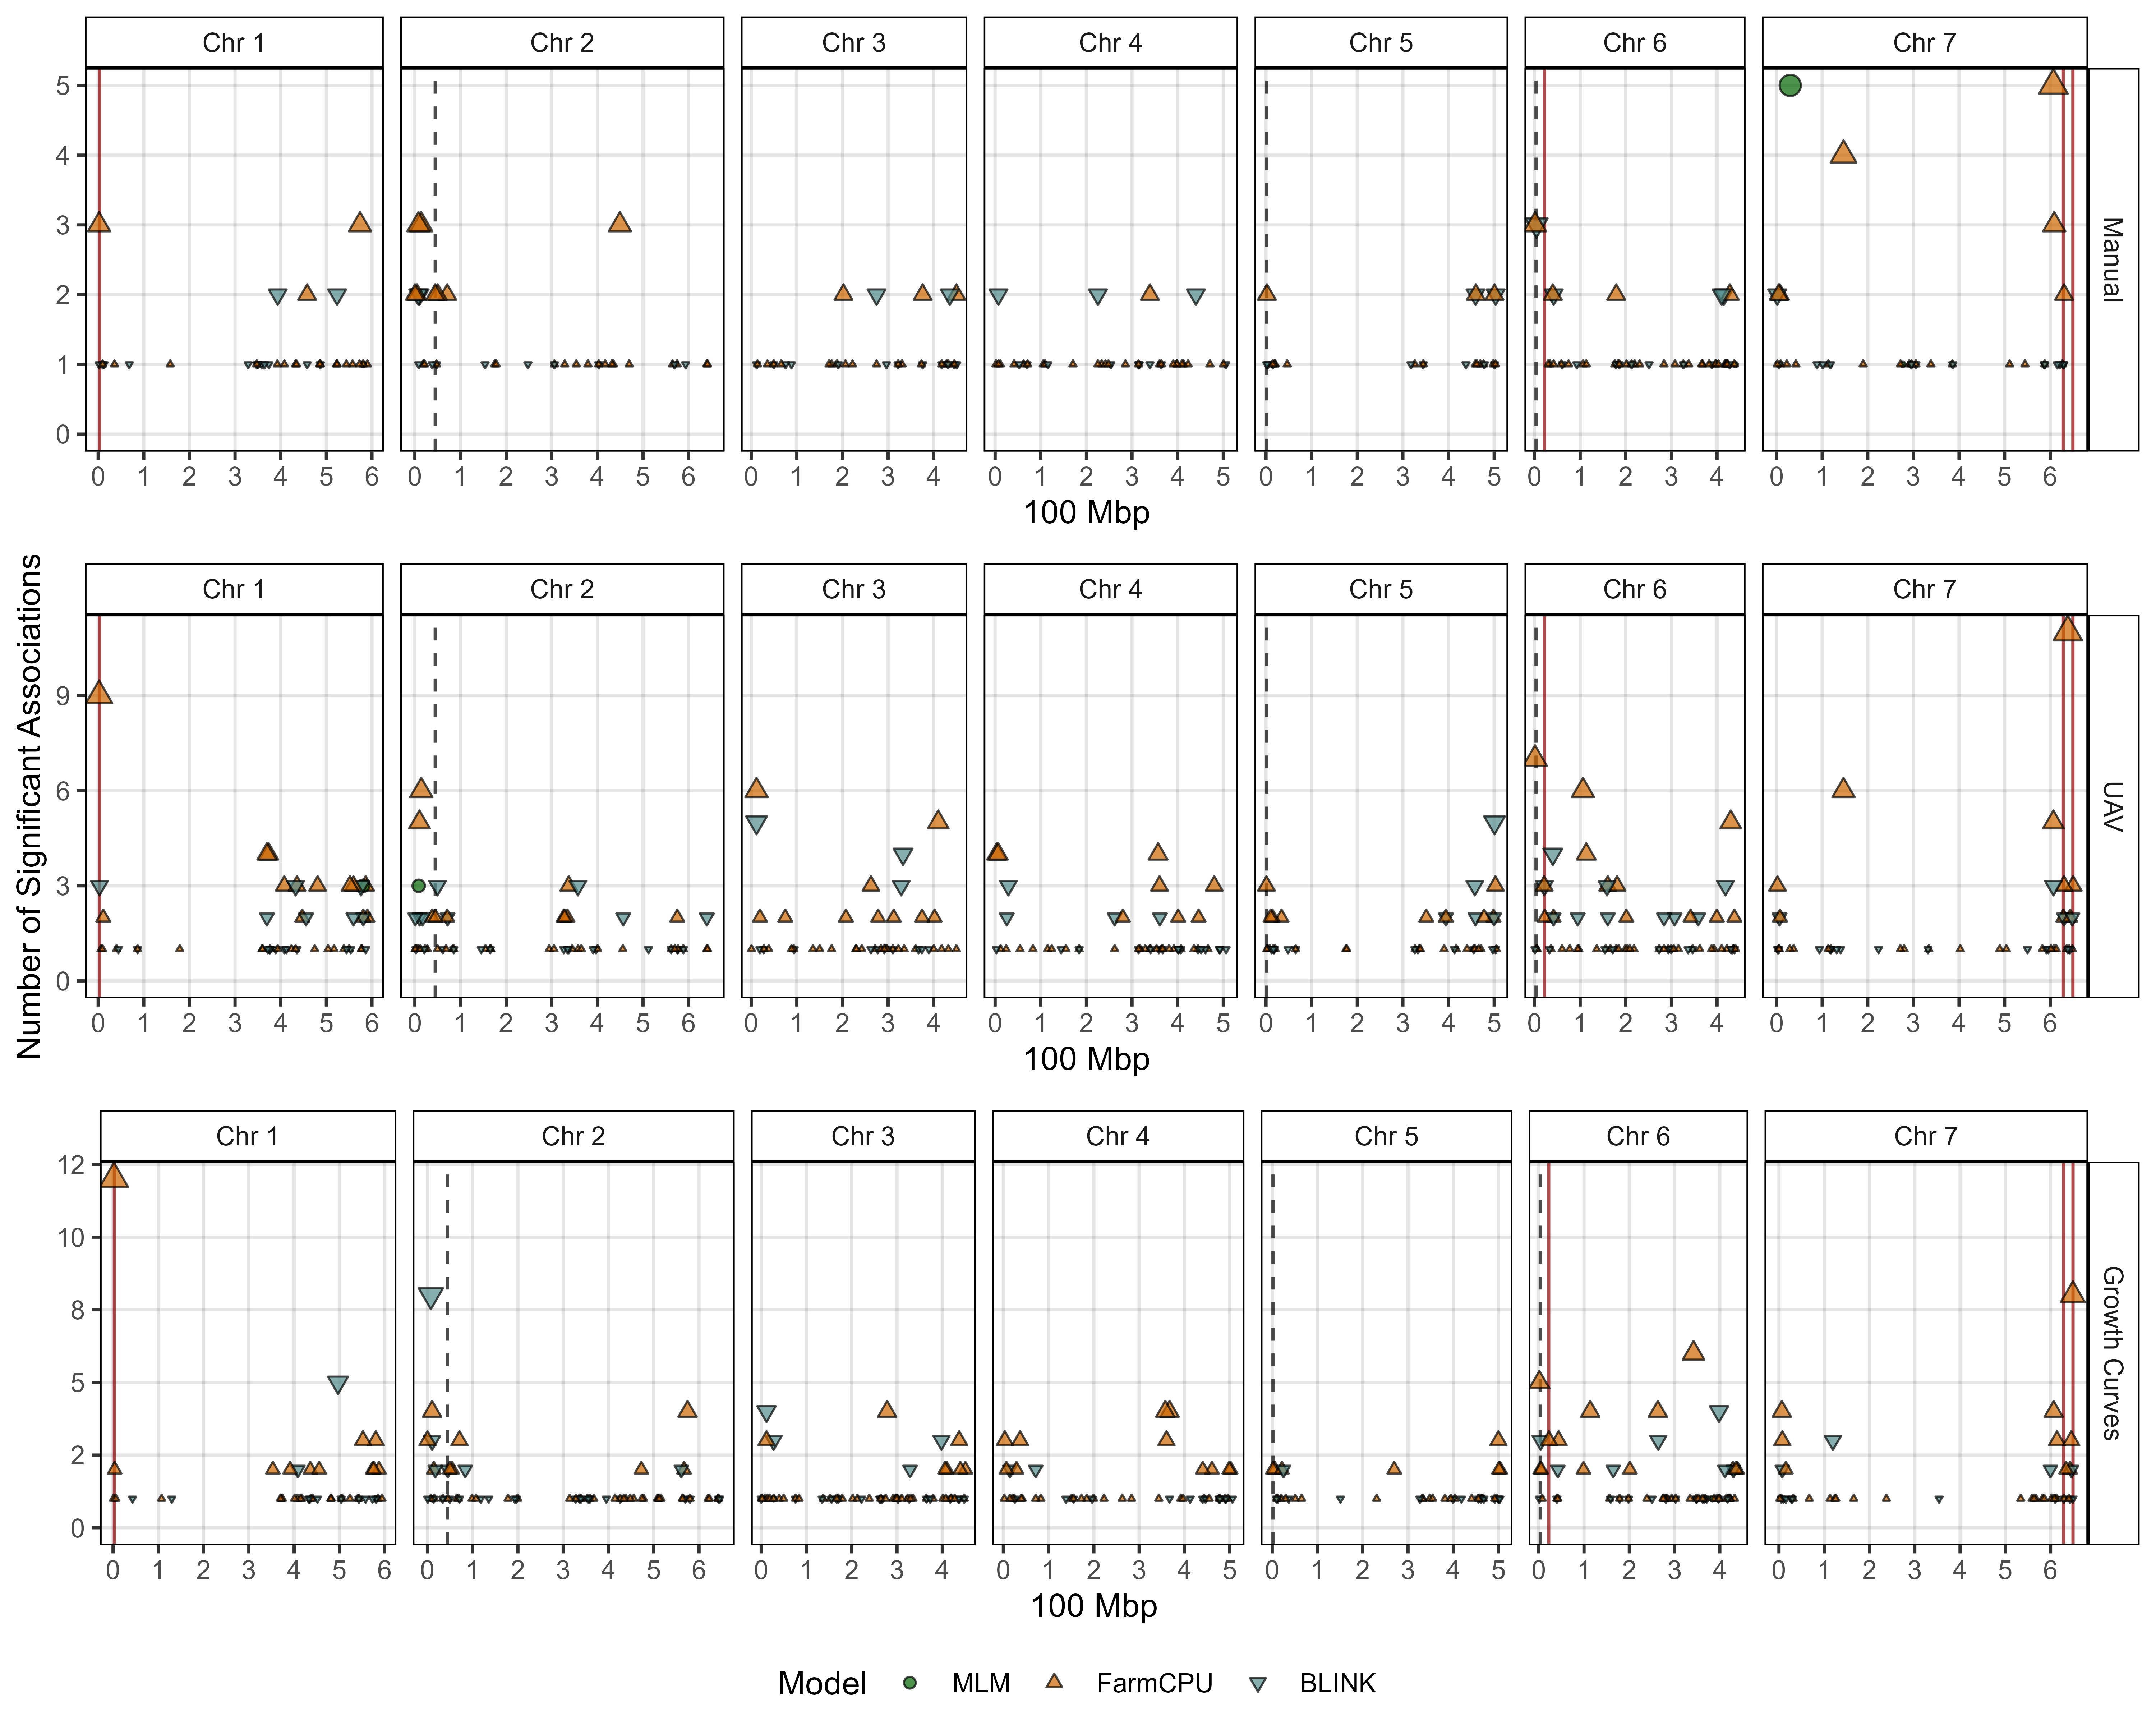
\includegraphics[keepaspectratio]{Figure_07.jpg}}

\begin{center}\rule{0.5\linewidth}{0.5pt}\end{center}

\subsection{Figure 8}\label{figure-8}

\pandocbounded{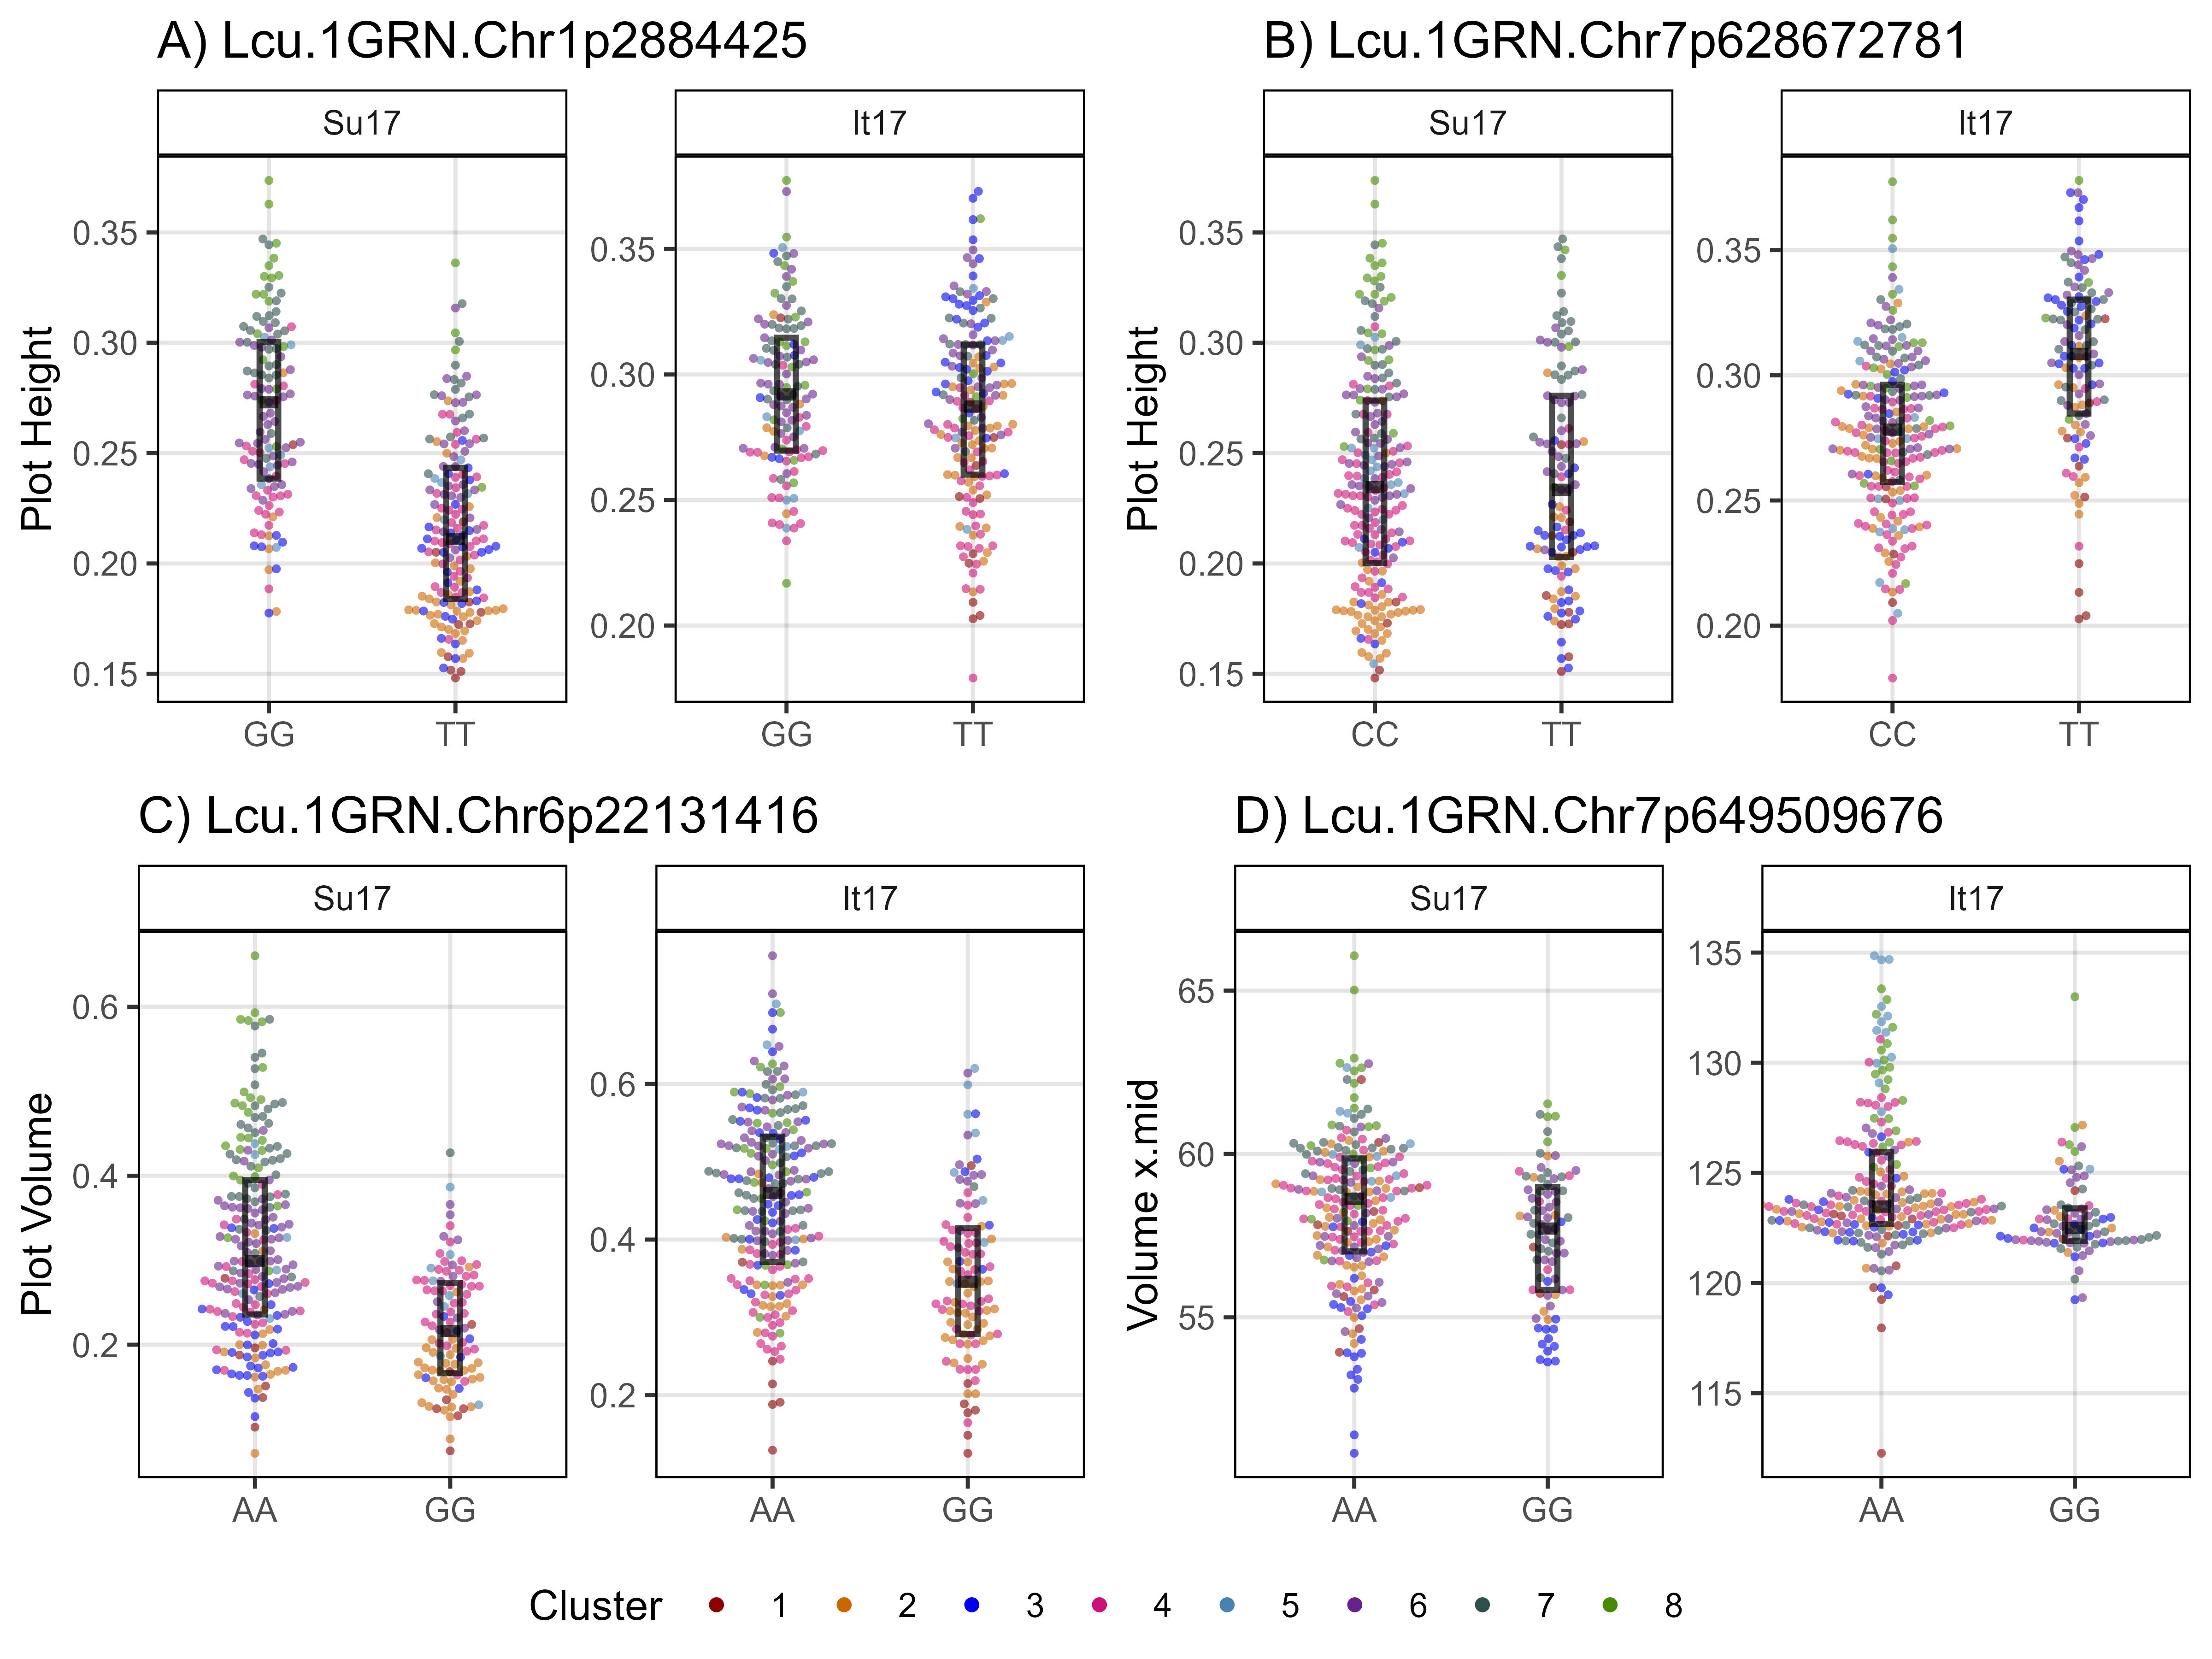
\includegraphics[keepaspectratio]{Figure_08.jpg}}

\begin{center}\rule{0.5\linewidth}{0.5pt}\end{center}

\section{Supplemental Tables}\label{supplemental-tables}

\subsection{Supplemental Table 1}\label{supplemental-table-1}

\begin{quote}
\begin{itemize}
\tightlist
\item
  \href{https://github.com/derekmichaelwright/AGILE_LDP_UAV/blob/master/Supplemental_Table_01.csv}{Supplemental\_Table\_01.csv}
\end{itemize}
\end{quote}

\begin{center}\rule{0.5\linewidth}{0.5pt}\end{center}

\section{Supplemental Figures}\label{supplemental-figures}

\subsection{Supplemental Figure 1}\label{supplemental-figure-1}

\includegraphics[width=0.8\linewidth,height=\textheight,keepaspectratio]{Supplemental_Figure_01.jpg}

\begin{center}\rule{0.5\linewidth}{0.5pt}\end{center}

\subsection{Supplemental Figure 2}\label{supplemental-figure-2}

\pandocbounded{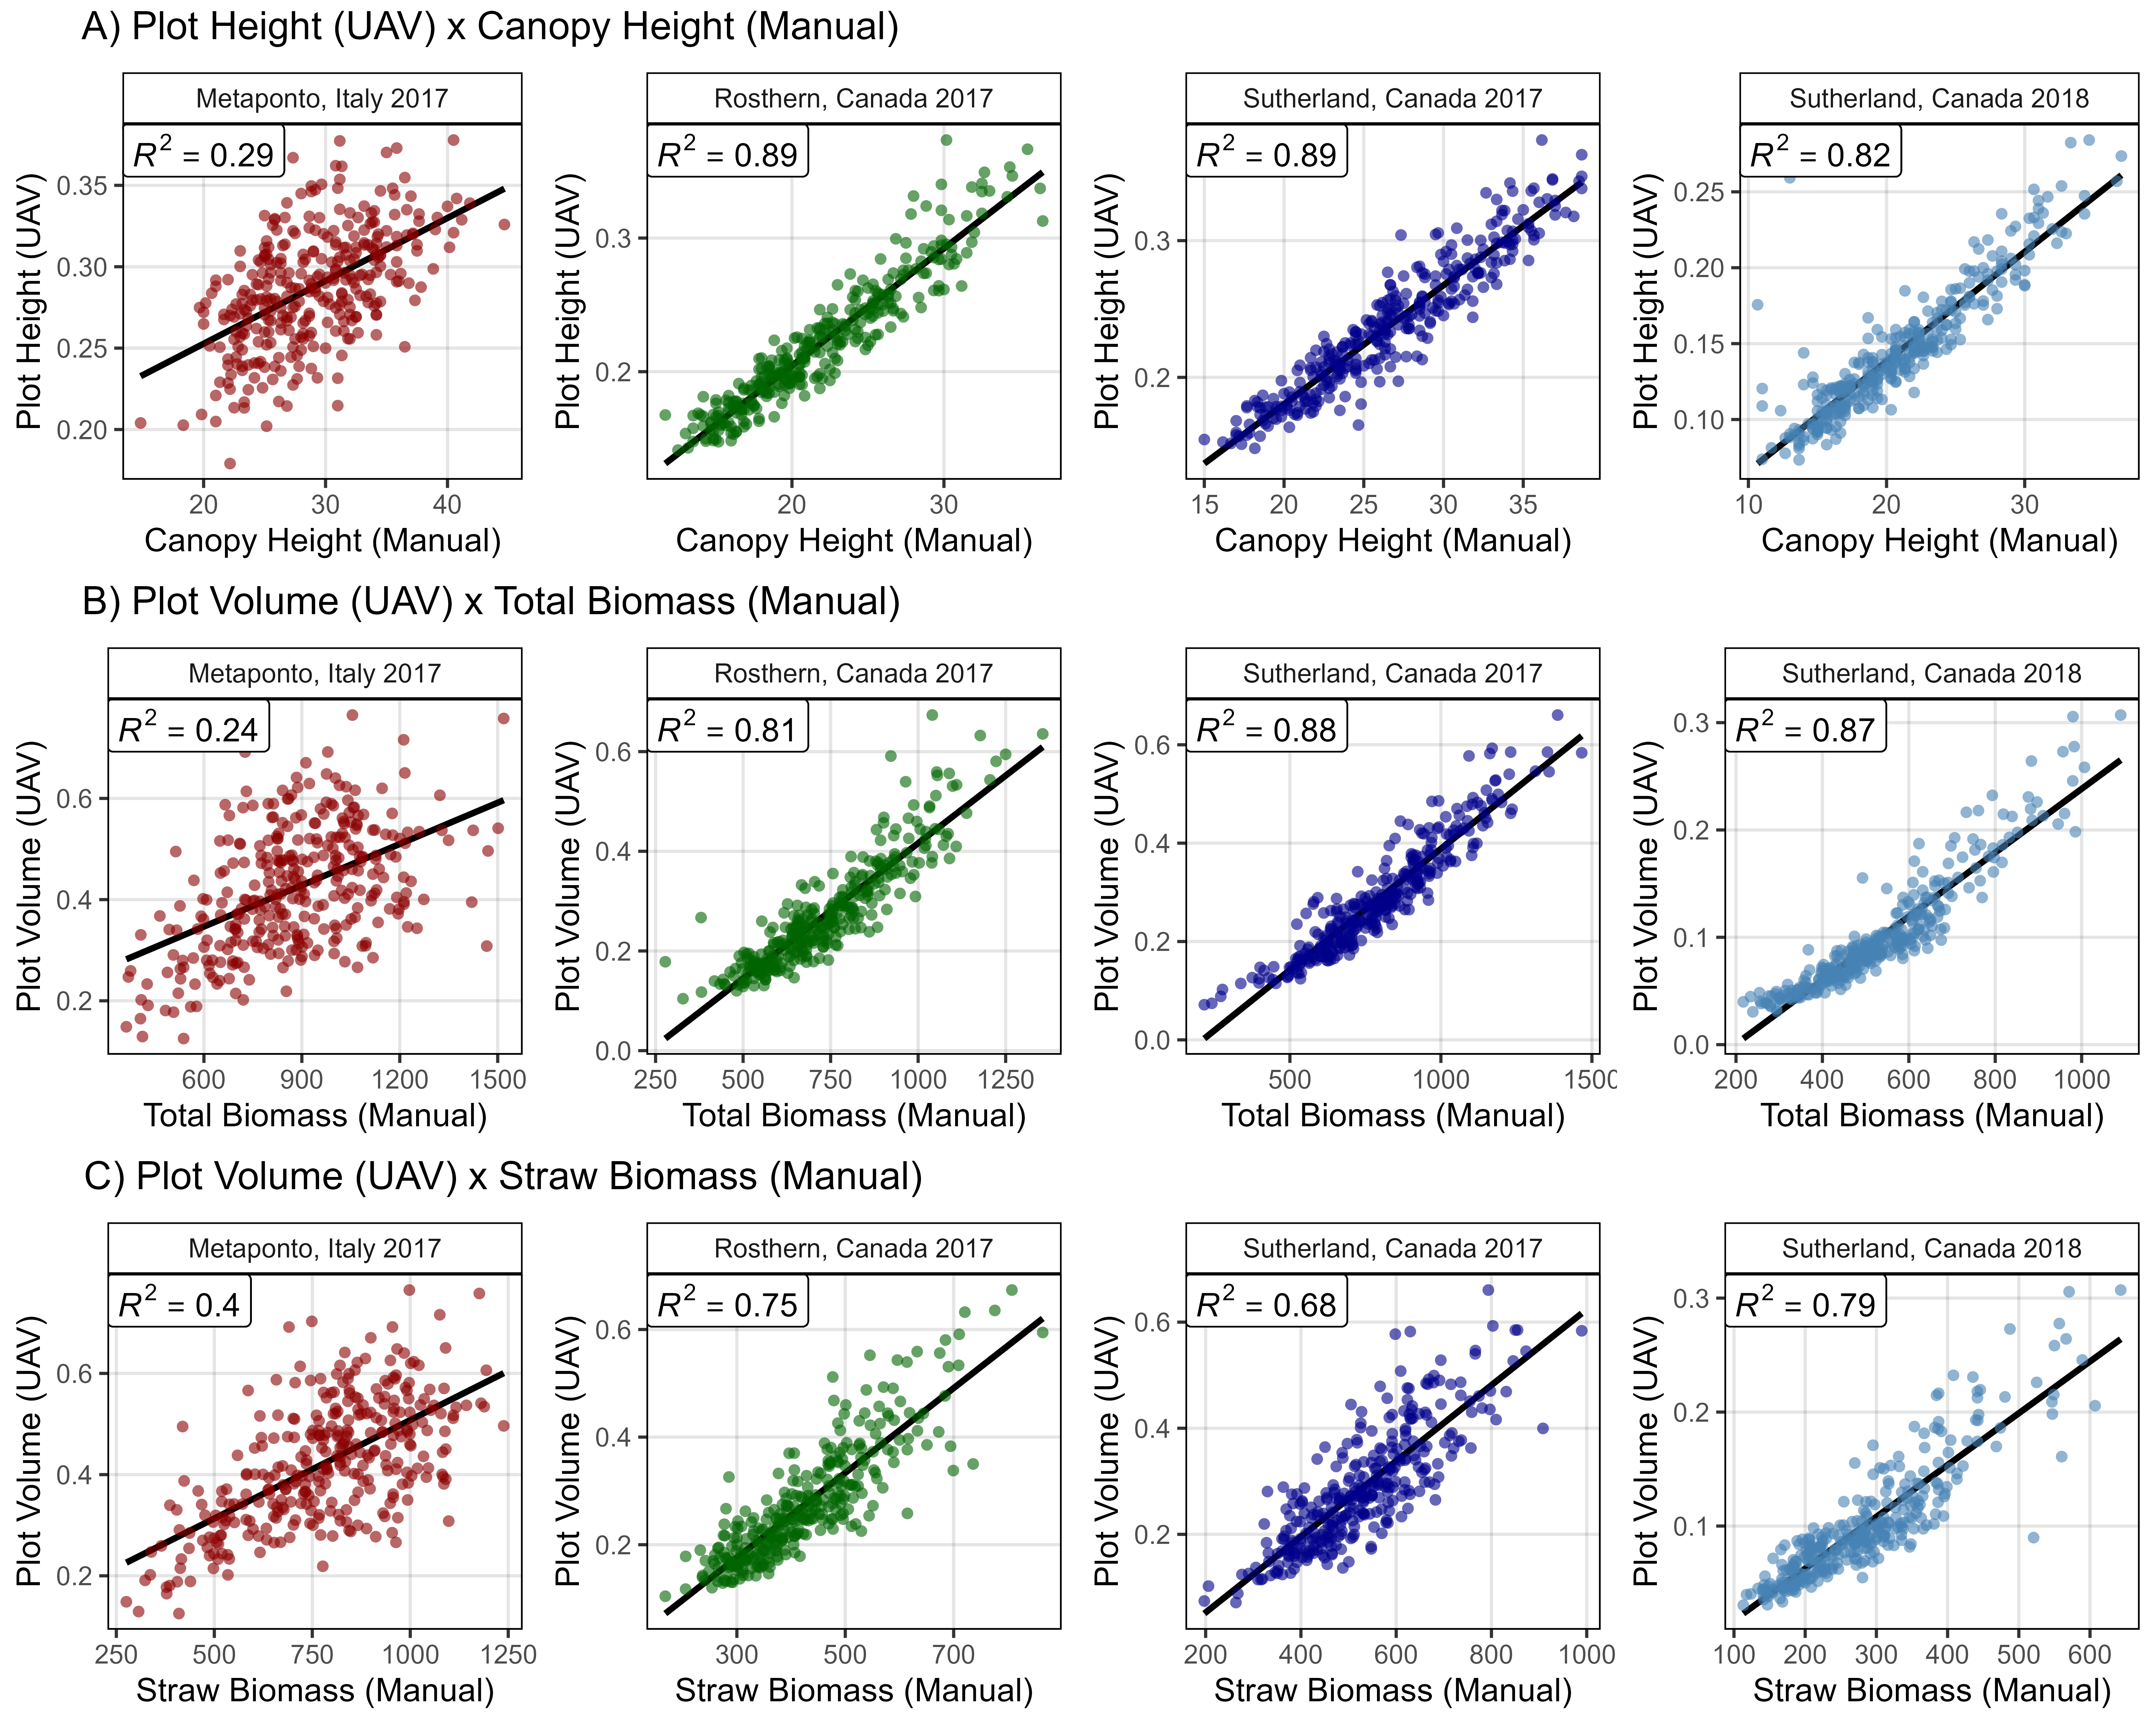
\includegraphics[keepaspectratio]{Supplemental_Figure_02.jpg}}

\begin{center}\rule{0.5\linewidth}{0.5pt}\end{center}

\subsection{Supplemental Figure 3}\label{supplemental-figure-3}

\pandocbounded{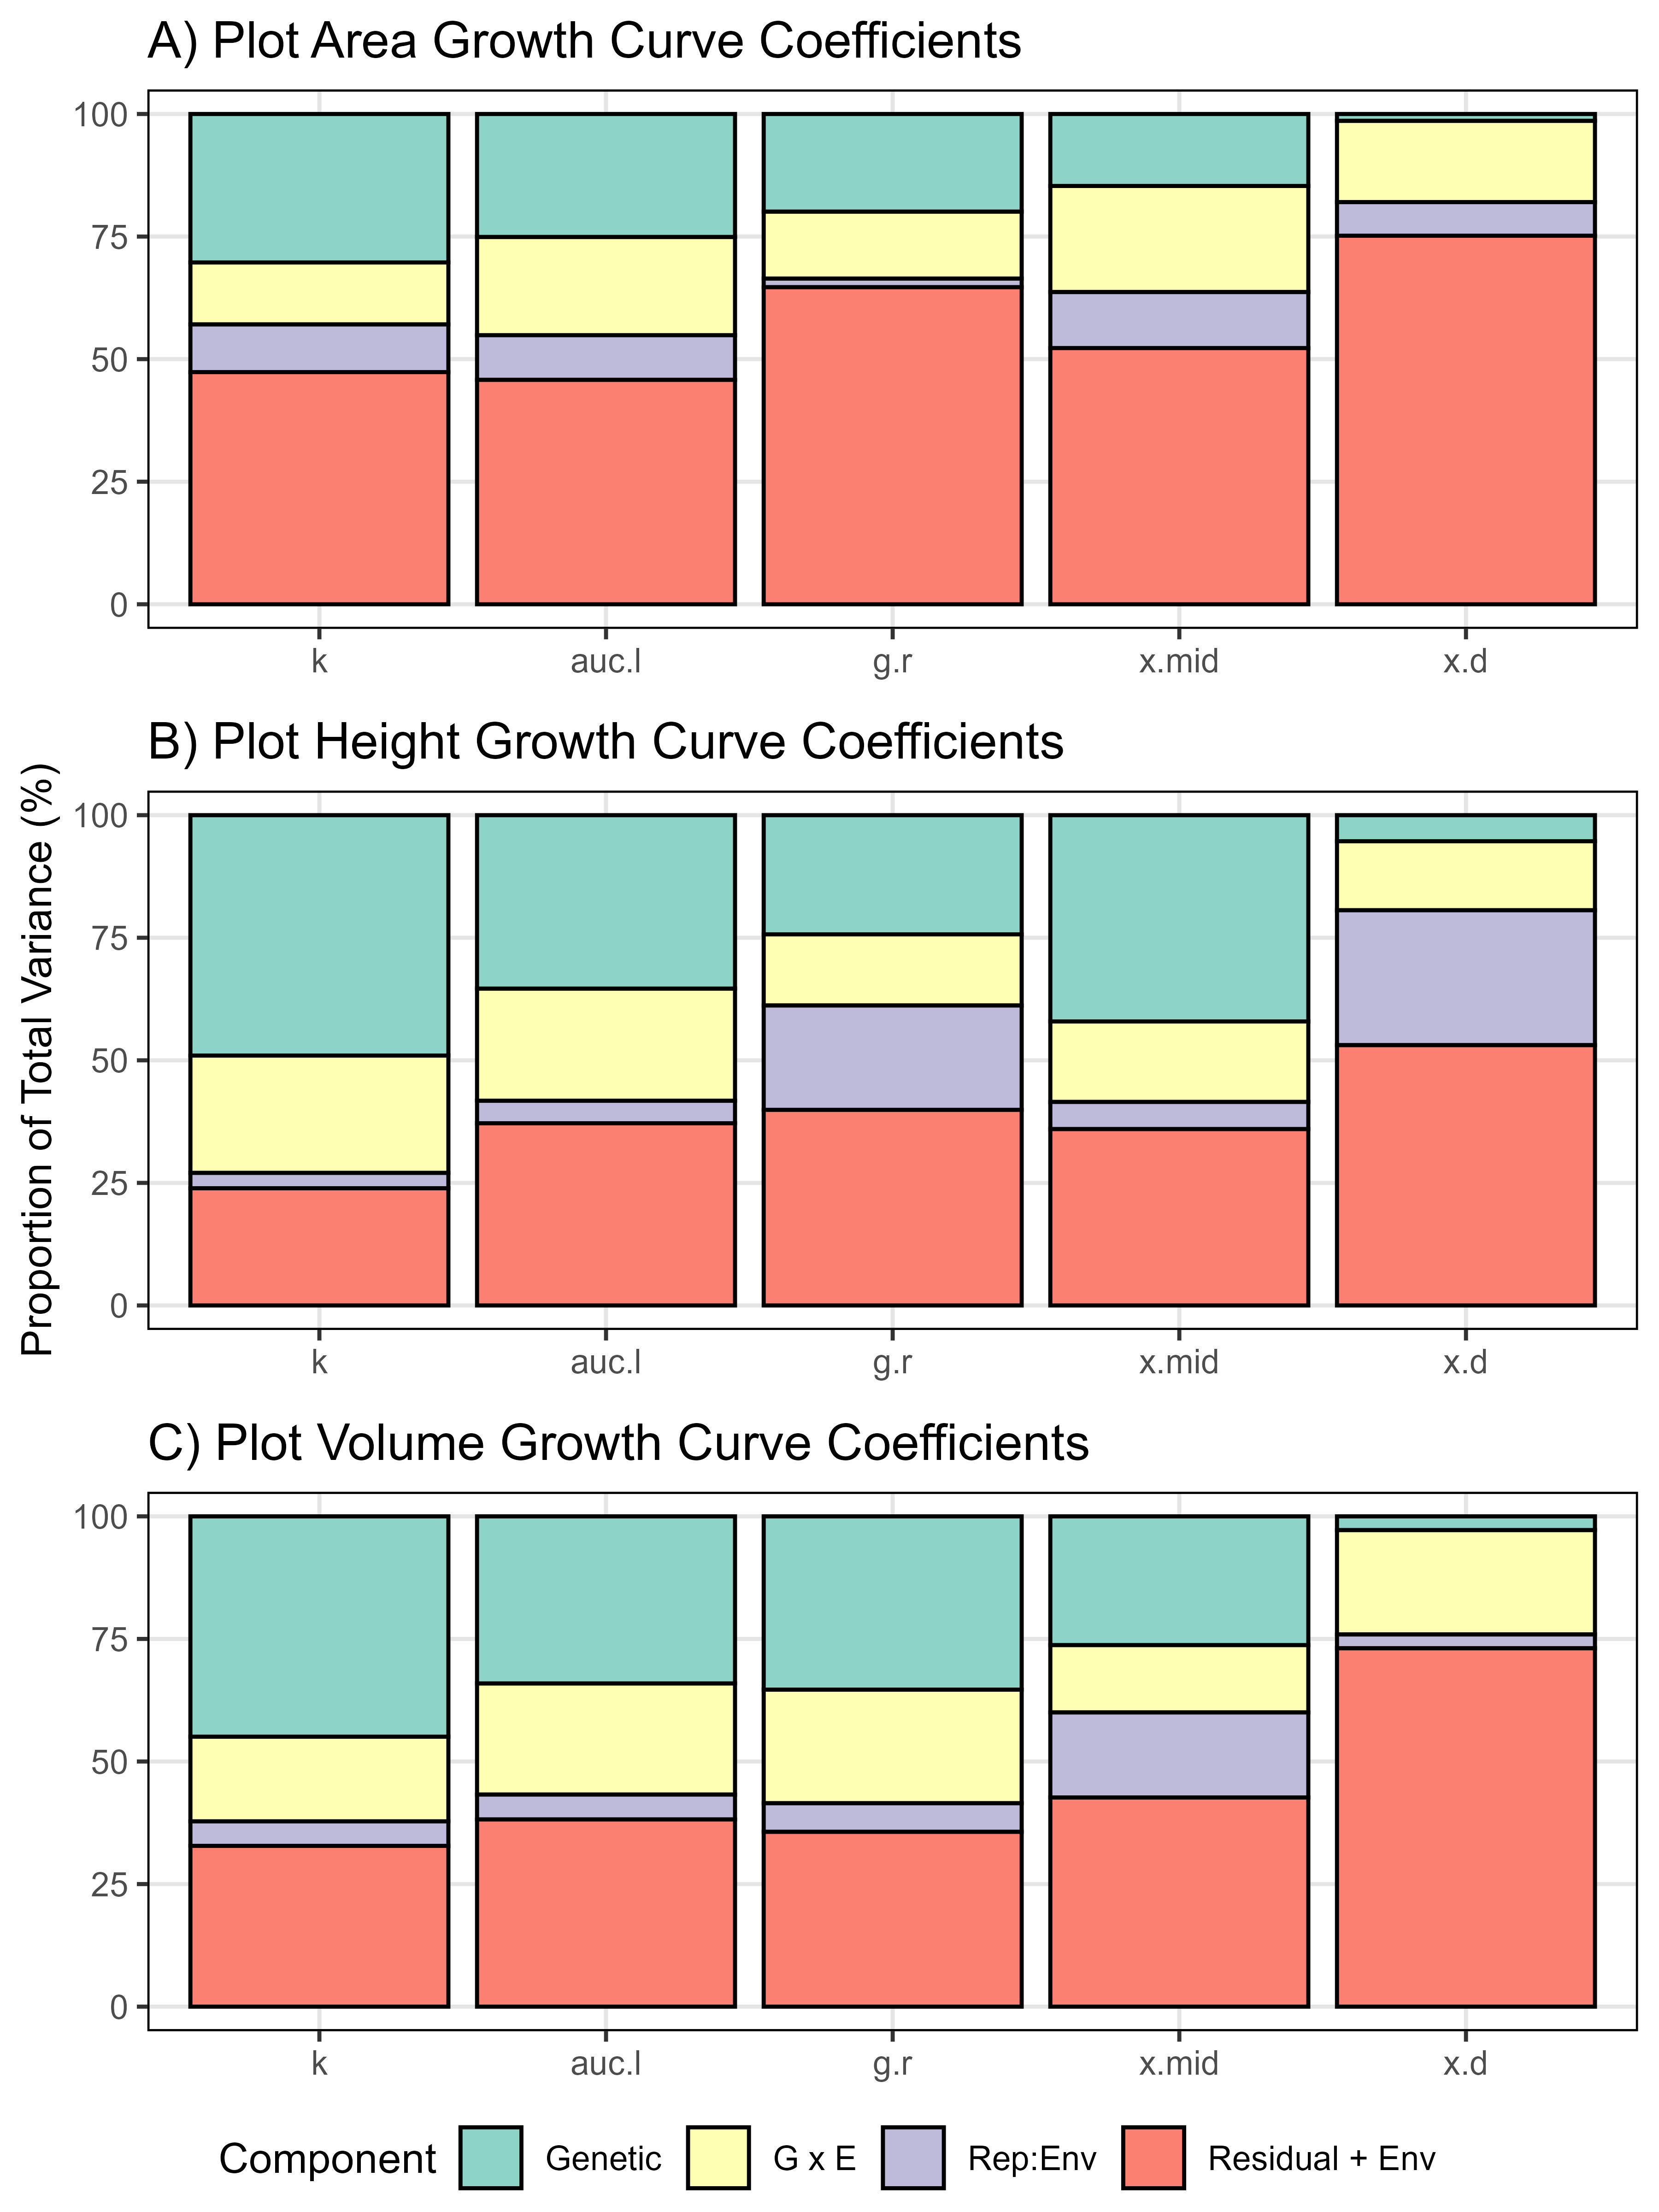
\includegraphics[keepaspectratio]{Supplemental_Figure_03.jpg}}

\begin{center}\rule{0.5\linewidth}{0.5pt}\end{center}

\subsection{Supplemental Figure 4}\label{supplemental-figure-4}

\pandocbounded{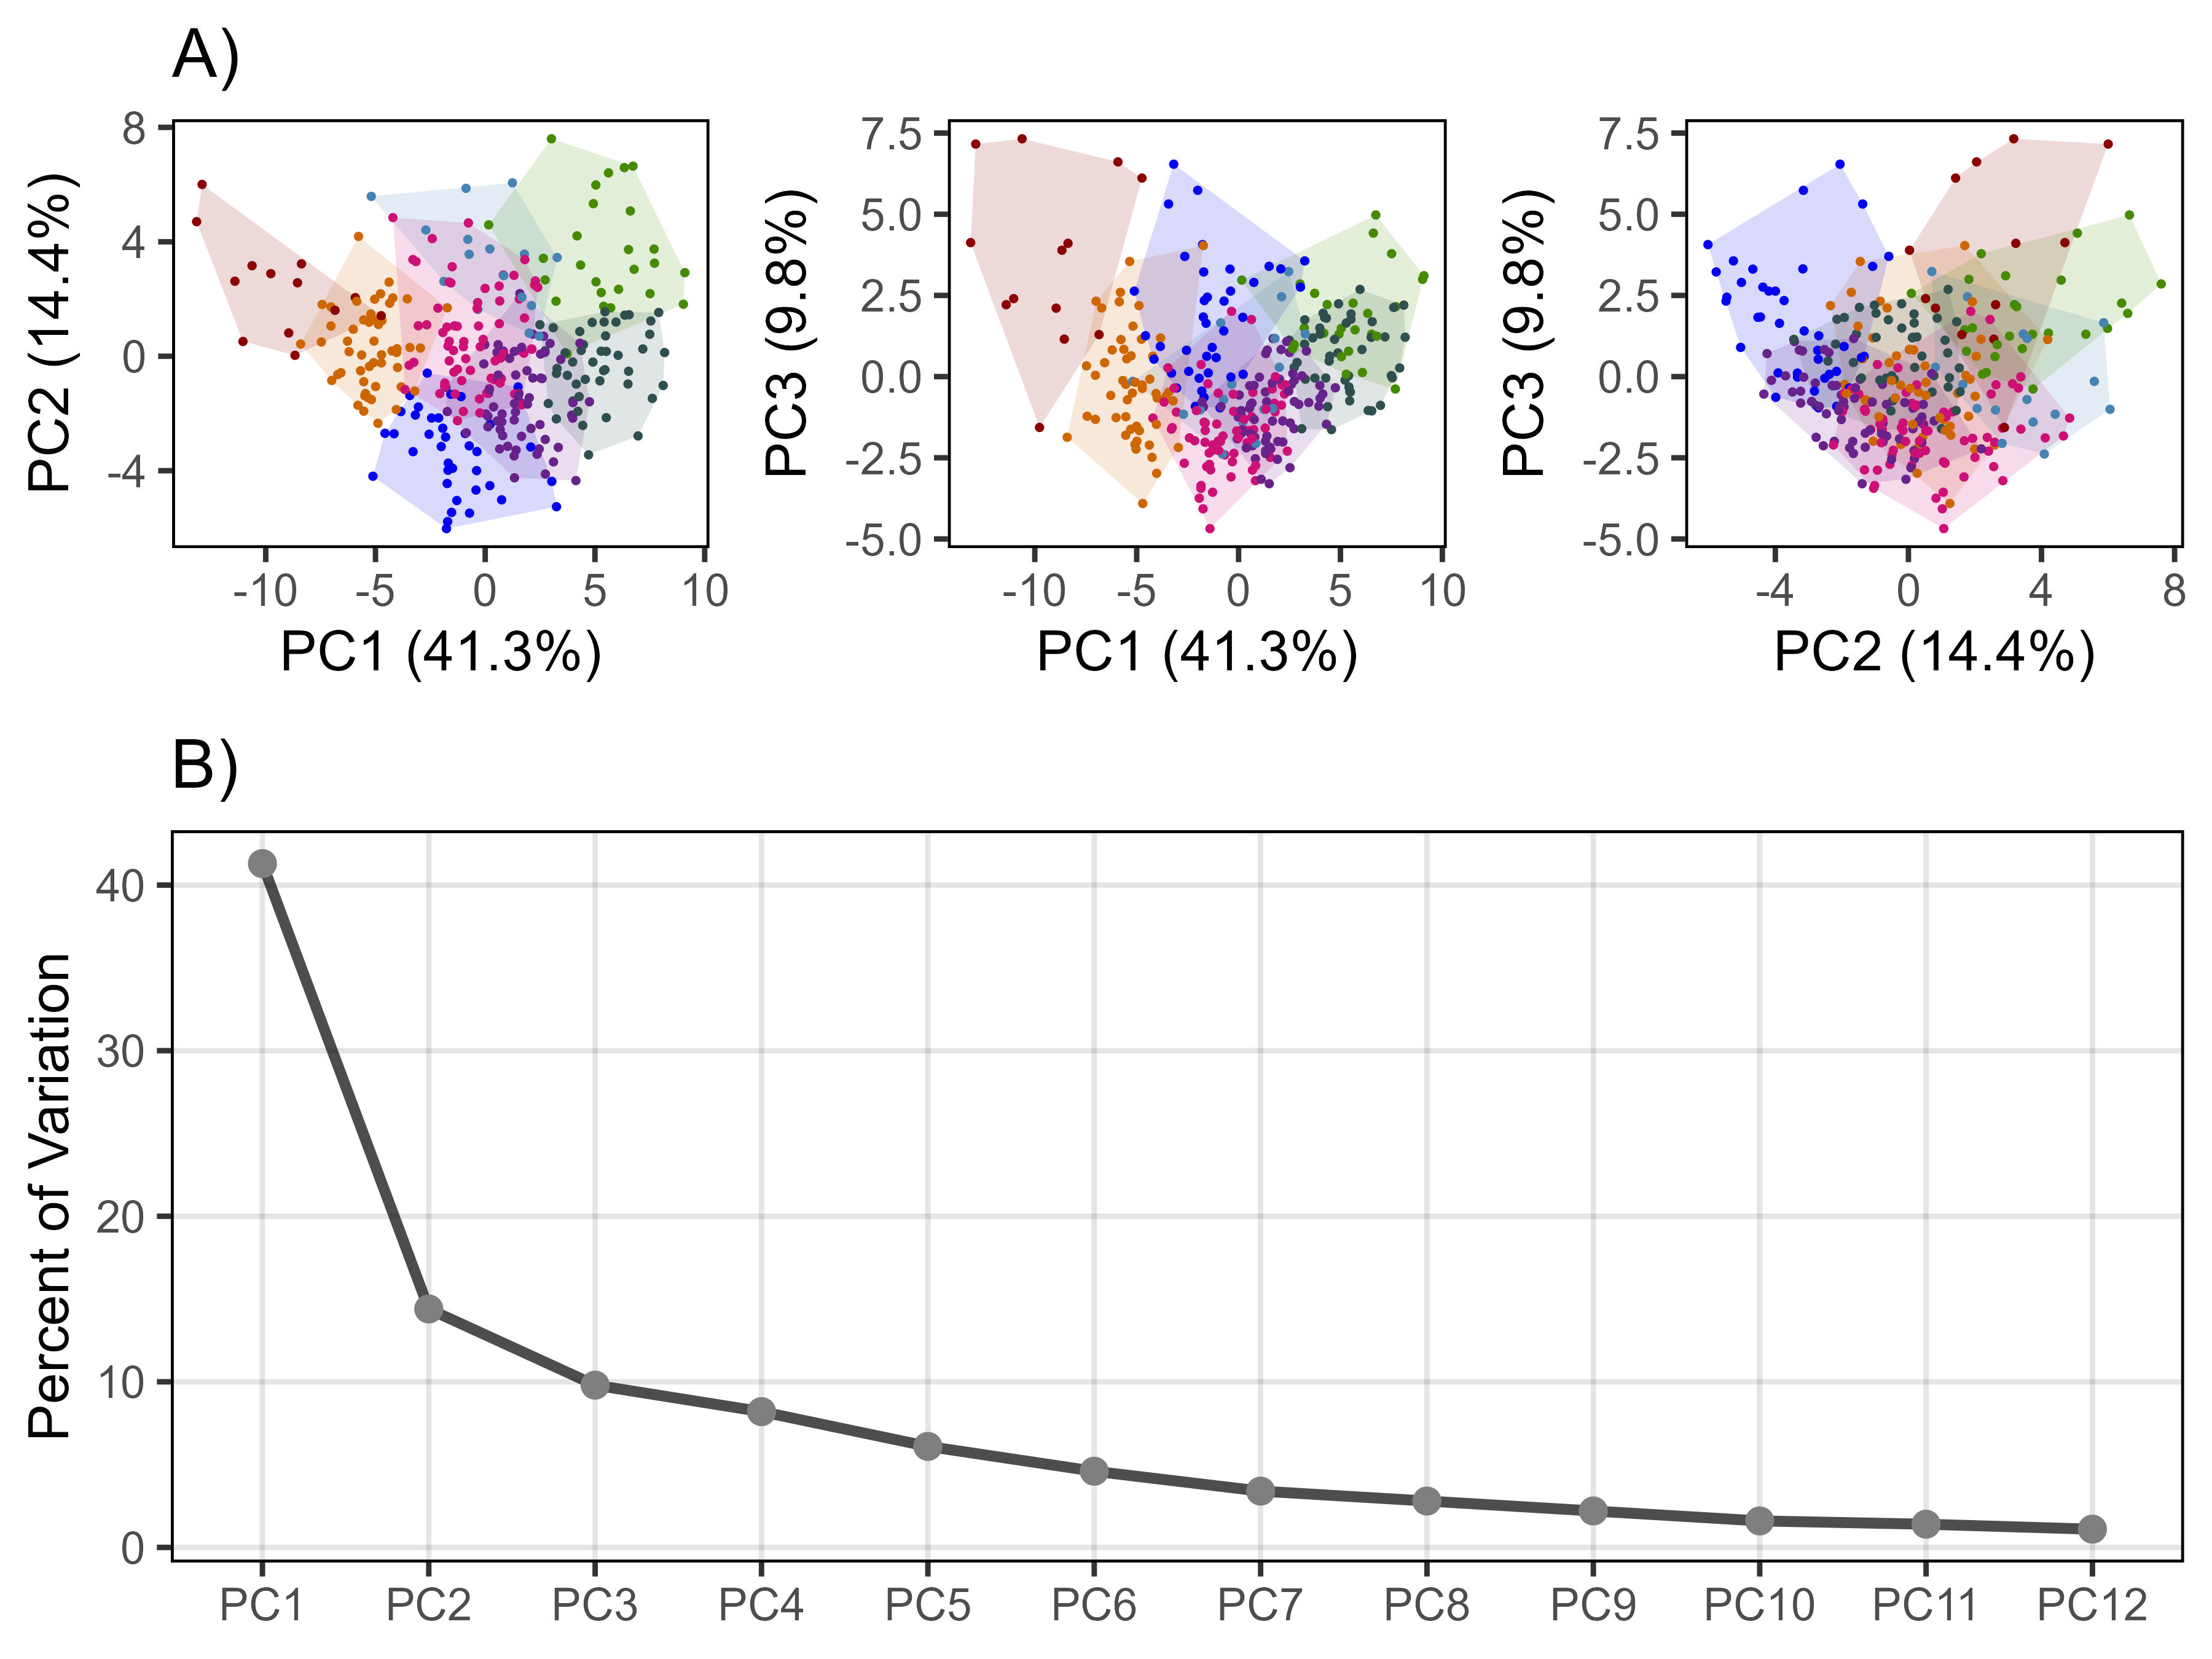
\includegraphics[keepaspectratio]{Supplemental_Figure_04.jpg}}

\begin{center}\rule{0.5\linewidth}{0.5pt}\end{center}

\subsection{Supplemental Figure 5}\label{supplemental-figure-5}

\pandocbounded{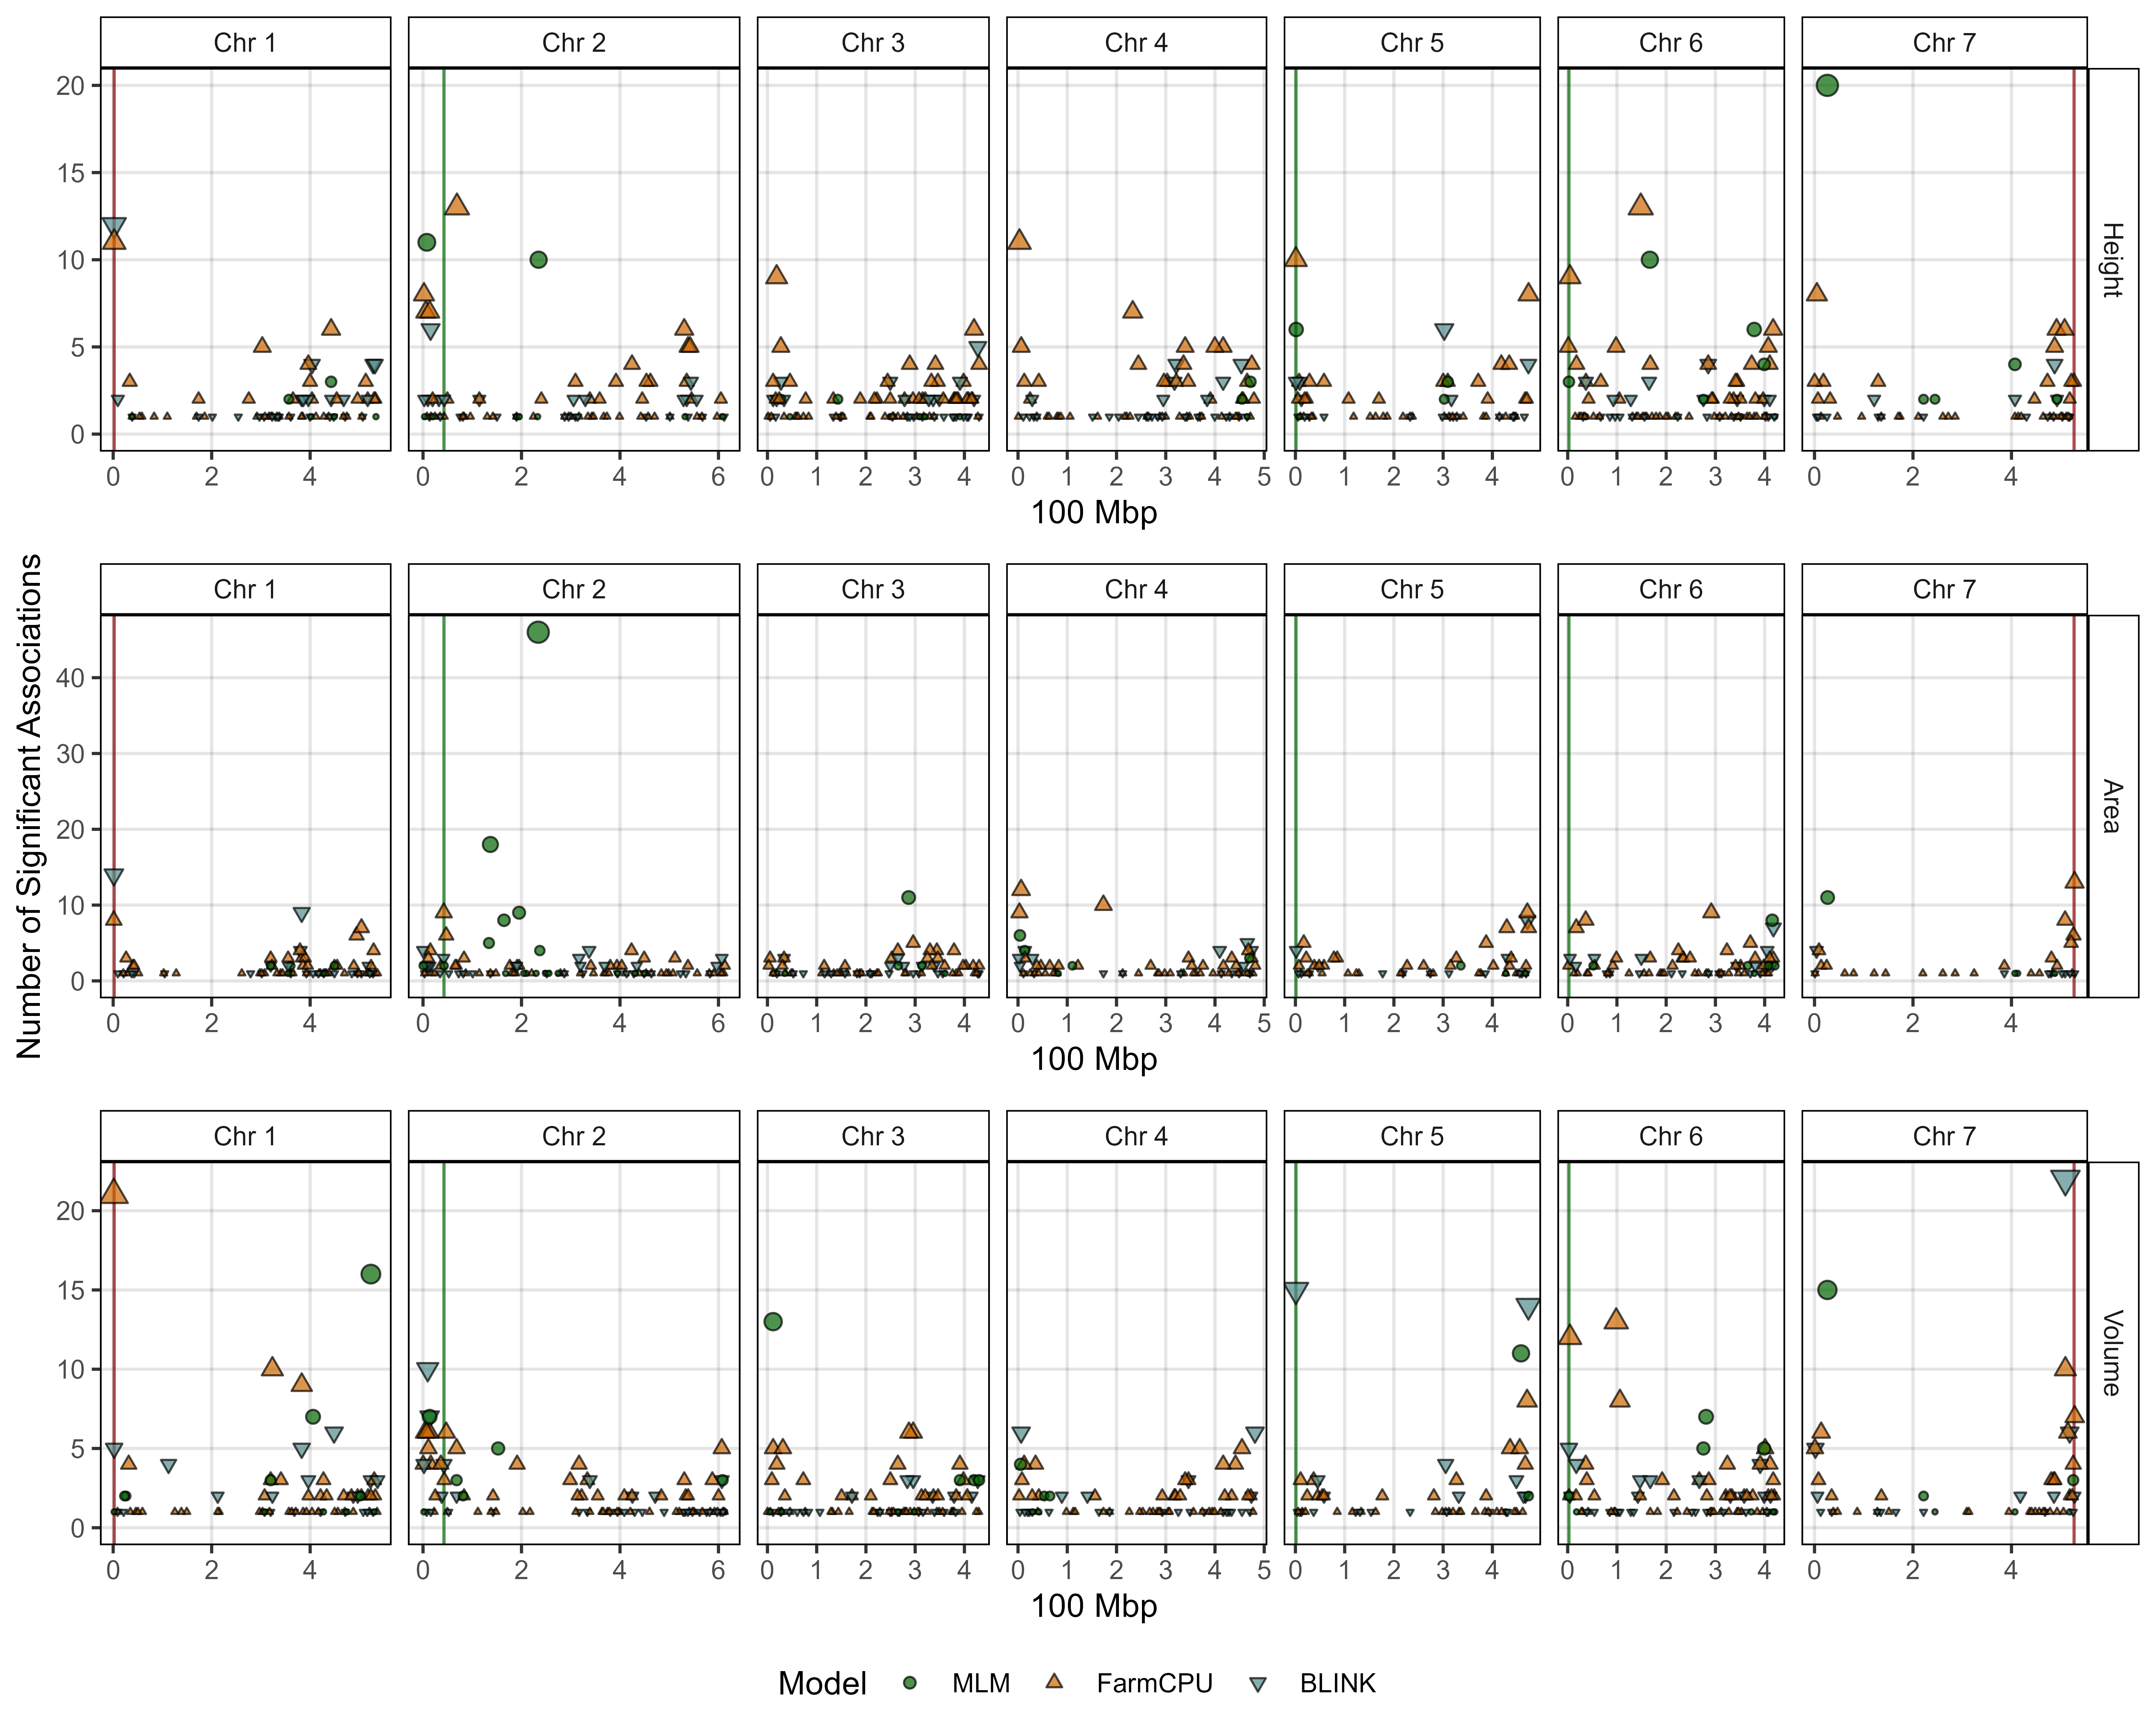
\includegraphics[keepaspectratio]{Supplemental_Figure_05.jpg}}

\begin{center}\rule{0.5\linewidth}{0.5pt}\end{center}

\subsection{Supplemental Figure 6}\label{supplemental-figure-6}

\pandocbounded{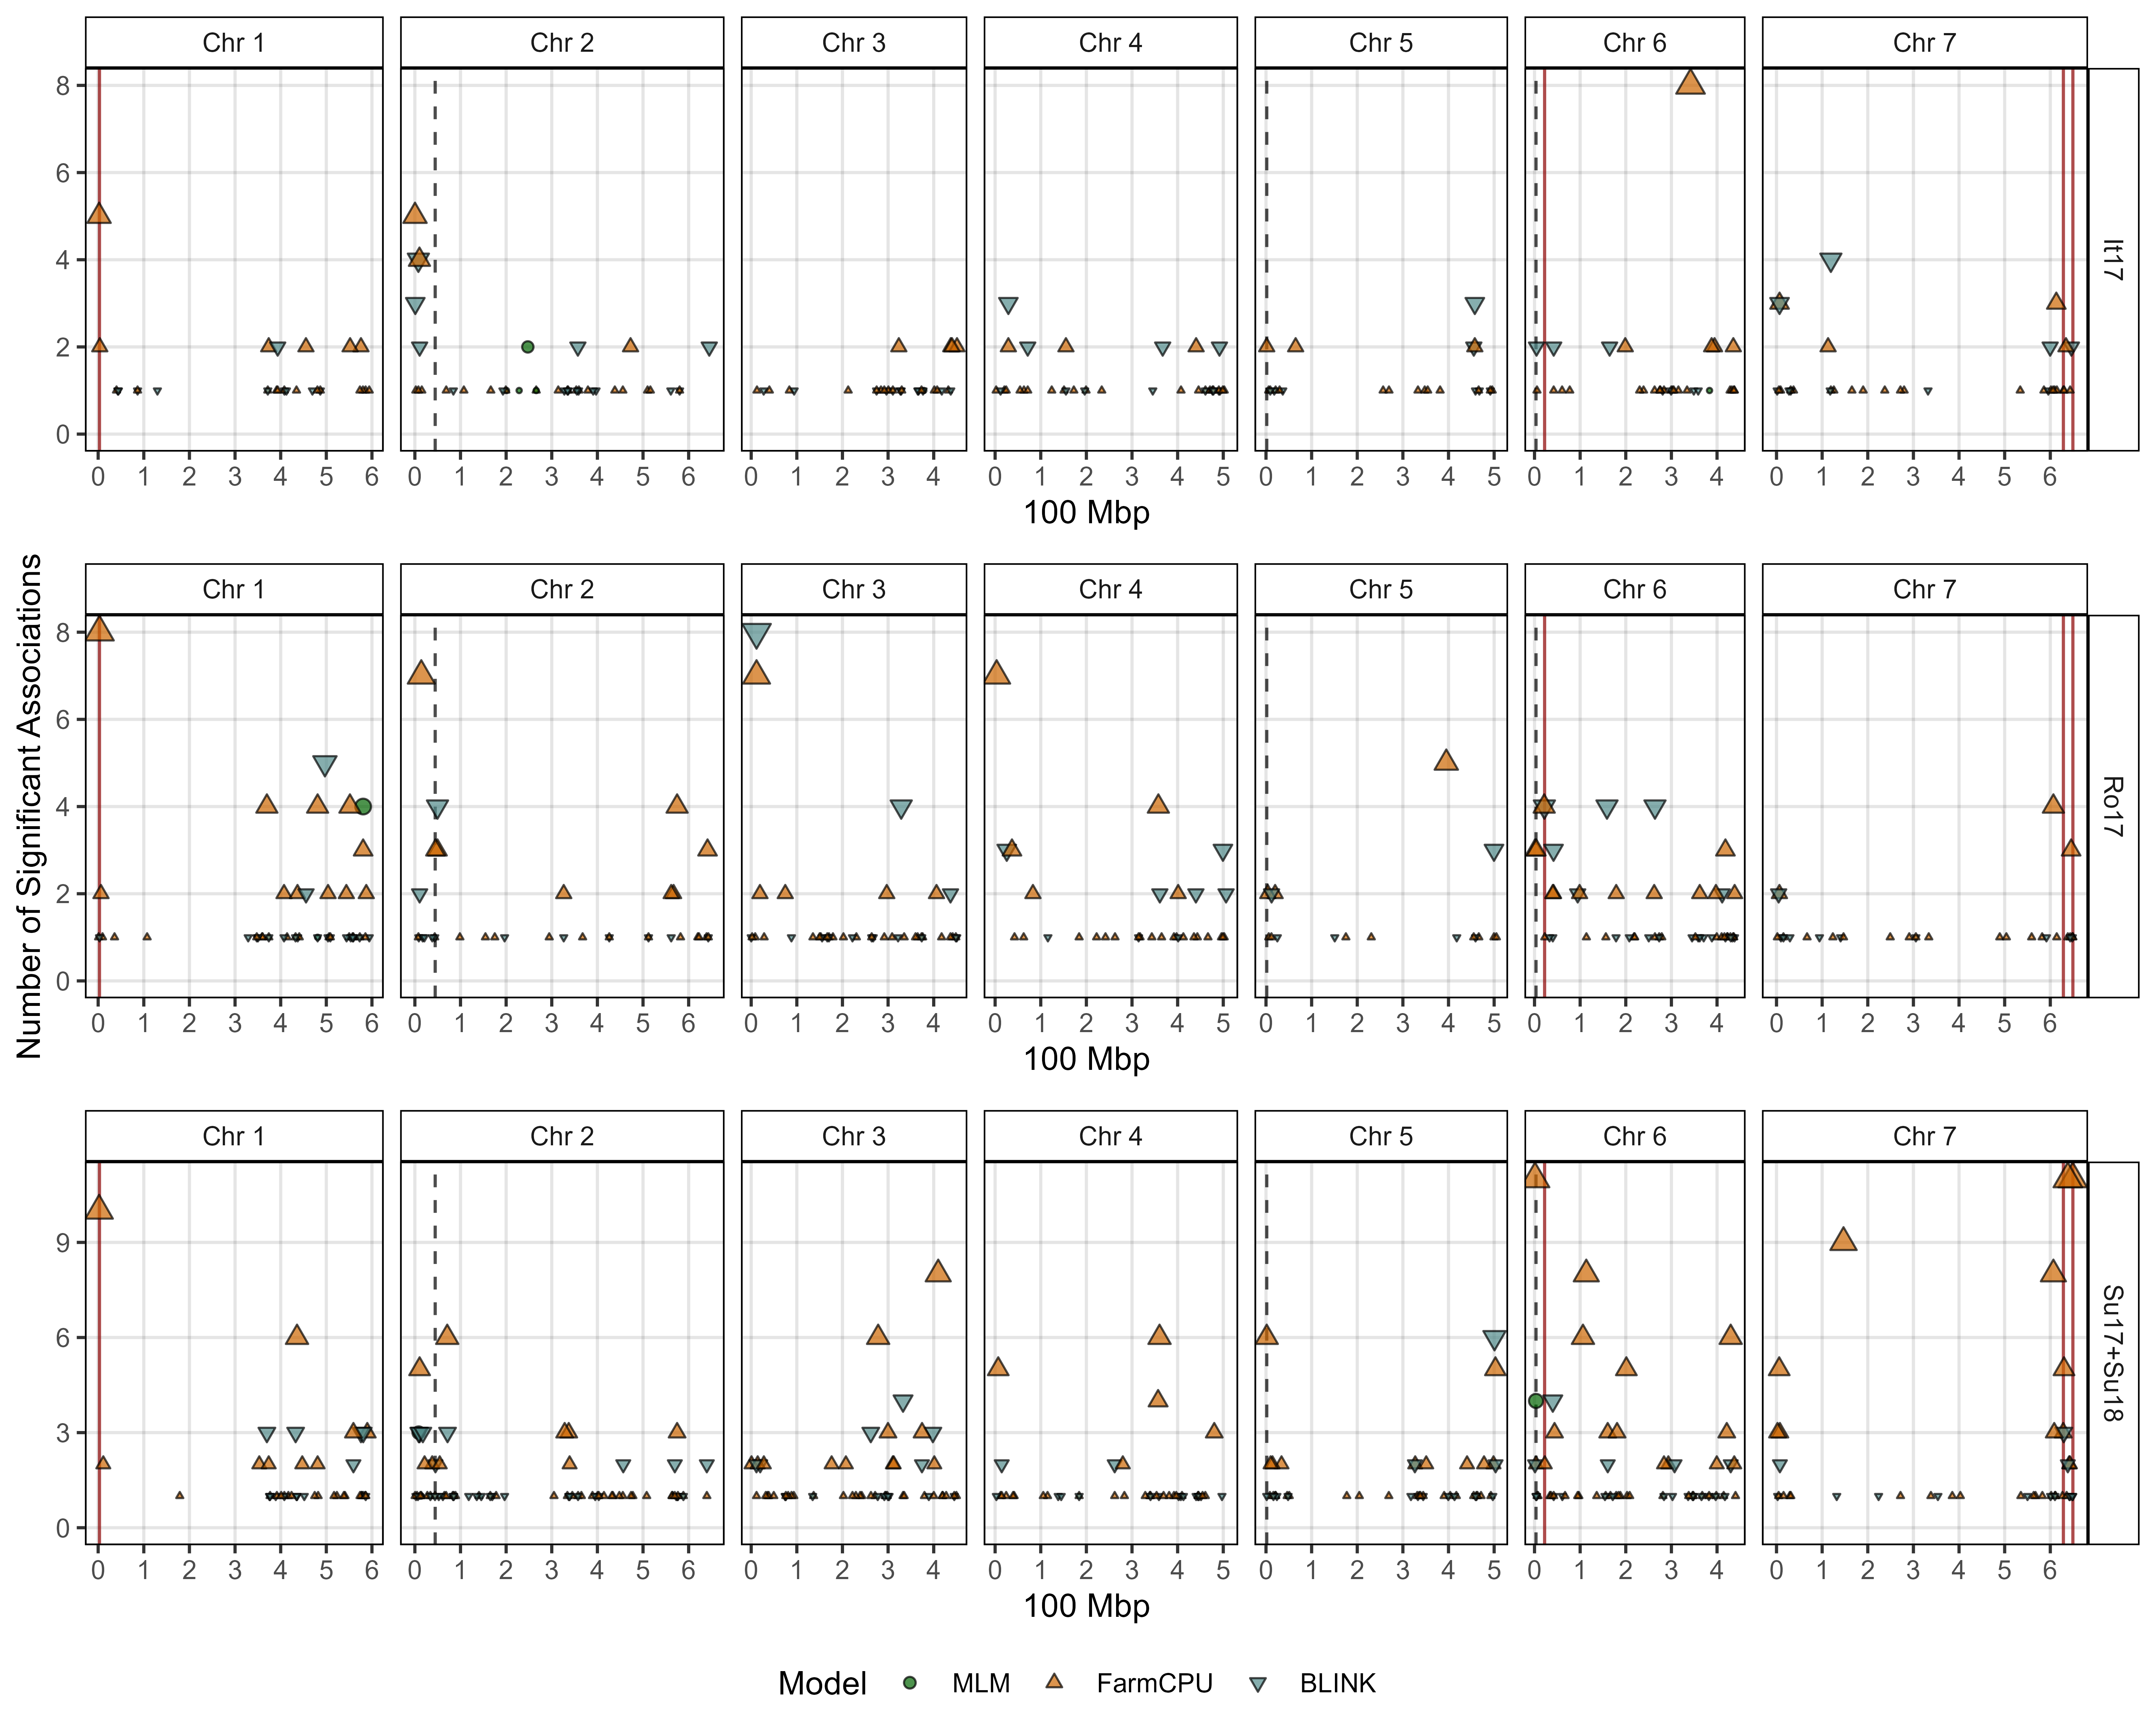
\includegraphics[keepaspectratio]{Supplemental_Figure_06.jpg}}

\begin{center}\rule{0.5\linewidth}{0.5pt}\end{center}

\subsection{Supplemental Figure 7}\label{supplemental-figure-7}

\pandocbounded{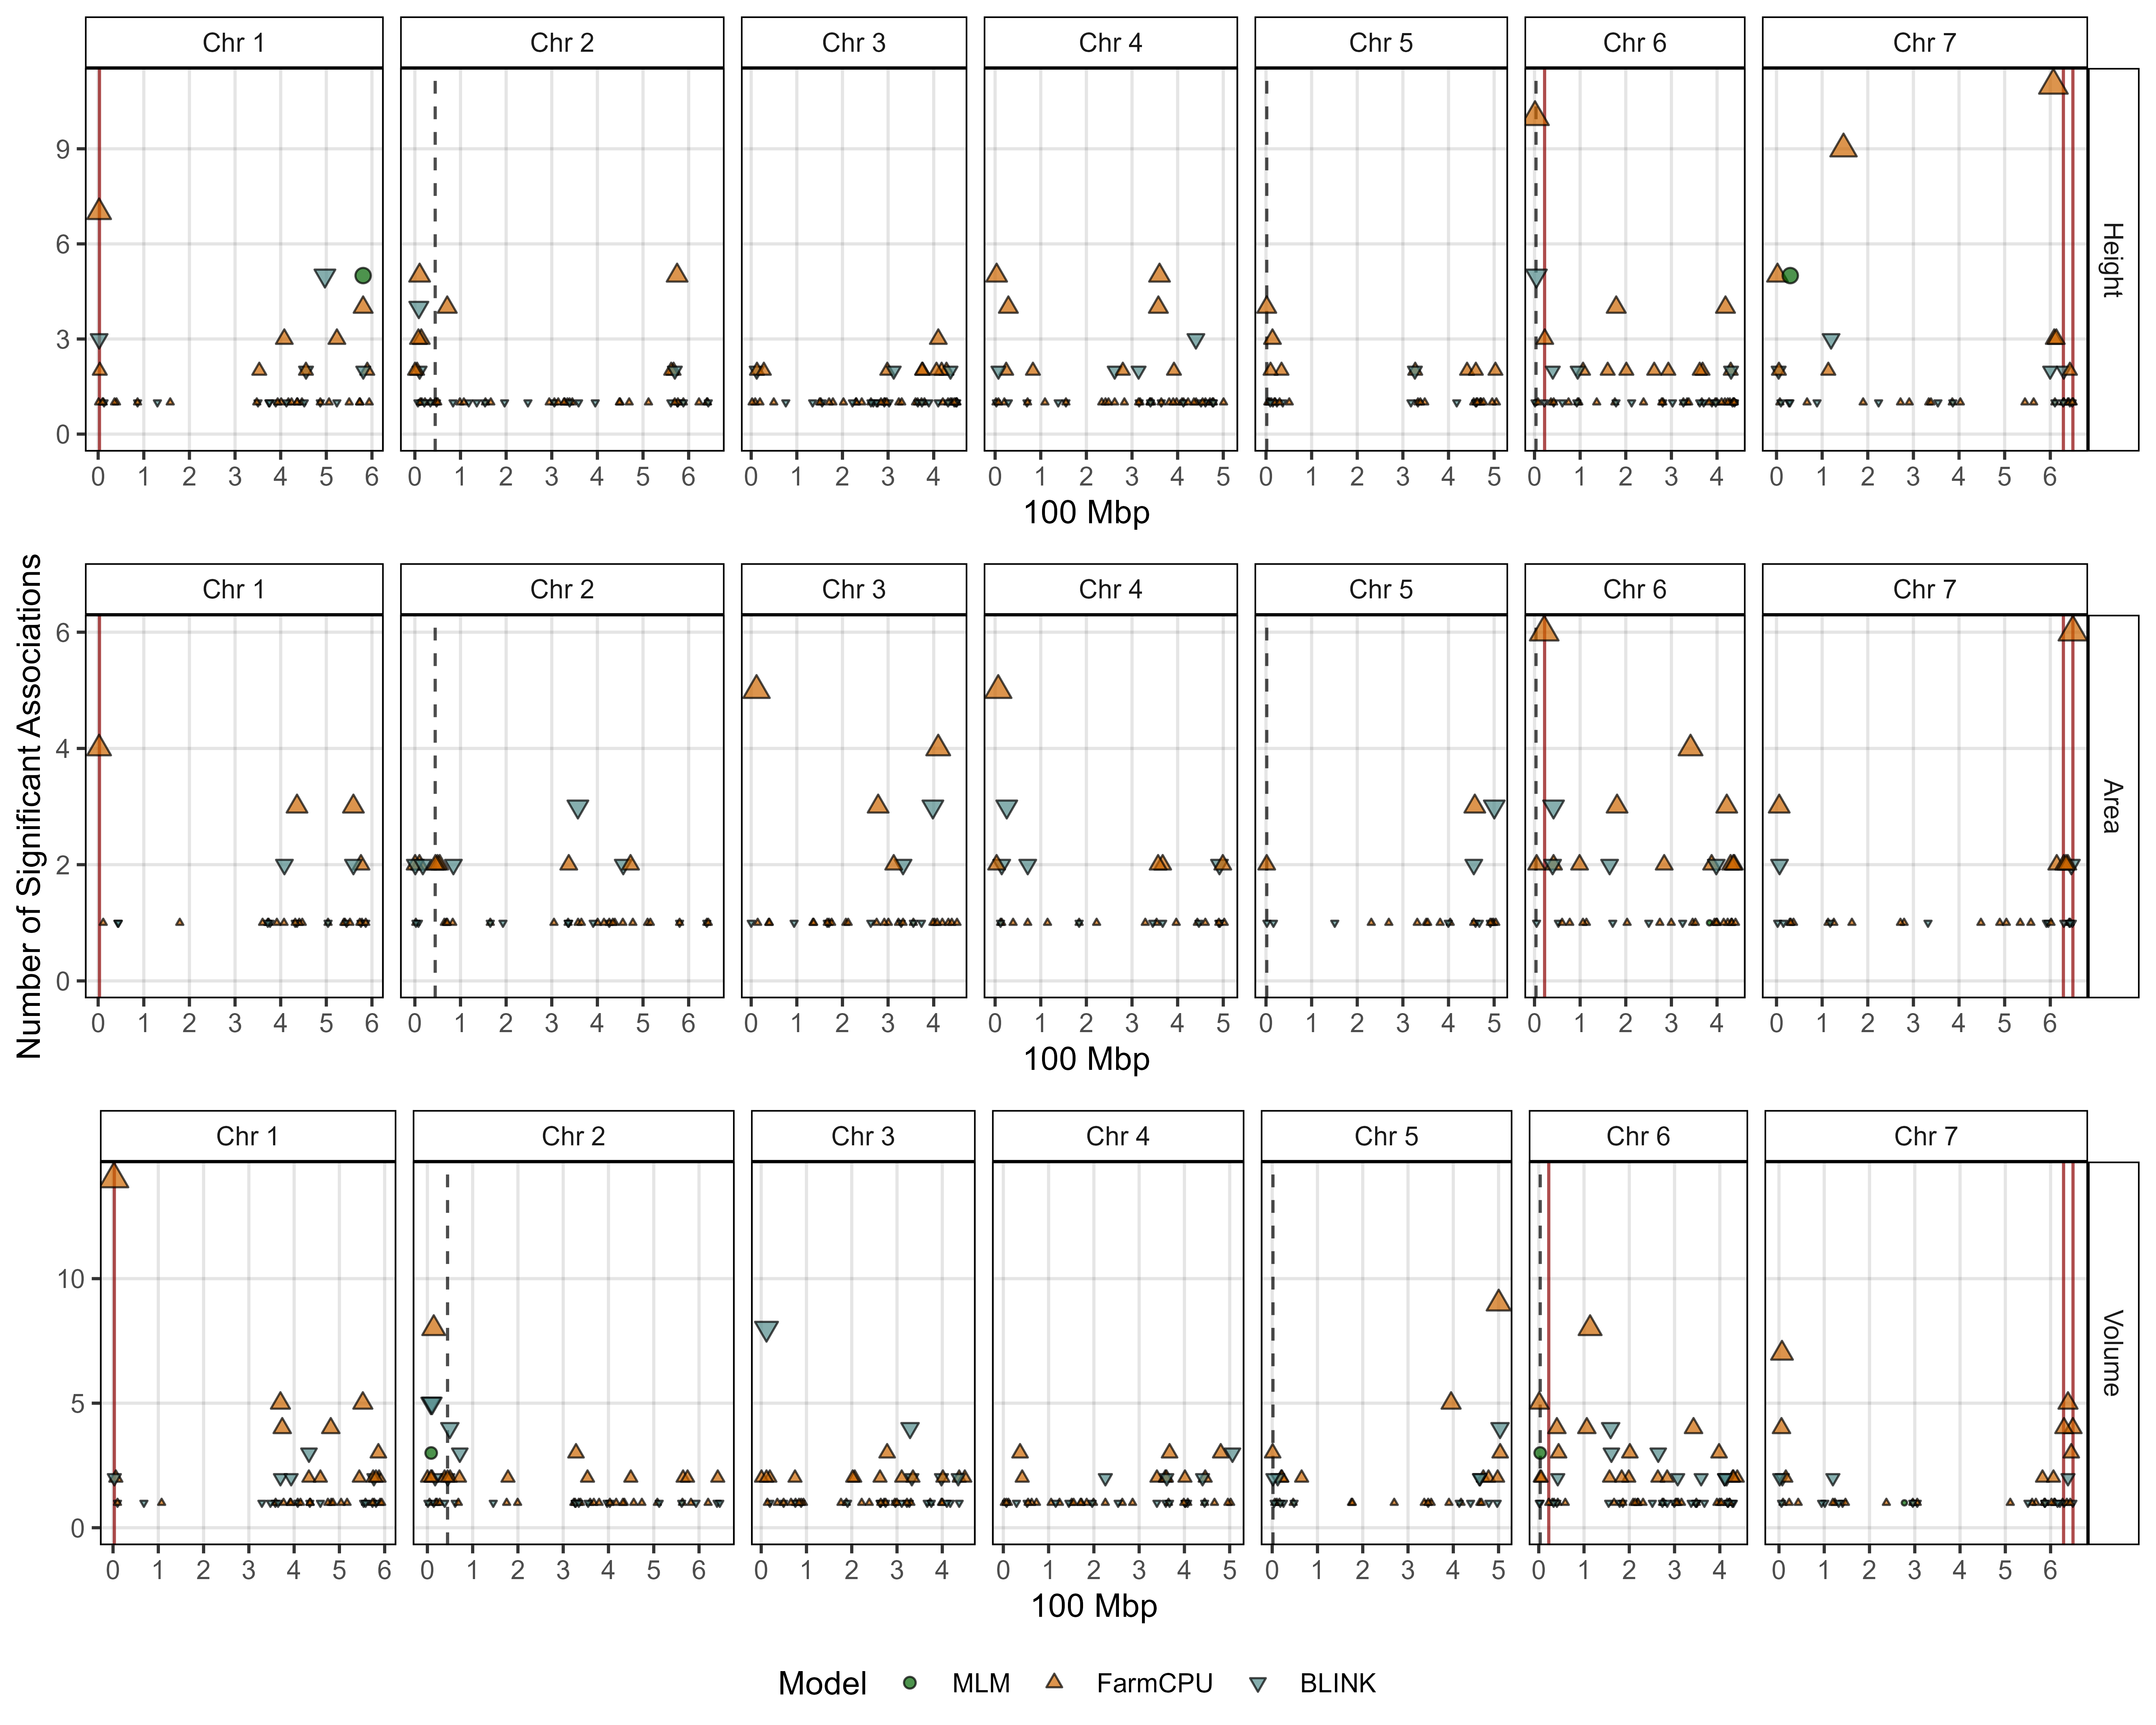
\includegraphics[keepaspectratio]{Supplemental_Figure_07.jpg}}

\begin{center}\rule{0.5\linewidth}{0.5pt}\end{center}

\subsection{Supplemental Figure 8}\label{supplemental-figure-8}

\pandocbounded{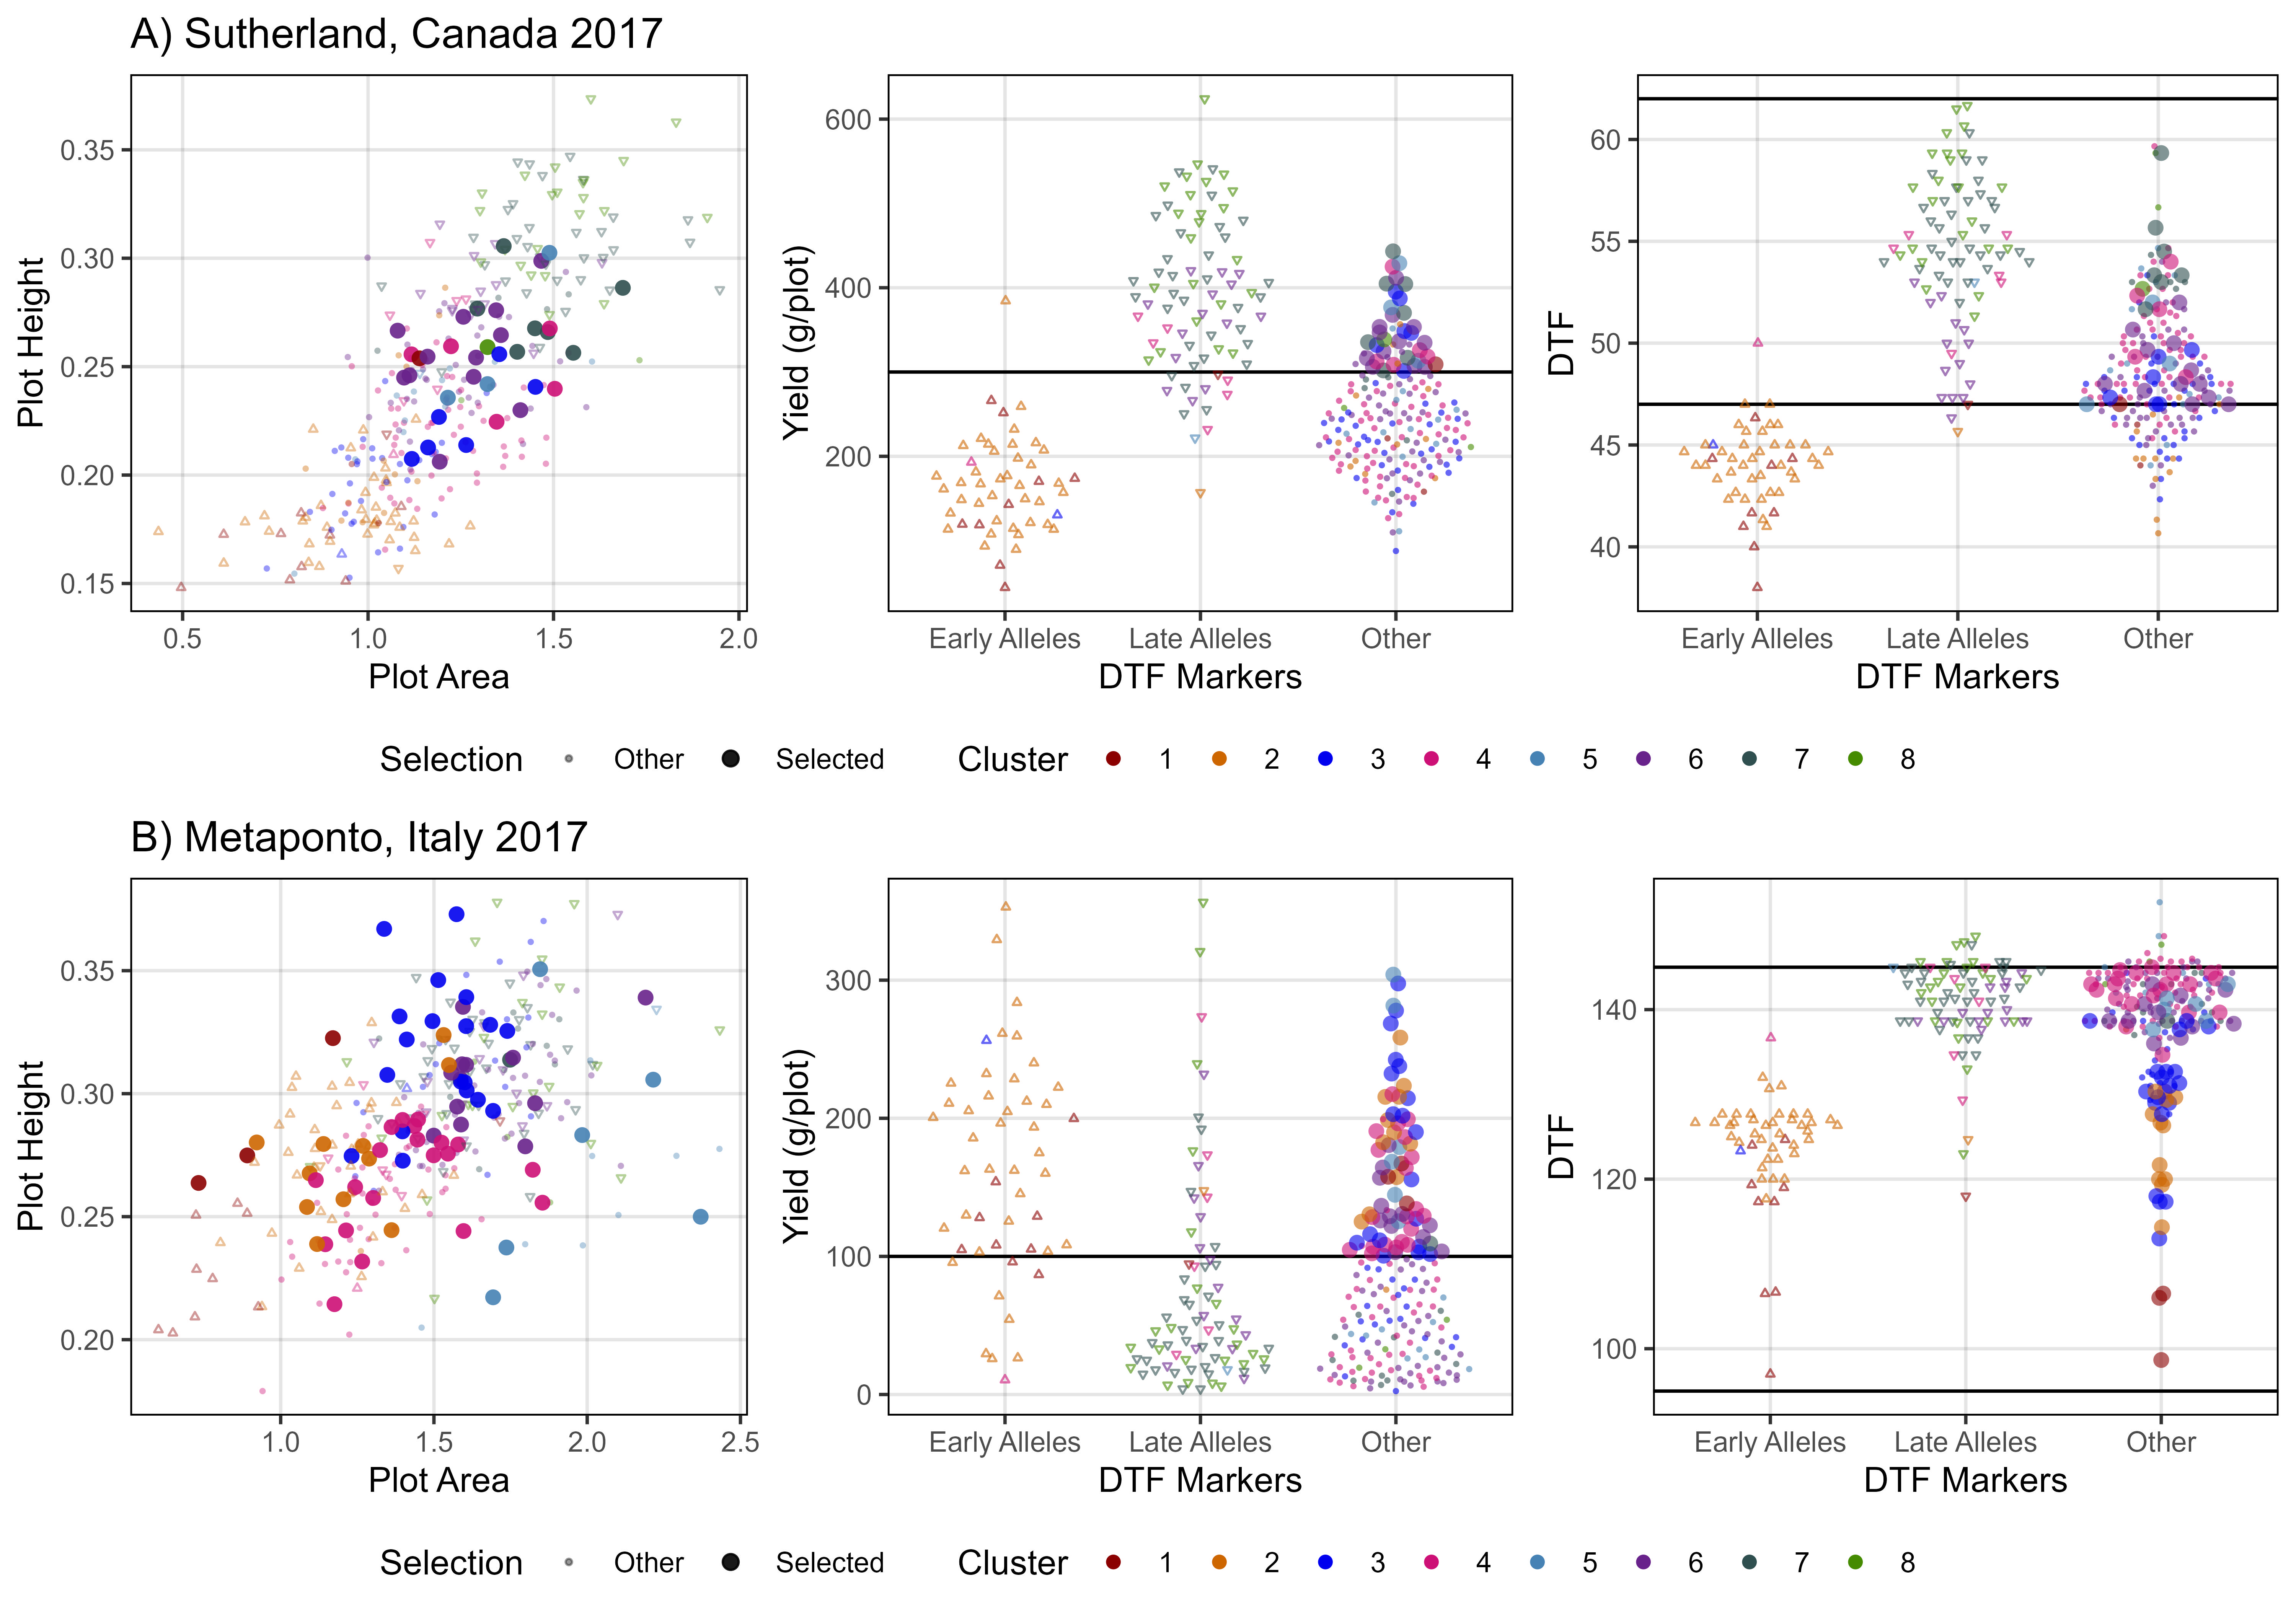
\includegraphics[keepaspectratio]{Supplemental_Figure_08.jpg}}

\begin{center}\rule{0.5\linewidth}{0.5pt}\end{center}

© Derek Michael Wright

\end{document}
